This section describes the background estimation methods used in the HH analysis. 

The simulated event samples summarised in Section~\ref{sec:data_backgrounds} are used to model all background processes, except for processes with fake-\tauhad which are estimated using data-driven techniques, as discussed below. In the \lephad channel, all fake-\tauhad backgrounds from $t\bar{t}$ and multi-jet processes are estimated using an inclusive fake-factor method, described in Section~\ref{subsec:LepHadfake}. In the \hadhad channel, the multijet background is estimated using a data-driven fake-factor method as described in Section~\ref{subsec:HadHadmultijet} and the $t\bar{t}$ background with fake-\tauhad is estimated using a scale-factor method with scale-factors derived from data to correct the MC prediction as described in Section~\ref{sec:ttbarfake_hadhad_sf_method}.

Separate estimation techniques are used for fake \tauhad from
multi-jet and \ttbar processes, since a combined approach is difficult
in the \hadhad-channel where multi-jet features two fake-\tauhad while
typically only a single fake-\tauhad is present in \ttbar. Moreover,
the presence of HLT \tauhad identification due to the \hadhad trigger
selection (cf.~\Cref{sec:hadhad_trigger_selection}) and the
requirement of at least one loose \tauhad in the derivation skim
introduces difficulties in combined estimation procedures. The larger
uncertainties, as compared to a combined approach, are not causing any
degradation of the results due the statistical limitation of the Run 2
analysis.

The \ttbar with true-\tauhad and Z+HF templates are taken from the MC prediction but their normalisations are derived from data as included as freely floating parameters in the final fit, as described in Section~\ref{sec:fit}. 

Events with electrons or muons that are misidentified as \tauhad\ objects, dominantly coming from the \ttbar\ production, represent a minor background in the analysis and they are estimated from simulation. This background is treated together with the \ttbar\ events containing true-\tauhad\ objects. Additional material can be found in Appendix~\ref{subsec:appendix_bkg_leptons_faking_taus}.


\subsection{Fake-$\tau$ backgrounds in the \lephad channel}
\label{subsec:LepHadfake}

In the \lephad channel, the strategy for modeling background processes where the hadronic tau is faked by a jet follows 
closely the technique described in section 5.3 of reference \cite{AlvarezPiqueras:2131232} to derive a \tauhad `fake-factor' 
in order to weight fake-\tauhad events. Fake-factors are calculated separately for SLT and LTT categories. 

The dominant source of fake-\tauhad candidates in the 2 $b$-tag signal region comes from \ttbar events, with smaller contributions from multi-jet process. 
No attempt is made to account for the negligible \Wjets process  when deriving fake-factors.
%In the 0 $b$-tag region the fake-\tauhad background is dominated by \Wjets events, while the 1 $b$-tag region has a roughly equal split of \ttbar and \Wjets events dominating the fake-\tauhad contribution. 
%Fake-factors are not derived separately for the electron and muon channels, since the probability for a jet to fake a \tauhad is 
%independent of the flavor of any accompanying charged lepton in the event. This assumption is checked and 
%no significant difference is found between the fake-factors calculated for the electron channel and those for the muon channel. 

Fake-factors ($FF$) are calculated separately for \ttbar and multi-jet, and for 1 and 3-prong \tauhad candidates. 
They are parameterised in terms of \pT(\tauhad) requiring opposite-sign lepton-tau pairs, as shown in Figures \ref{fig:SLT_FF} and \ref{fig:LTT_FF}, for the SLT and LTT categories, respectively.
For each process the $FF$ are calculated in a dedicated background enriched region. The control regions for each process are defined as follows:
 \begin{itemize}
 	\item Multi-jet: inverted lepton isolation (`tight' electrons and `medium' muons are required to fail their respective ‘loose’ isolation working points), 2 b-tag. 
 	\item \ttbar: \mbb > 150 GeV, 2 $b$-tag 
 \end{itemize}
 
A fake-\tauhad enriched sample is defined by applying the full selection defined in the signal region and in each control region, 
but requiring that the loose \tauhad is replaced by an anti-\tauhad object (failing the loose $\tau$-ID requirement, but with a RNN score > 0.01). 
In the case where the event contains more than one anti-\tauhad, one is chosen randomly. Derived variables used in the analysis,
such as the \MET, $m^{\mathrm{MMC}}_\mathrm{T}$ and \MET$\phi$ centrality are calculated in the same way as for signal events, 
but with the anti-\tauhad taking the place of the loose \tauhad candidate.

To demonstrate the purity of the desired backgrounds in the \ttbar and multi-jet control regions, 
we have included distributions of the $\tau$ $p_T$ for the control regions with the \tauhad and 
anti-\tauhad requirements, separately for 1-prong and 3-prong \tauhad.  These distributions can 
be seen in Fig.~\ref{fig:ttbarCR_1}, Fig.~\ref{fig:ttbarCR_3}, Fig.~\ref{fig:QCD_CR_1},  and Fig.~\ref{fig:QCD_CR_3}, 
where the fake contribution is taken from Monte Carlo only.  Thus, the gap between the Monte Carlo prediction and data in the multi-jet CR is attributed to multi-jet events, which are not simulated for this analysis. For simulated backgrounds, the yields can be seen in the legend.

\begin{figure}
\centering
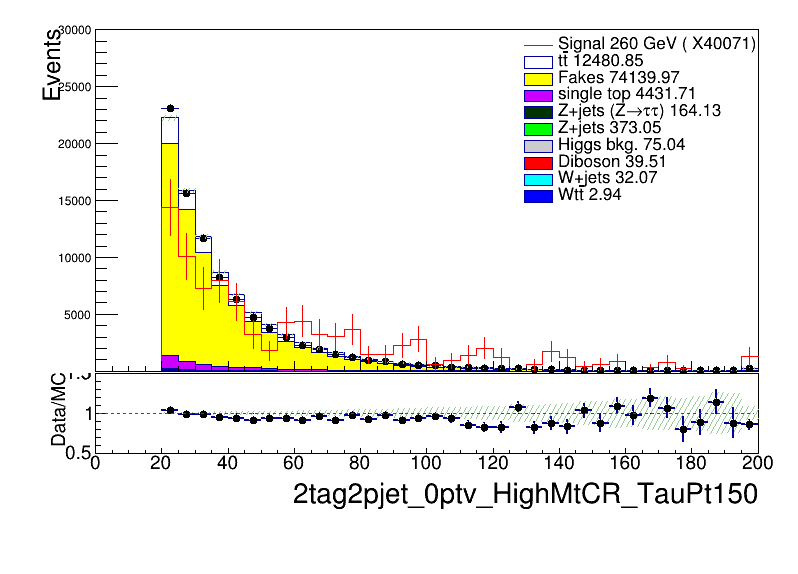
\includegraphics[width=.45\textwidth]{figures/lephadFF/SLT/2tag2pjet_0ptv_HighMtCR_TauPt150_CR_SLT_ALL_ttWeight_1.png}
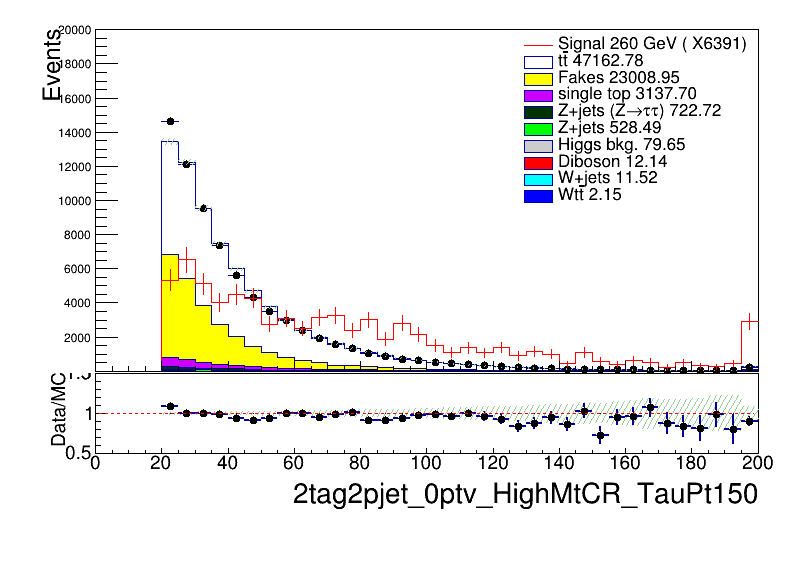
\includegraphics[width=.45\textwidth]{figures/lephadFF/SLT/2tag2pjet_0ptv_HighMtCR_TauPt150_SR_SLT_ALL_ttWeight_1.png} \\
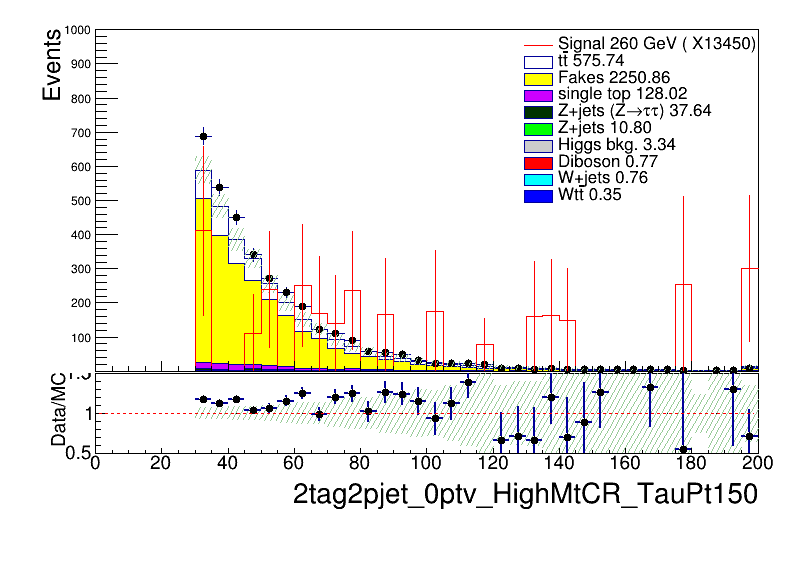
\includegraphics[width=.45\textwidth]{figures/lephadFF/LTT/2tag2pjet_0ptv_HighMtCR_TauPt150_CR_LTT_ALL_ttWeight_1.png}
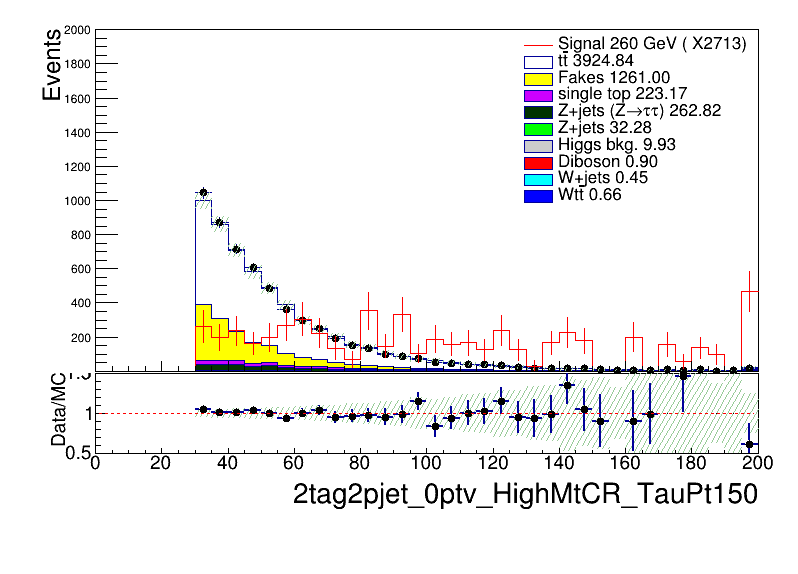
\includegraphics[width=.45\textwidth]{figures/lephadFF/LTT/2tag2pjet_0ptv_HighMtCR_TauPt150_SR_LTT_ALL_ttWeight_1.png}\\
\caption{Plots of the $\tauhad$ $p_T$ distributions for the (left) anti-\tauhad and (right) \tauhad selection for the (top) single lepton trigger and (bottom) lepton-plus-tau trigger selections in the \ttbar control region with 1-prong \tauhad.}
\label{fig:ttbarCR_1}
\end{figure} 

\begin{figure}
\centering
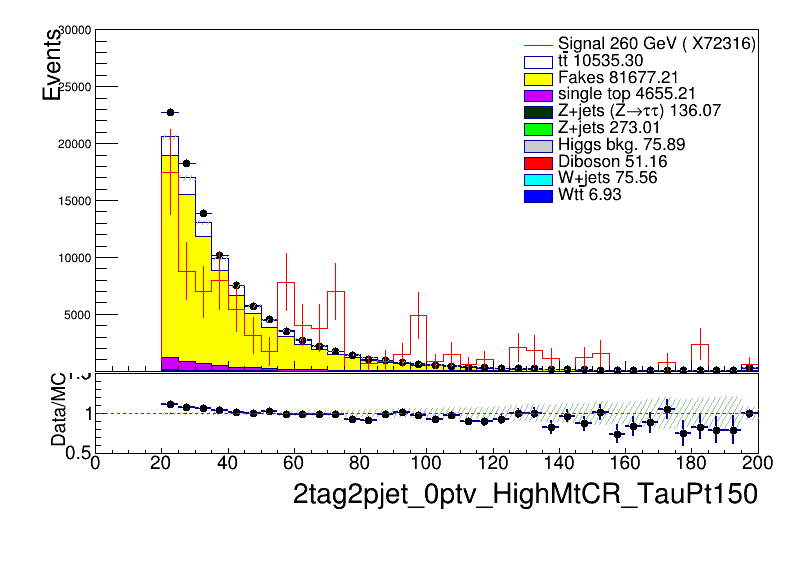
\includegraphics[width=.45\textwidth]{figures/lephadFF/SLT/2tag2pjet_0ptv_HighMtCR_TauPt150_CR_SLT_ALL_ttWeight_3.png}
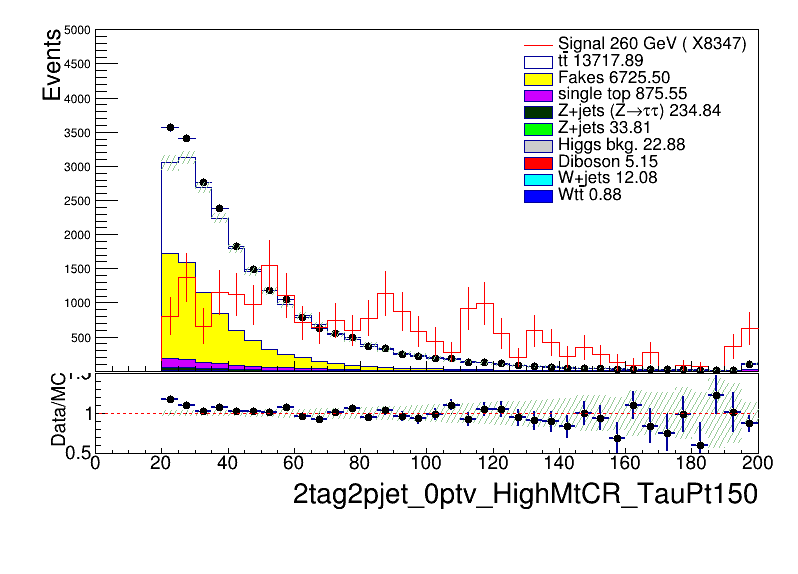
\includegraphics[width=.45\textwidth]{figures/lephadFF/SLT/2tag2pjet_0ptv_HighMtCR_TauPt150_SR_SLT_ALL_ttWeight_3.png} \\
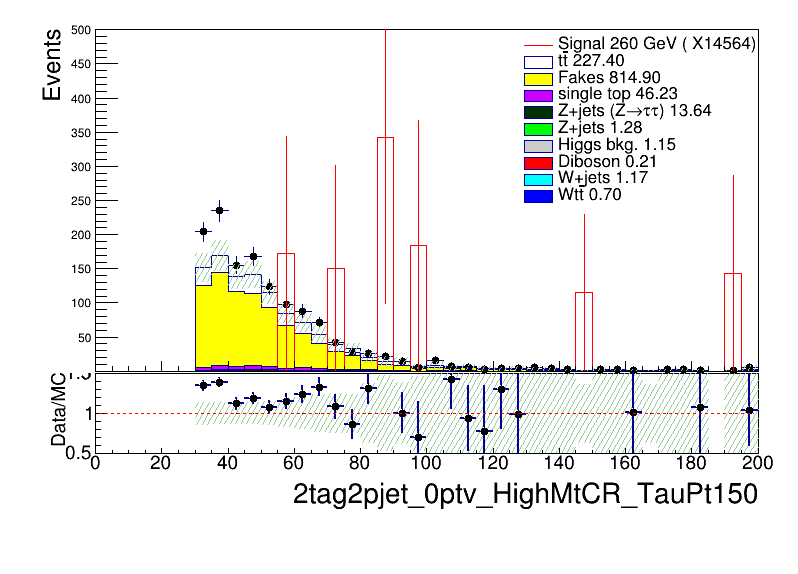
\includegraphics[width=.45\textwidth]{figures/lephadFF/LTT/2tag2pjet_0ptv_HighMtCR_TauPt150_CR_LTT_ALL_ttWeight_3.png}
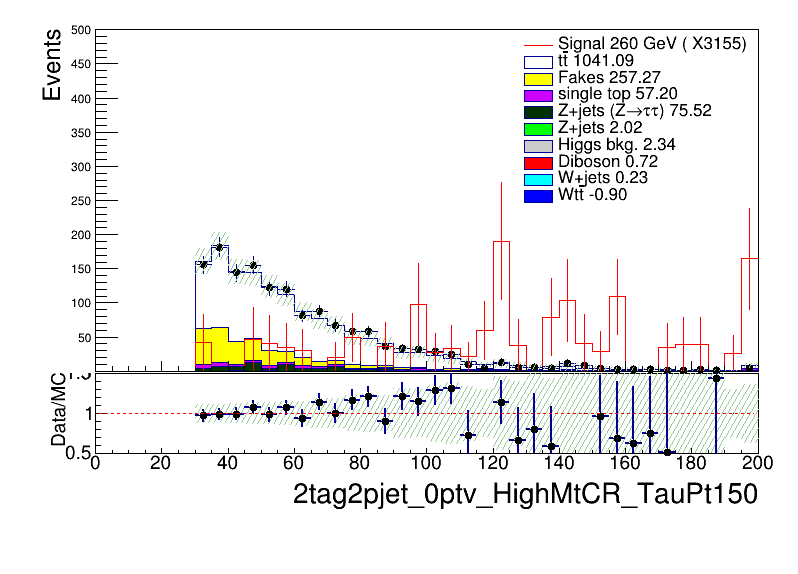
\includegraphics[width=.45\textwidth]{figures/lephadFF/LTT/2tag2pjet_0ptv_HighMtCR_TauPt150_SR_LTT_ALL_ttWeight_3.png}\\
\caption{Plots of the $\tauhad$ $p_T$ distributions for the (left) anti-\tauhad and (right) \tauhad selection for the (top) single lepton trigger and (bottom) lepton-plus-tau trigger selections in the \ttbar control region with 3-prong \tauhad.}
\label{fig:ttbarCR_3}
\end{figure}

\begin{figure}
\centering
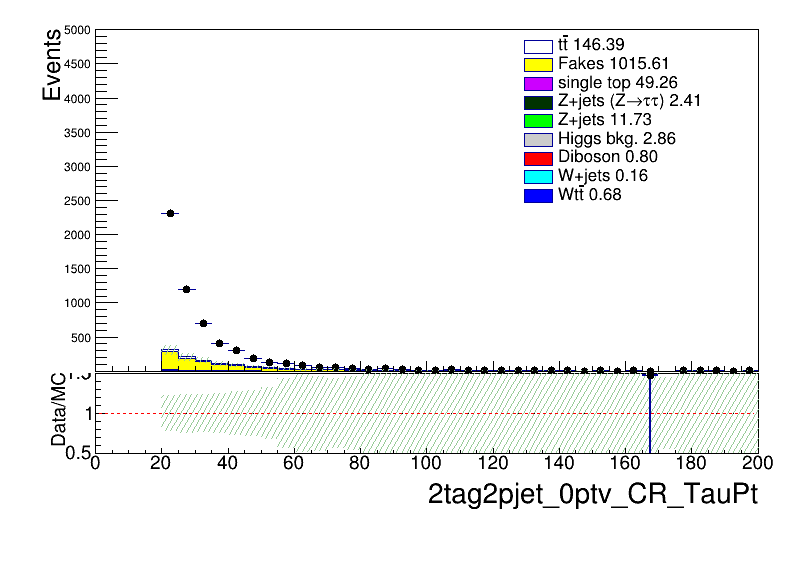
\includegraphics[width=.45\textwidth]{figures/lephadFF/SLT/2tag2pjet_0ptv_CR_TauPt_IICR_SLT_ALL_ttWeight_1.png}
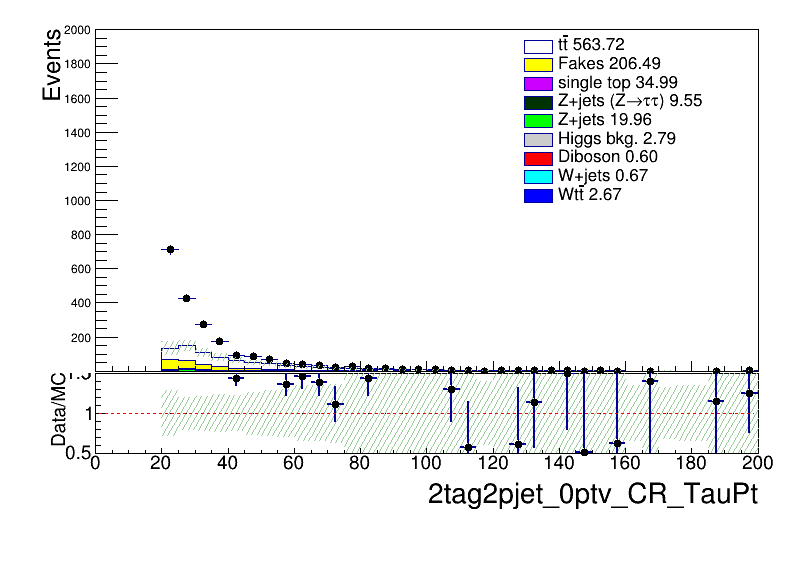
\includegraphics[width=.45\textwidth]{figures/lephadFF/SLT/2tag2pjet_0ptv_CR_TauPt_IISR_SLT_ALL_ttWeight_1.png} \\
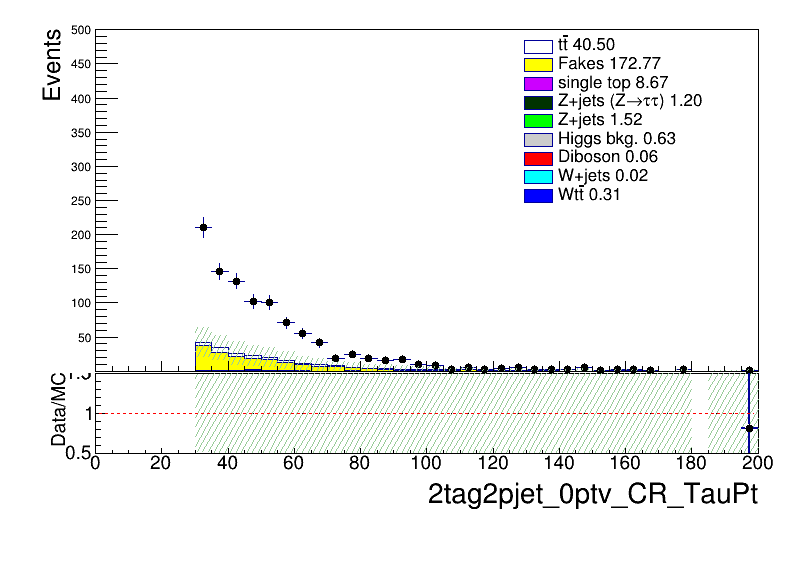
\includegraphics[width=.45\textwidth]{figures/lephadFF/LTT/2tag2pjet_0ptv_CR_TauPt_IICR_LTT_ALL_ttWeight_1.png}
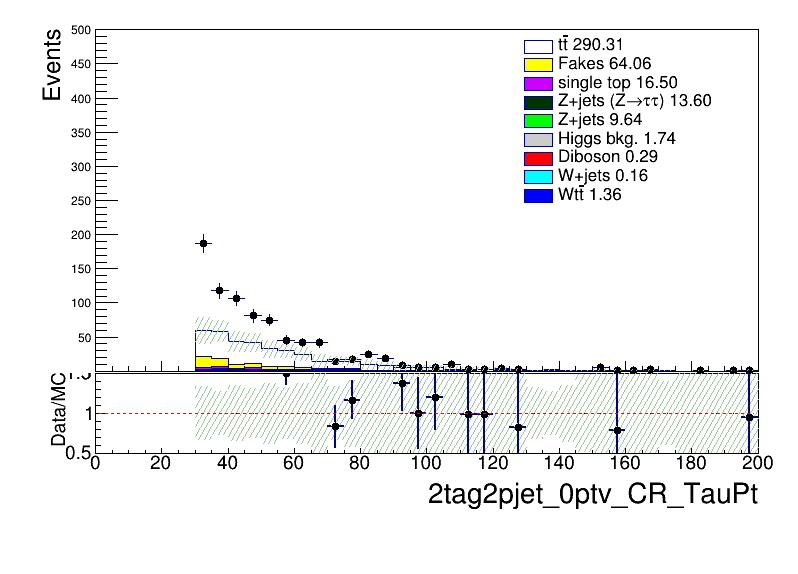
\includegraphics[width=.45\textwidth]{figures/lephadFF/LTT/2tag2pjet_0ptv_CR_TauPt_IISR_LTT_ALL_ttWeight_1.png}\\
\caption{Plots of the $\tauhad$ $p_T$ distributions for the (left) anti-\tauhad and (right) \tauhad selection for the (top) single lepton trigger and (bottom) lepton-plus-tau trigger selections in the multi-jet control region with 1-prong \tauhad.}
\label{fig:QCD_CR_1}
\end{figure}

\begin{figure}
\centering
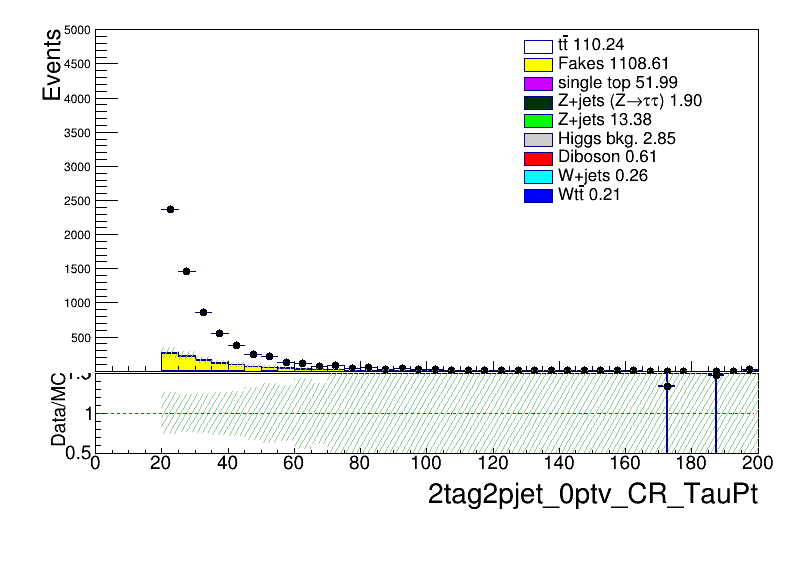
\includegraphics[width=.45\textwidth]{figures/lephadFF/SLT/2tag2pjet_0ptv_CR_TauPt_IICR_SLT_ALL_ttWeight_3.png}
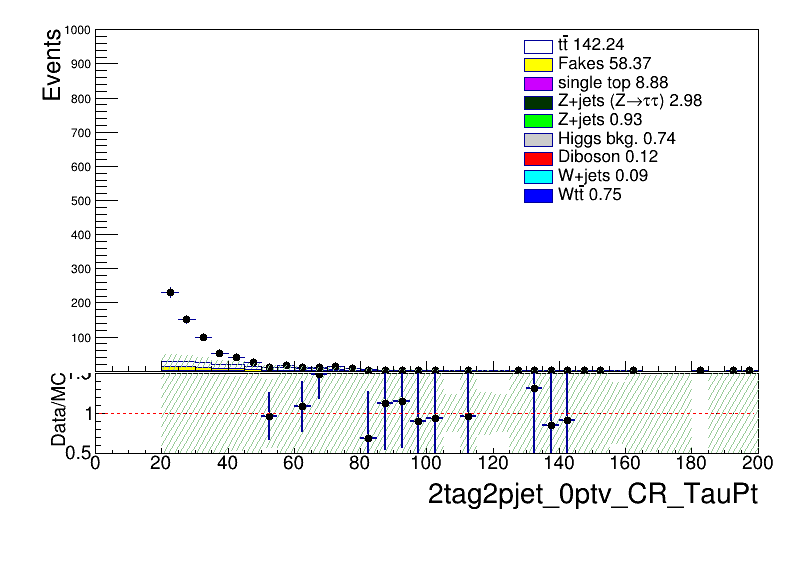
\includegraphics[width=.45\textwidth]{figures/lephadFF/SLT/2tag2pjet_0ptv_CR_TauPt_IISR_SLT_ALL_ttWeight_3.png} \\
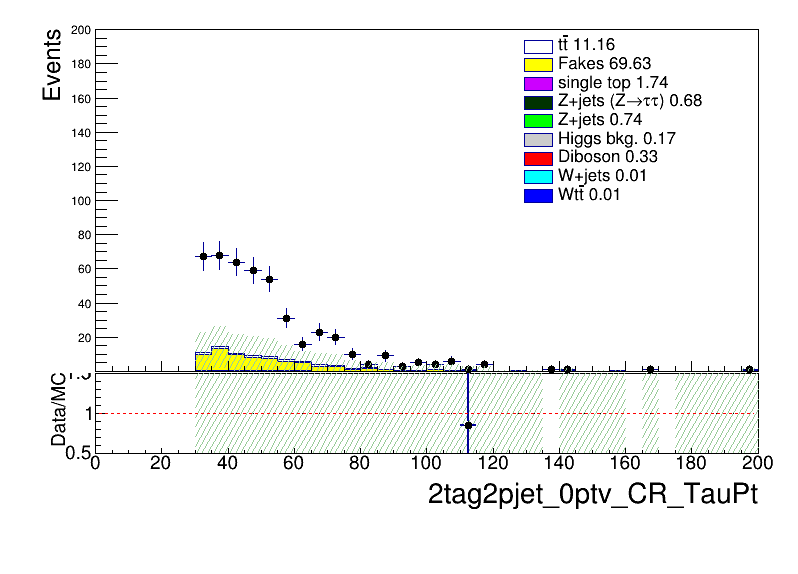
\includegraphics[width=.45\textwidth]{figures/lephadFF/LTT/2tag2pjet_0ptv_CR_TauPt_IICR_LTT_ALL_ttWeight_3.png}
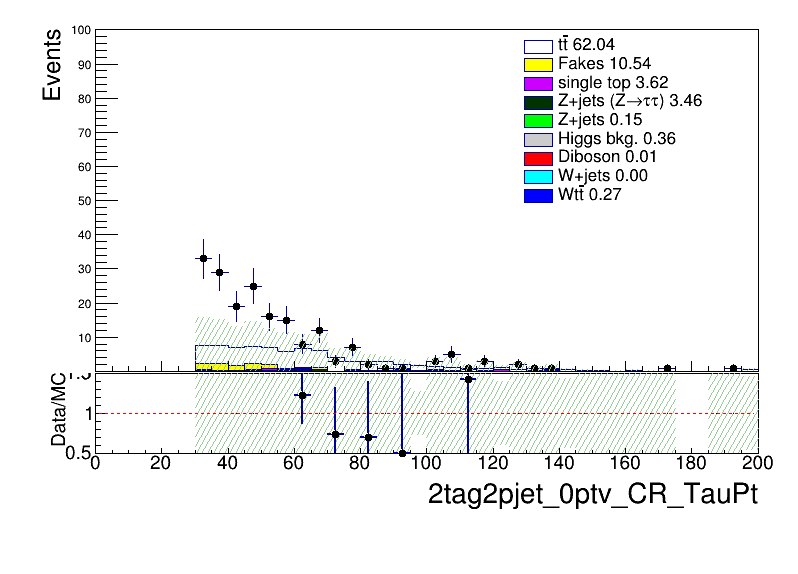
\includegraphics[width=.45\textwidth]{figures/lephadFF/LTT/2tag2pjet_0ptv_CR_TauPt_IISR_LTT_ALL_ttWeight_3.png}\\
\caption{Plots of the $\tauhad$ $p_T$ distributions for the (left) anti-\tauhad and (right) \tauhad selection for the (top) single lepton trigger and (bottom) lepton-plus-tau trigger selections in the multi-jet control region with 3-prong \tauhad.}
\label{fig:QCD_CR_3}
\end{figure}



The fake-factors are calculated as:

\begin{equation}
FF =  \frac{N(\text{loose }\tauhad)}{N(\mathrm{anti}\mhyphen\tauhad)}
\end{equation} 

where contributions from true hadronic taus and minor background processes are subtracted from 
each of the terms. Though the fake factors are parameterized only in $\tau$ $p_T$, they are also shown 
in Fig.~\ref{fig:lhFF_eta_SLT} and Fig.~\ref{fig:lhFF_eta_LTT} as a function of $\eta$, split only into barrel and endcap regions, to explore whether there is 
a significant dependence on $\tau$ $\eta$. There is no clear trend, which is why the fake factors are not parameterized in 
terms of $\eta$.

\begin{figure}
\centering
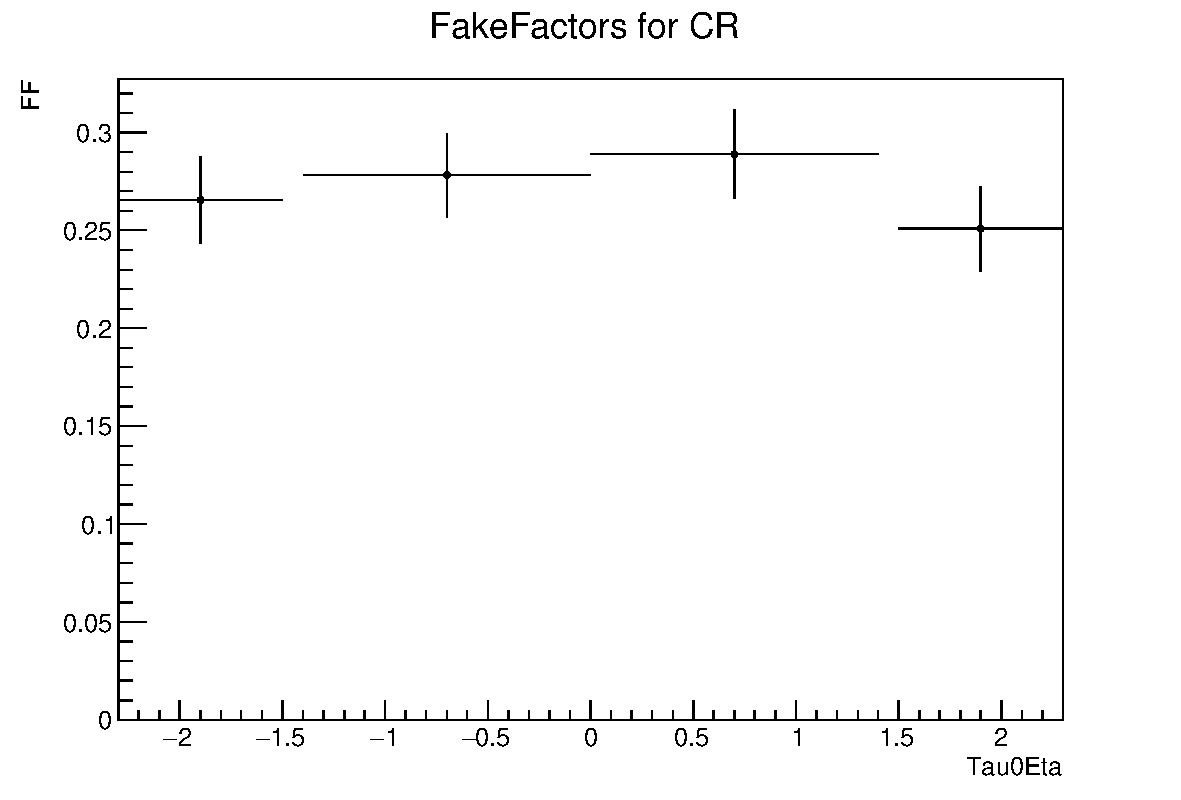
\includegraphics[width=.4\textwidth]{figures/lephadFF/SLT/FF_All_Preselection_Np1_CR_2tag_Tau0Eta}
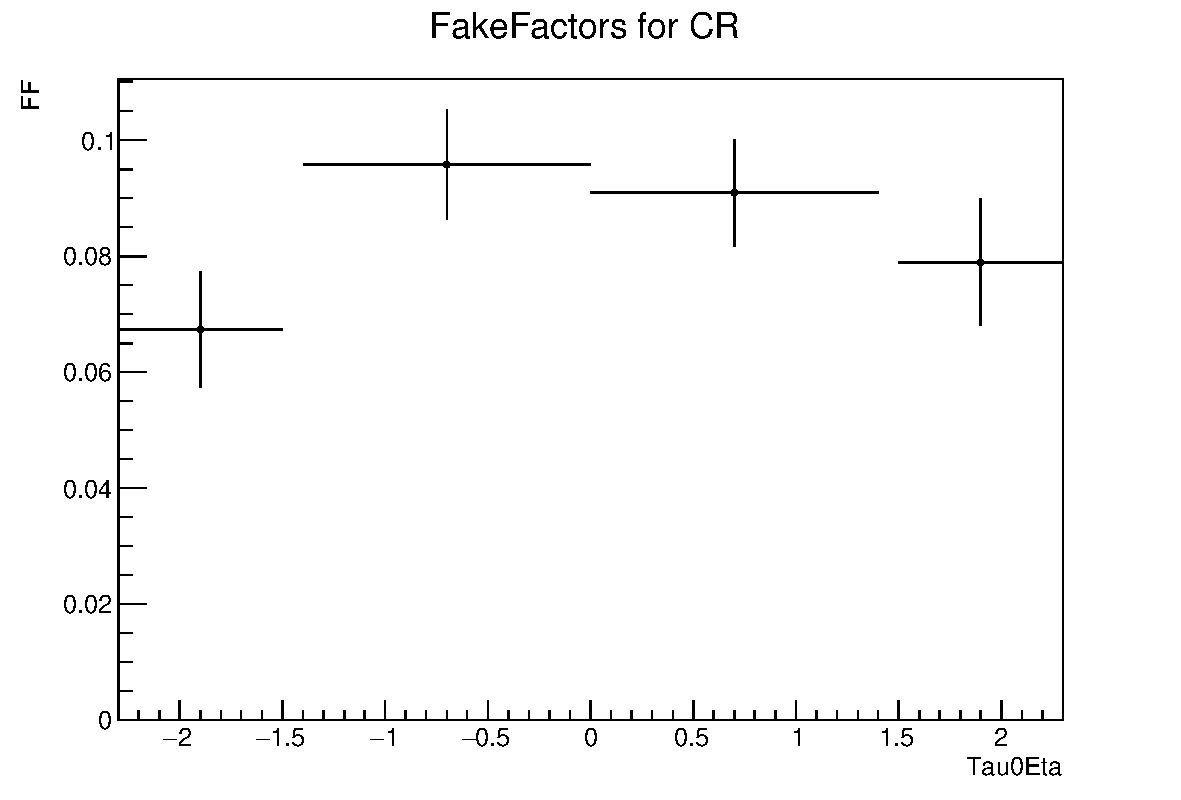
\includegraphics[width=.4\textwidth]{figures/lephadFF/SLT/FF_All_Preselection_Np3_CR_2tag_Tau0Eta} \\
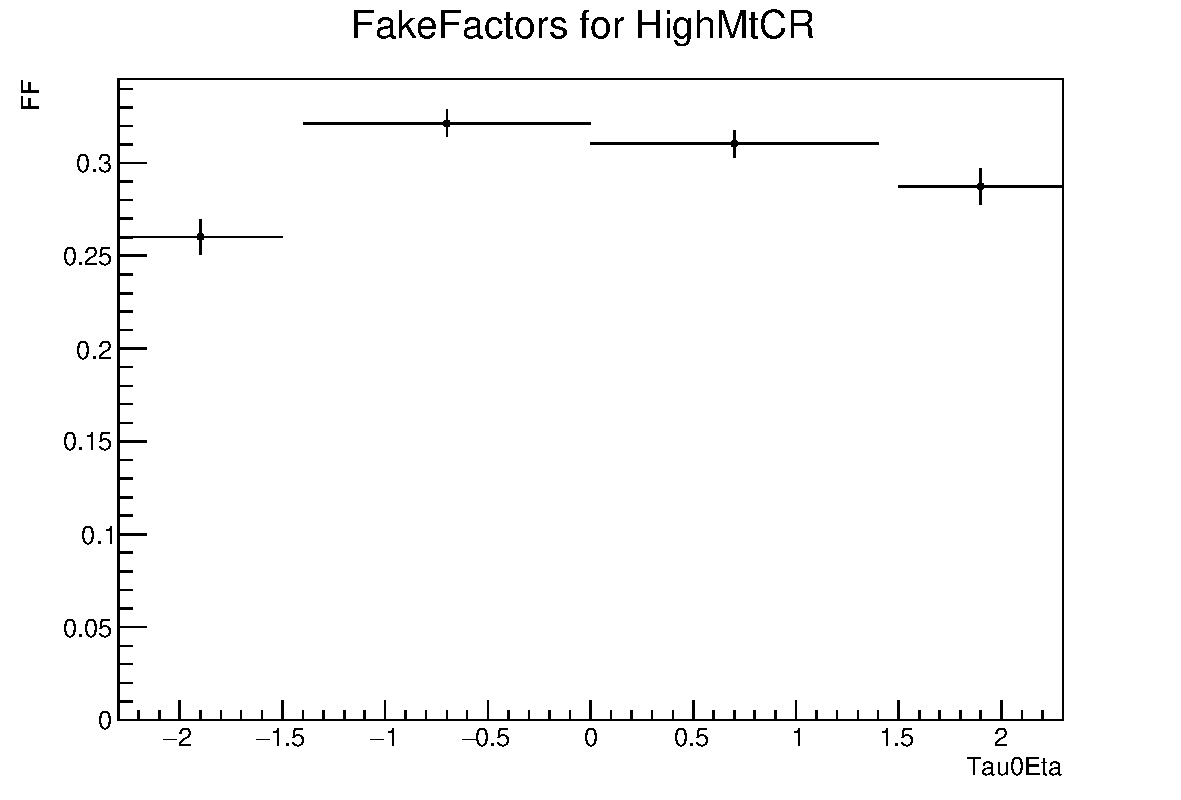
\includegraphics[width=.4\textwidth]{figures/lephadFF/SLT/FF_All_Preselection_Np1_HighMtCR_2tag_Tau0Eta}
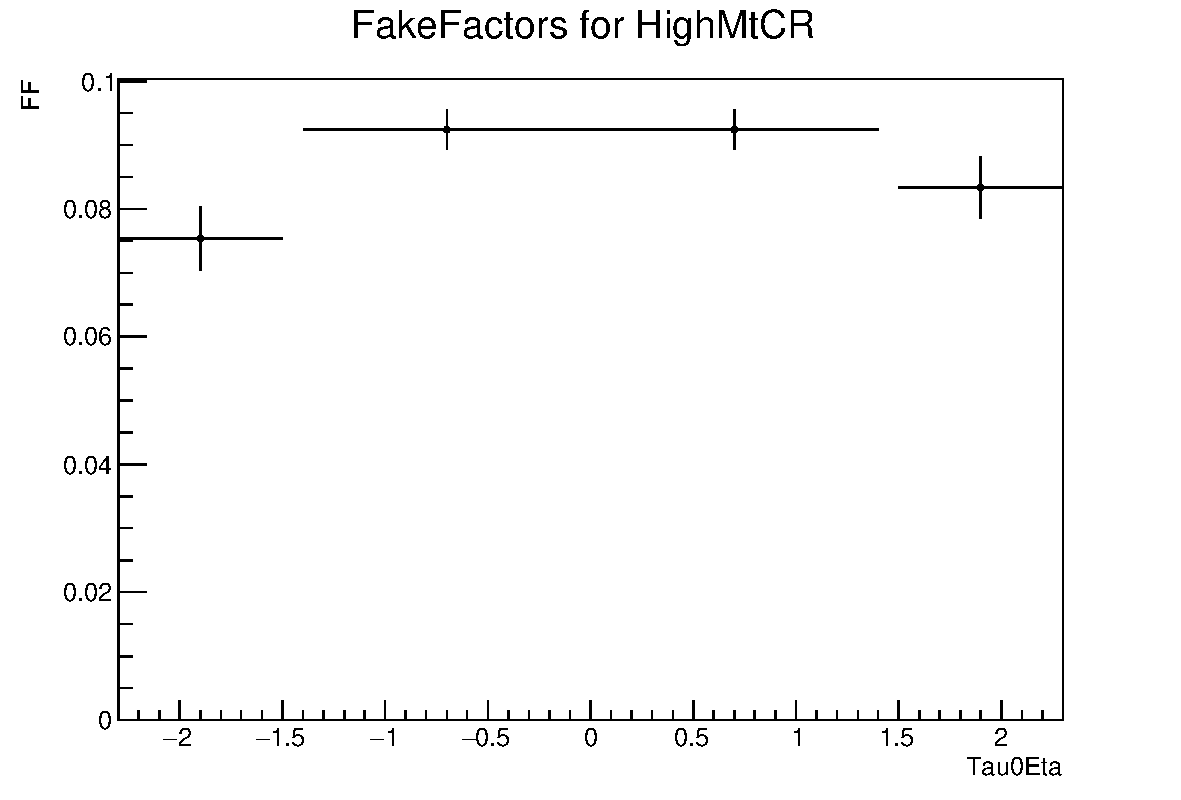
\includegraphics[width=.4\textwidth]{figures/lephadFF/SLT/FF_All_Preselection_Np3_HighMtCR_2tag_Tau0Eta}\\
\caption{Fake-factors as a function of $\eta$ for 1-prong (left) and 3-prong (right) \tauhad candidates for multi-jet (top) and \ttbar processes (bottom) for the \lephad SLT category. No significant trend is observed.}
\label{fig:lhFF_eta_SLT}
\end{figure}

\begin{figure}
\centering
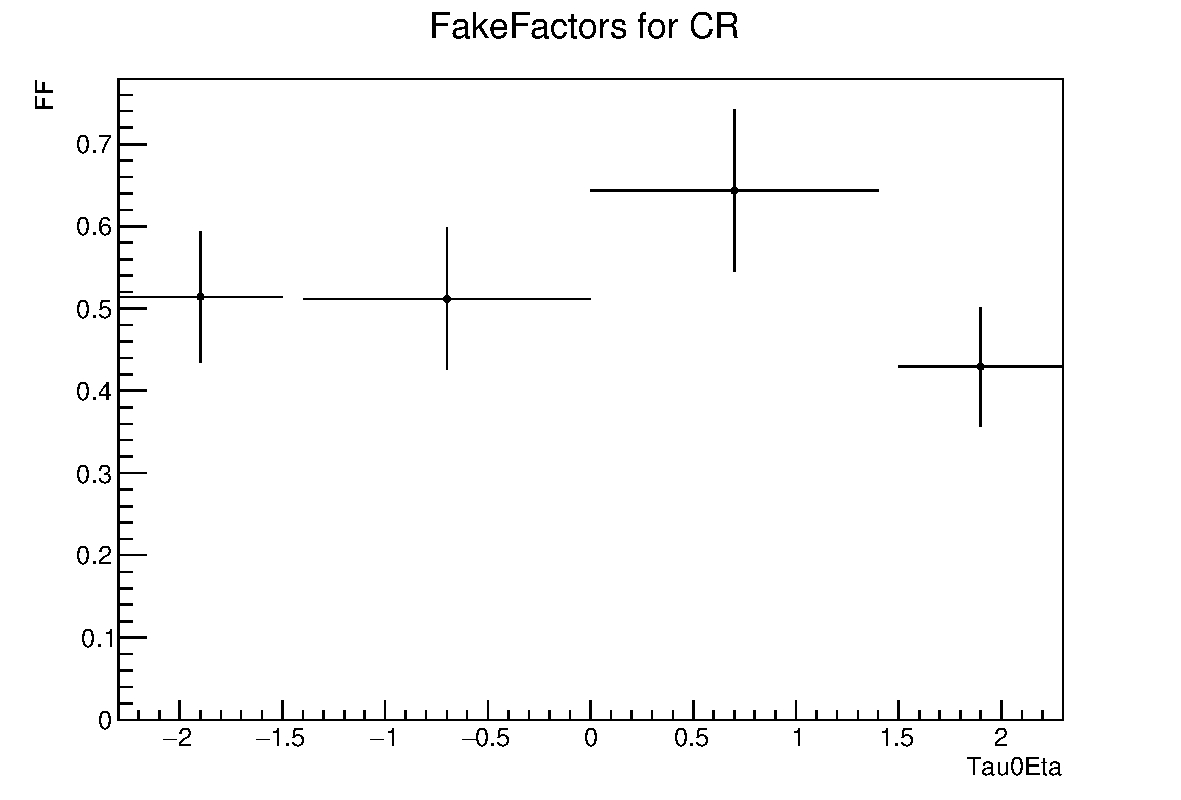
\includegraphics[width=.4\textwidth]{figures/lephadFF/LTT/FF_All_Preselection_Np1_CR_2tag_Tau0Eta}
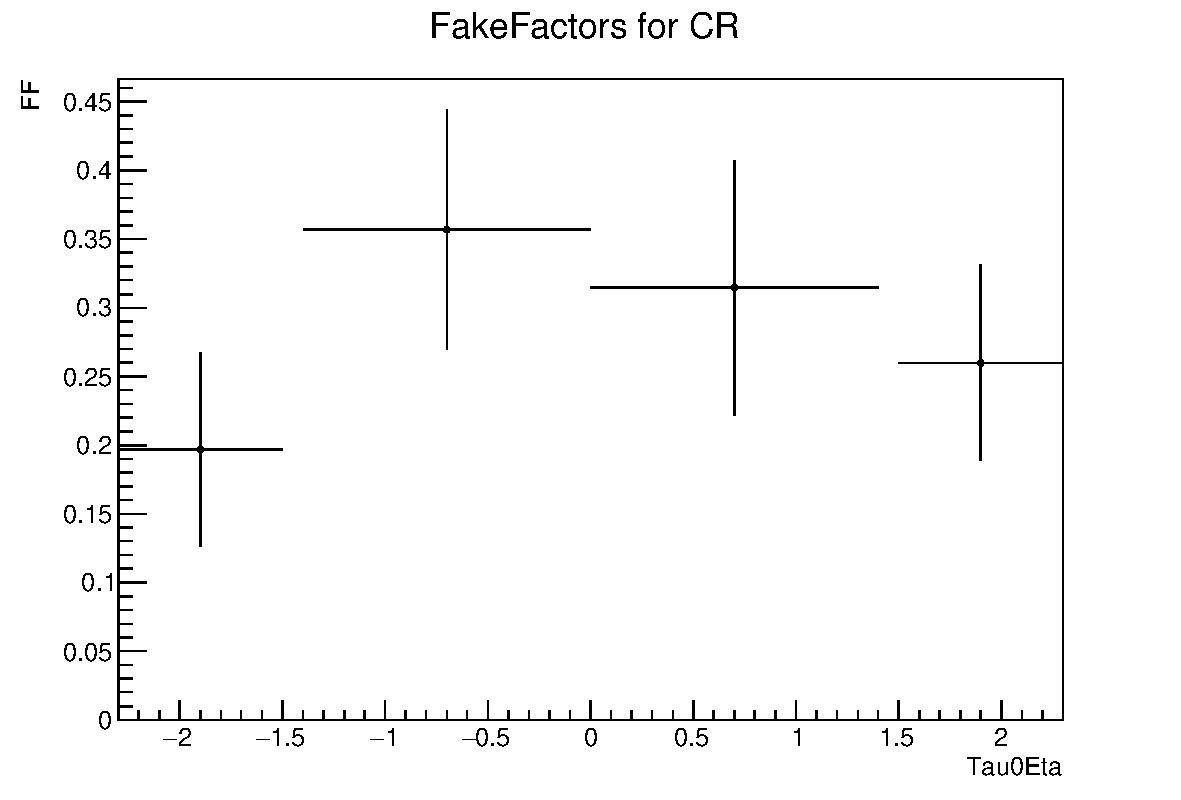
\includegraphics[width=.4\textwidth]{figures/lephadFF/LTT/FF_All_Preselection_Np3_CR_2tag_Tau0Eta} \\
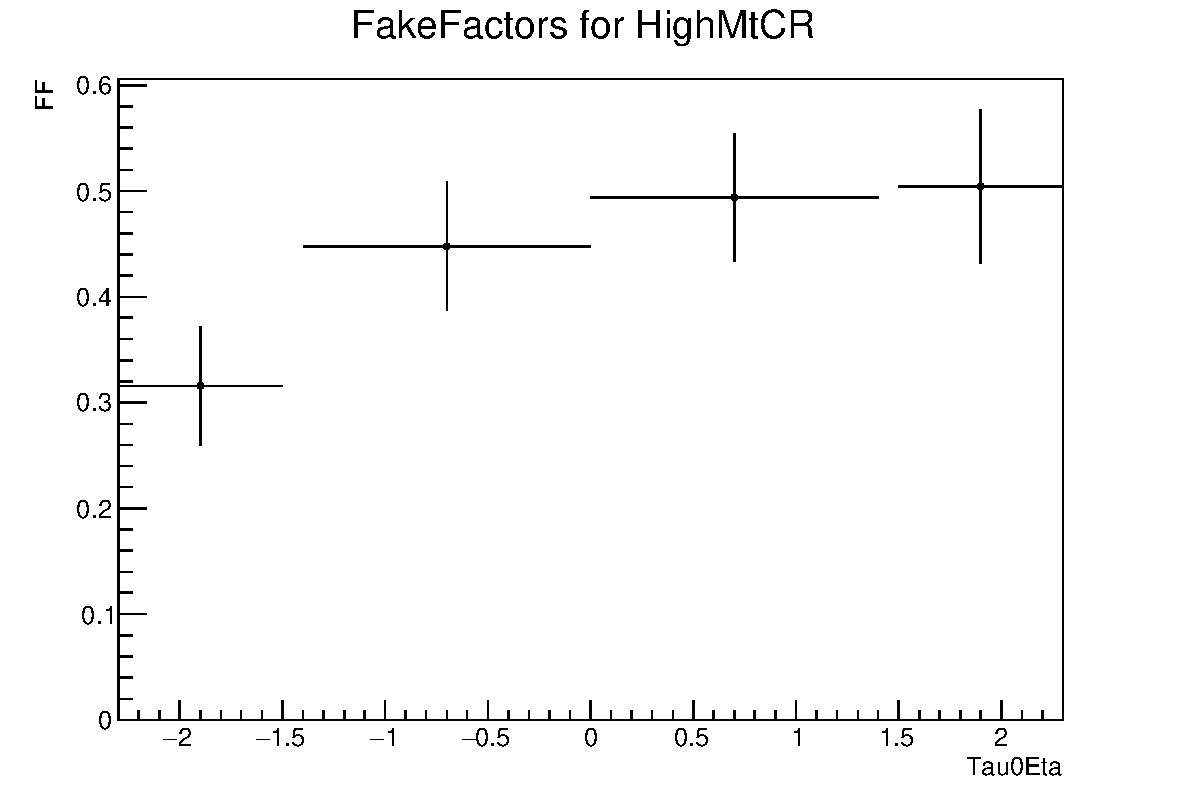
\includegraphics[width=.4\textwidth]{figures/lephadFF/LTT/FF_All_Preselection_Np1_HighMtCR_2tag_Tau0Eta}
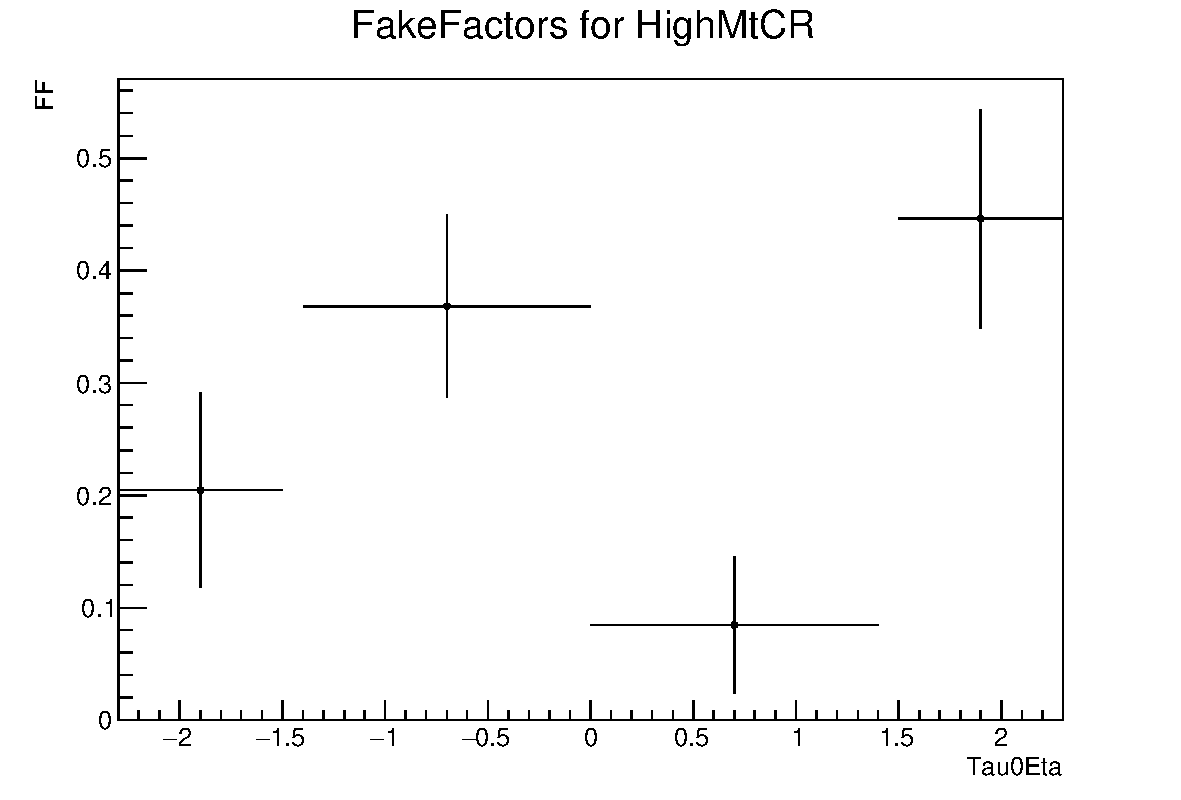
\includegraphics[width=.4\textwidth]{figures/lephadFF/LTT/FF_All_Preselection_Np3_HighMtCR_2tag_Tau0Eta}\\
\caption{Fake-factors as a function of $\eta$ for 1-prong (left) and 3-prong (right) \tauhad candidates for multi-jet (top) and \ttbar processes (bottom) for the \lephad LTT category. No significant trend is observed.}
\label{fig:lhFF_eta_LTT}
\end{figure}


Individual fake-factors for each process (multi-jet, \ttbar) are then used to provide a combined fake-factor. 
The combined $FF$ is then applied to anti-tau samples where the full signal selection is otherwise applied, 
in order to correct the normalisation and estimate the fake-\tauhad background in the regular (ID-tau) signal region. 
The combined fake-factor is defined as:

\begin{equation}
FF(\mathrm{comb}) = FF(\mathrm{QCD}) \times \mathrm{r}_{\mathrm{QCD}} + FF(\ttbar) \times (1 - \mathrm{r}_{\mathrm{QCD}}) 
\end{equation} 

where $\mathrm{r}_{\mathrm{QCD}}$ is measured as a function of the \tauhad \pT and defined as the fraction of multi-jet events in the anti-tau signal region:

\begin{equation}
\mathrm{r}_{\mathrm{QCD}} = \frac{N(\mathrm{multi\mhyphen jet, data})} {N(\mathrm{data}) - N(\mathrm{true}~\tauhad, \mathrm{MC})}
\end{equation} 

where all predicted MC events in the anti-\tauhad region are subtracted from the number of data events, $N(\mathrm{data})$, regardless of whether or not they contain a true \tauhad:

\begin{equation}
N(\mathrm{multi\mhyphen jet, data}) = N(\mathrm{data}) - N(\mathrm{true}~\tauhad, \mathrm{MC} + \mathrm{fake}~\tauhad, \mathrm{MC})
\end{equation} 

The $N(\mathrm{multi\mhyphen jet, data})$ is calculated by subtracting all background contributions apart from multi-jet, regardless of whether they contain fake or true-\tauhad candidates, from the data in the anti-ID tau region. 
The subtracted backgrounds are taken from the MC predictions. In graphical form, the various control regions where the fake factors are measured and applied can be seen in Fig.~\ref{fig:CombFFMethod}.
 
\begin{figure}
\centering
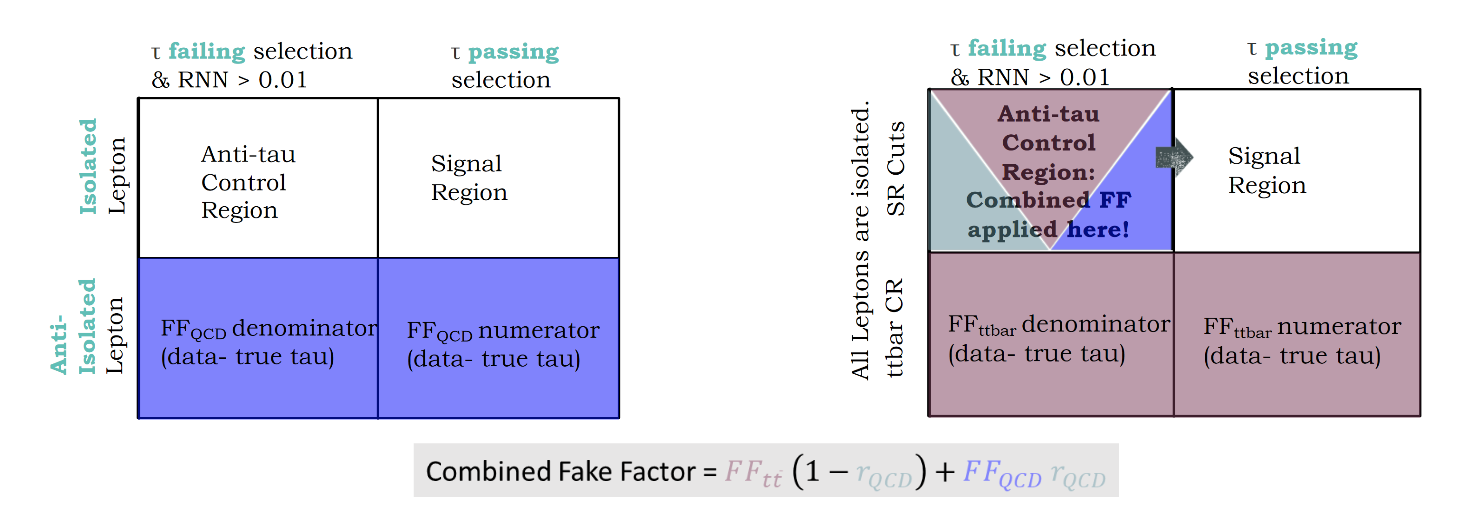
\includegraphics[width=.9\textwidth]{figures/lephadFF/CombinedFFMethod.png}
\caption{Graphical representation of the Combined Fake Factor Method}
\label{fig:CombFFMethod}
\end{figure}


It was observed that known mismodeling in the \ttbar\ background can cause issues in the calculation of the fake factors, most notably making them eventually become negative at very high values of $\tau$ transverse momentum.  For this reason, the \ttbar\ background is reweighted when it is subtracted in the calculation and application of fake factors.  This reweighting method is described in Appendix~\ref{subsec:appendix_bkg_ttbar_reweighting}.  The difference between the background estimation achieved with and without this \ttbar\ reweighting will be taken as an additional uncertainty on the method. The FF comparison with \ttbar-reweighting vs. no-\ttbar-reweighting is shown in Fig. \ref{fig:FFRW} for a demonstration of this uncertainty. This reweighting is applied in all the control regions used for the calculation of the combined fake factors, though it has the largest impact on the \ttbar fake factor contribution. 

The $\mathrm{r}_{\mathrm{QCD}}$ factor is computed both for $e\tauhad$ and $\mu\tauhad$ channels, since the QCD contents are different for them.
The parameterized $\mathrm{r}_{\mathrm{QCD}}$ as a function of \pT(\tauhad) for 1-prong and 3-prong \tauhad candidates in $e\tauhad$ and $\mu\tauhad$ channels 
are shown in Fig \ref{fig:SLT_rQCD} for the SLT category and in Fig. \ref{fig:LTT_rQCD} for the LTT category. The nature of the combined fake factor requires the same binning in both fake factors and the multi-jet fraction, but it is clear by looking at the multi-jet fraction that the \ttbar fake factor is dominant across the full $p_T$ range.  Thus, the binning of the fake factor was selected based on the \ttbar fake factor.  The binning was chosen by first looking at the fake factors as a function of $p_T$ in 5 GeV bins, and then merging statistically consistent bins until the trend was fully described. This binning is not optimal for the multi-jet fake factor and results in some binning artifact shapes at mid and high $p_T$.  As the multi-jet fake factor contributes negligibly to the combined fake factor at higher $p_T$, these binning artifacts are not seen as a significant problem.  It has been confirmed that it is possible to instead choose the binning based only on the statistics of the multi-jet fake factors, which results in a smooth trend in these fake factors.

\begin{figure}
\centering
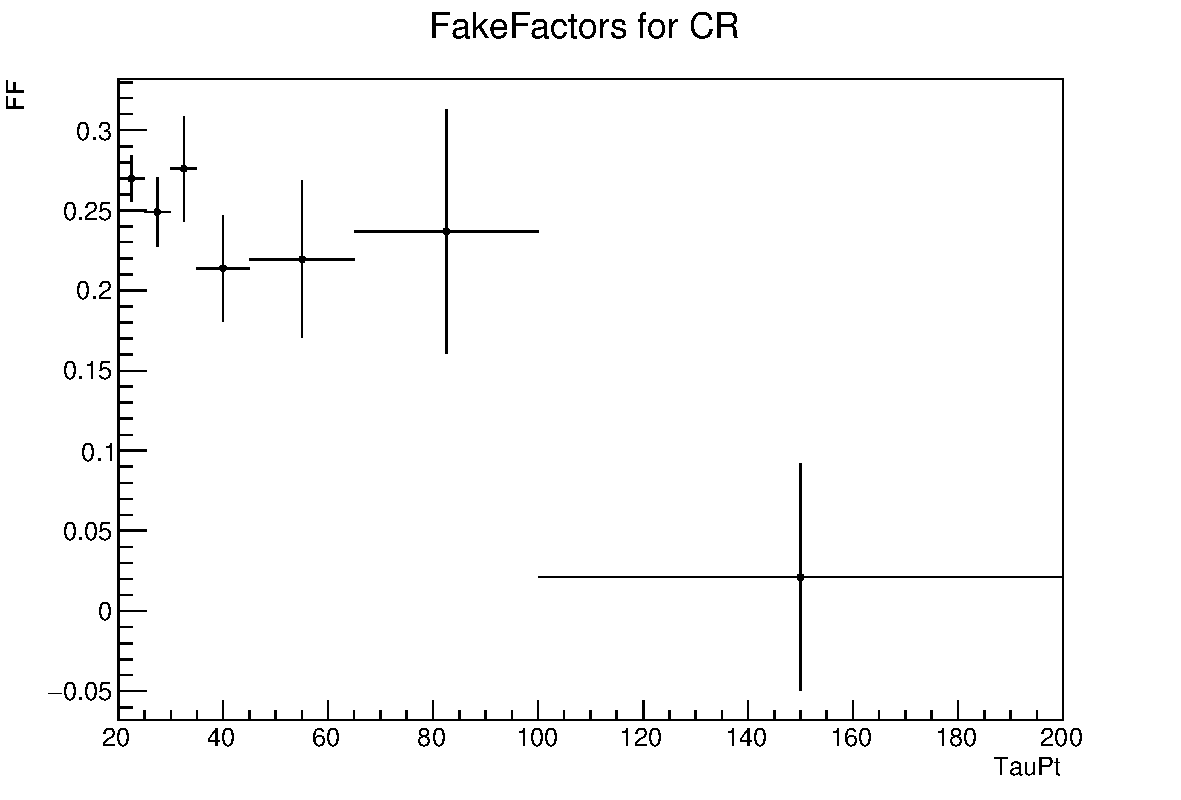
\includegraphics[width=.4\textwidth]{figures/lephadFF/SLT/FF_All_Preselection_Np1_CR_2tag_TauPt}
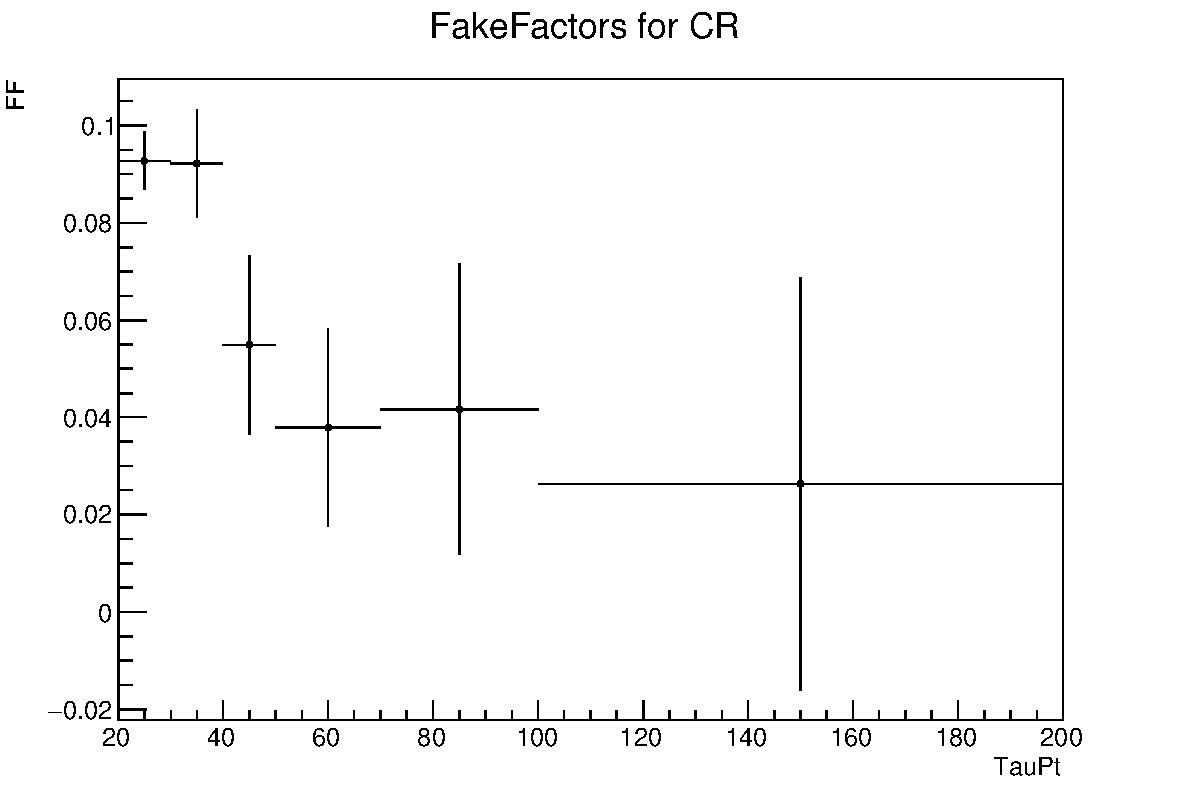
\includegraphics[width=.4\textwidth]{figures/lephadFF/SLT/FF_All_Preselection_Np3_CR_2tag_TauPt} \\
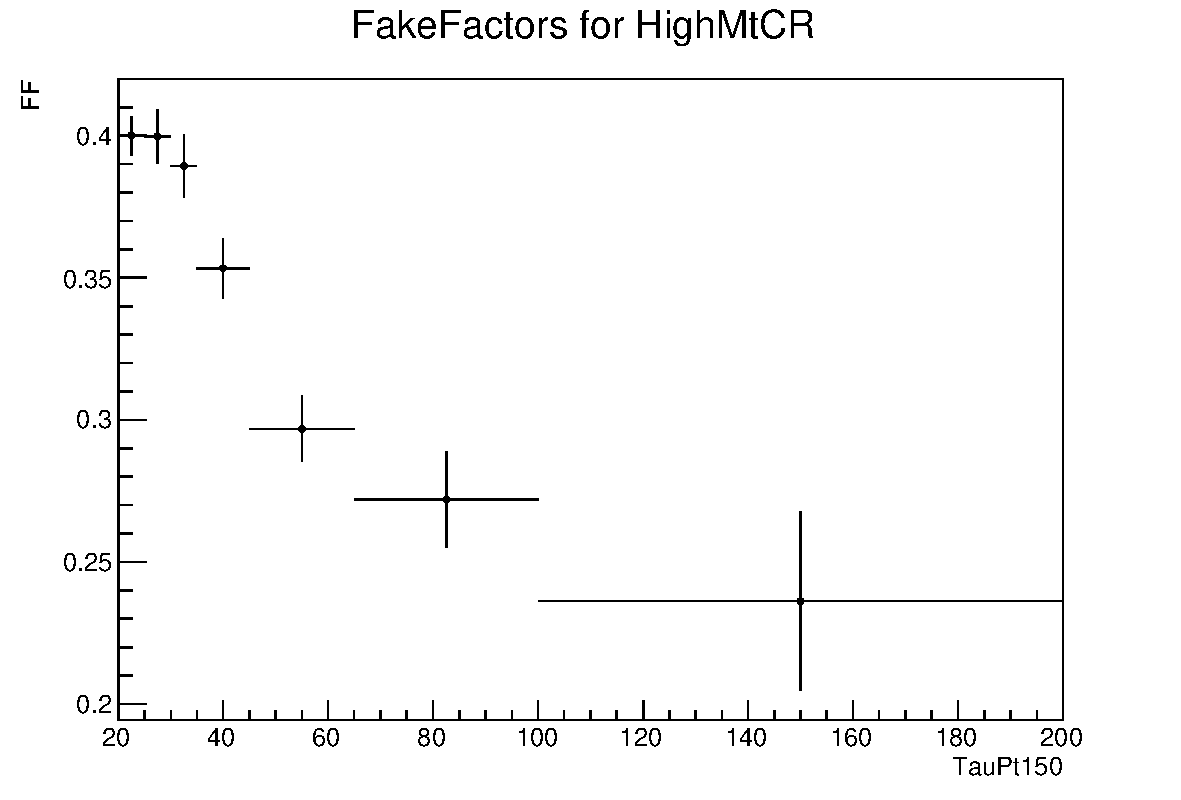
\includegraphics[width=.4\textwidth]{figures/lephadFF/SLT/FF_All_Preselection_Np1_HighMtCR_2tag_TauPt150}
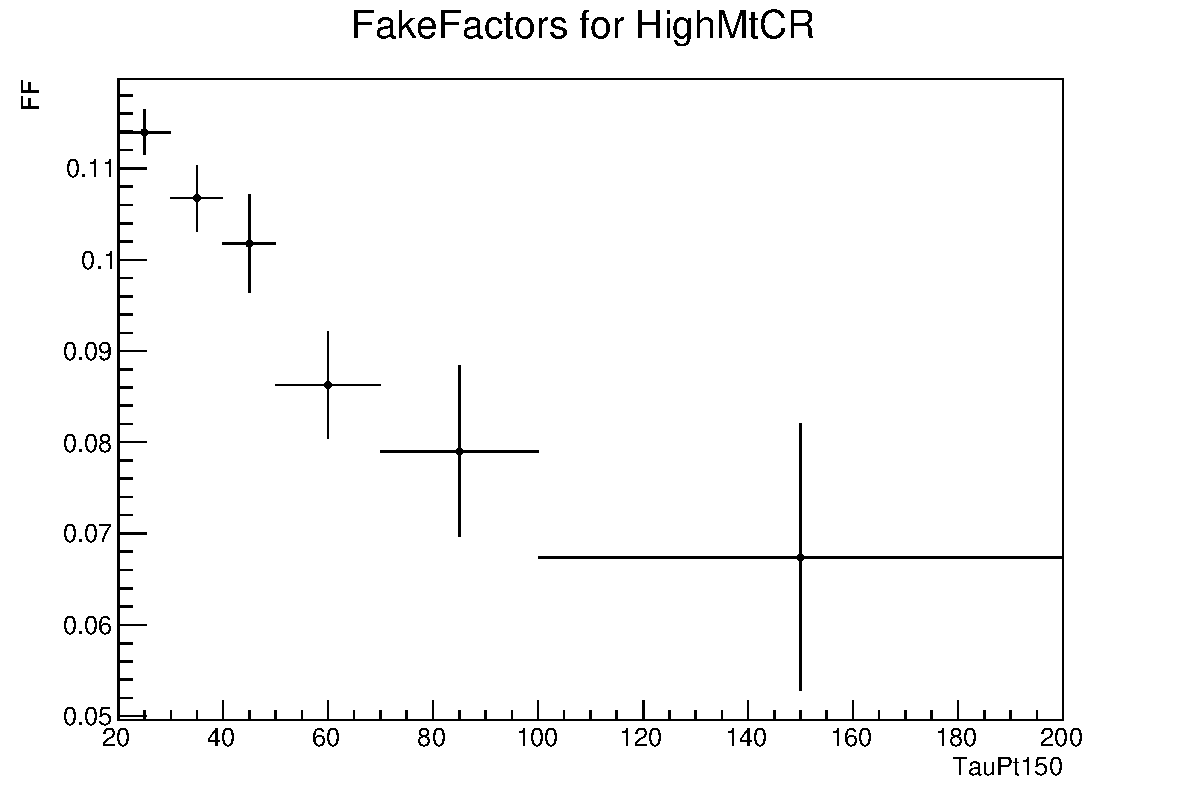
\includegraphics[width=.4\textwidth]{figures/lephadFF/SLT/FF_All_Preselection_Np3_HighMtCR_2tag_TauPt150}\\
\caption{Fake-factors for 1-prong (left) and 3-prong (right) \tauhad candidates for multi-jet (top) and \ttbar processes (bottom) for the \lephad SLT category.}
\label{fig:SLT_FF}
\end{figure}

\begin{figure}
\centering
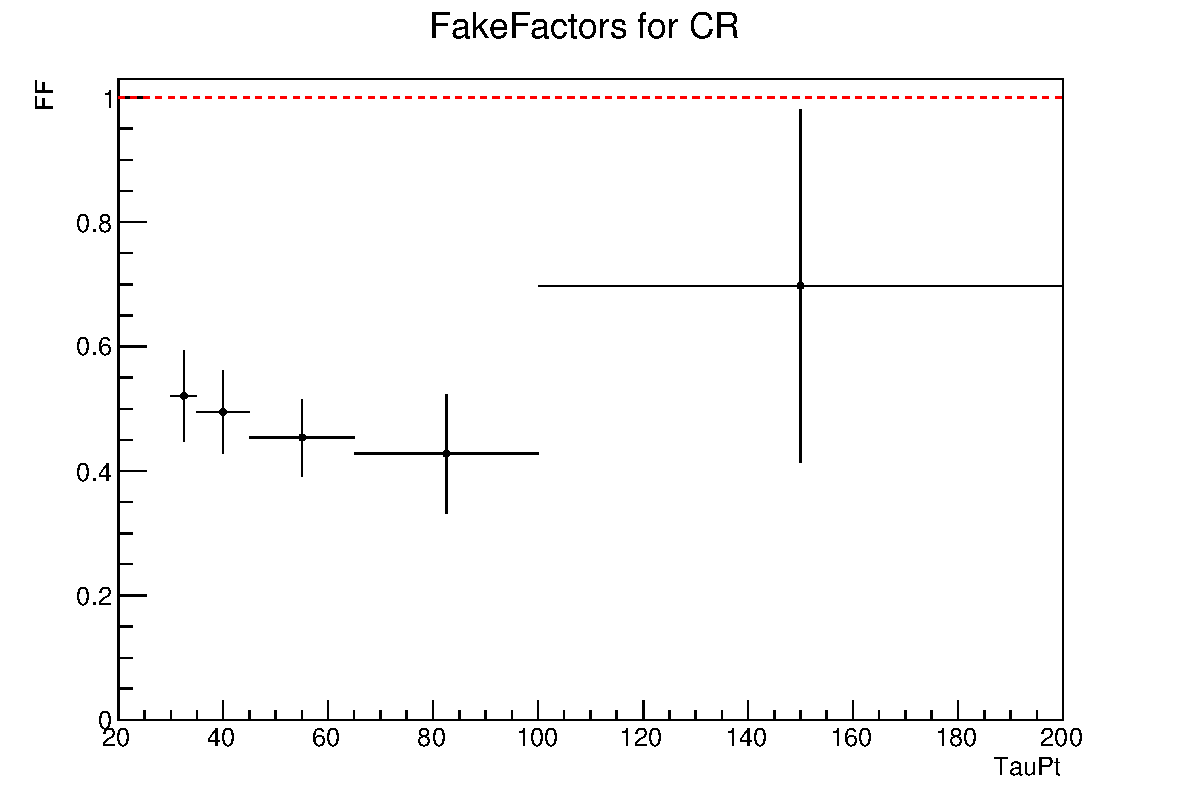
\includegraphics[width=.4\textwidth]{figures/lephadFF/LTT/FF_All_Preselection_Np1_CR_2tag_TauPt}
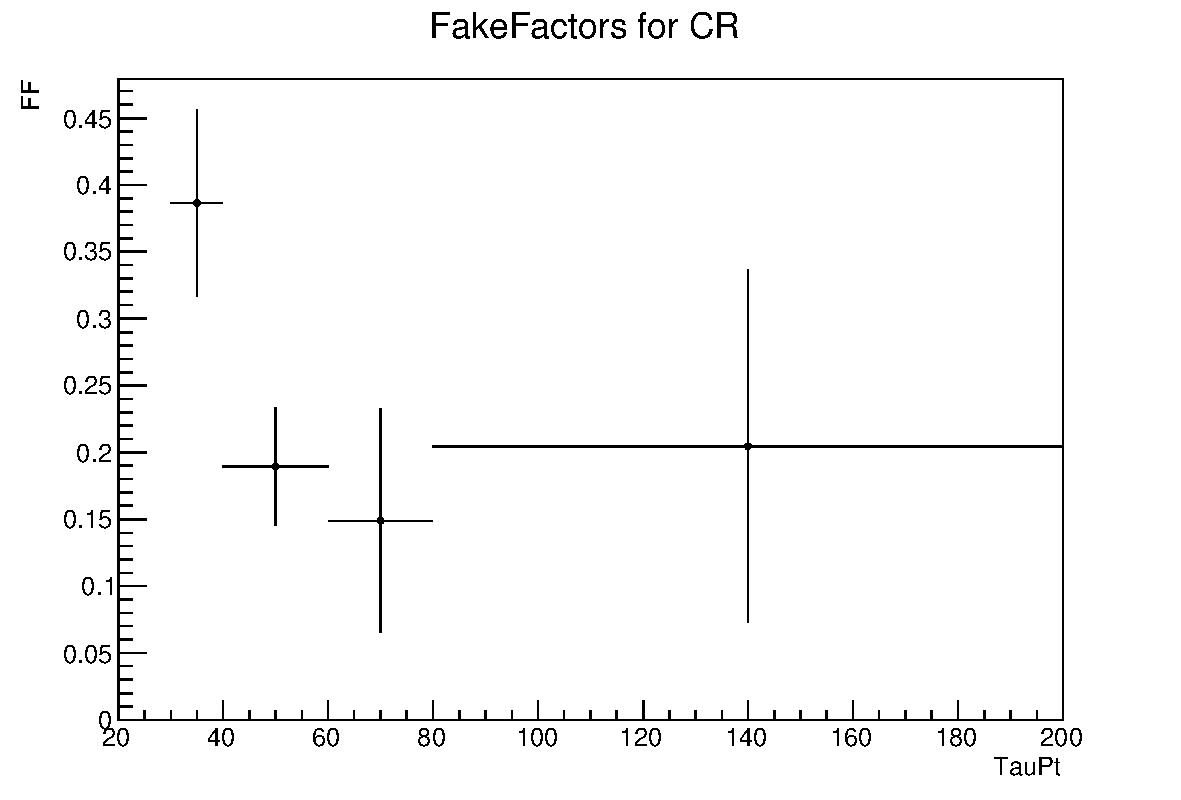
\includegraphics[width=.4\textwidth]{figures/lephadFF/LTT/FF_All_Preselection_Np3_CR_2tag_TauPt} \\
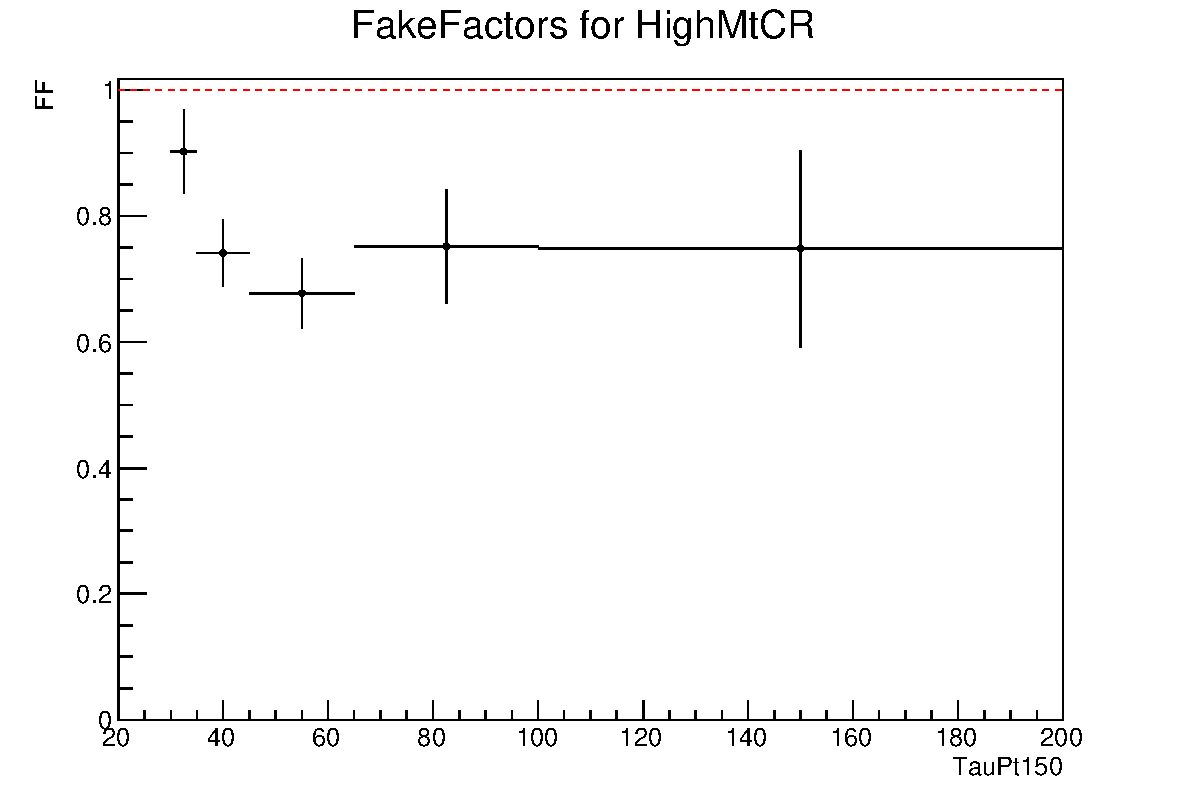
\includegraphics[width=.4\textwidth]{figures/lephadFF/LTT/FF_All_Preselection_Np1_HighMtCR_2tag_TauPt150}
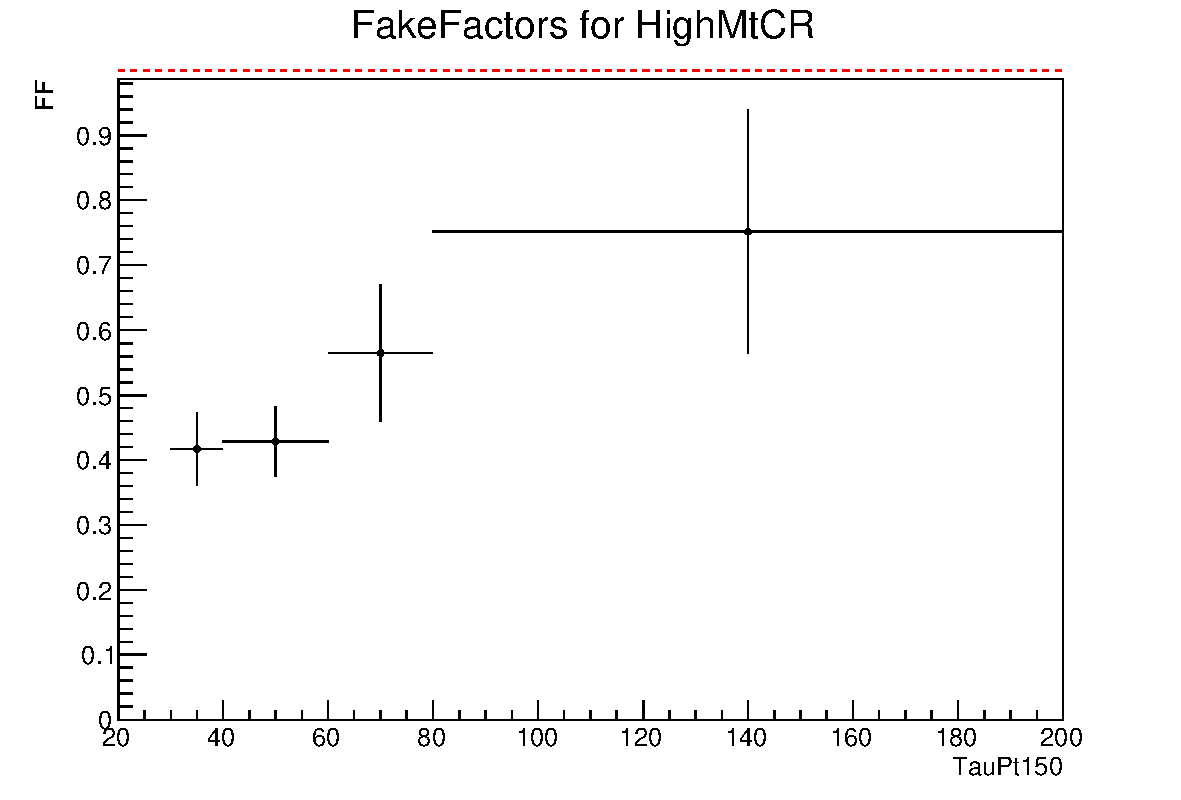
\includegraphics[width=.4\textwidth]{figures/lephadFF/LTT/FF_All_Preselection_Np3_HighMtCR_2tag_TauPt150}\\
\caption{Fake-factors for 1-prong (left) and 3-prong (right) \tauhad candidates for multi-jet (top) and \ttbar processes (bottom) for the \lephad LTT category.}
\label{fig:LTT_FF}
\end{figure}

\begin{figure}
\centering
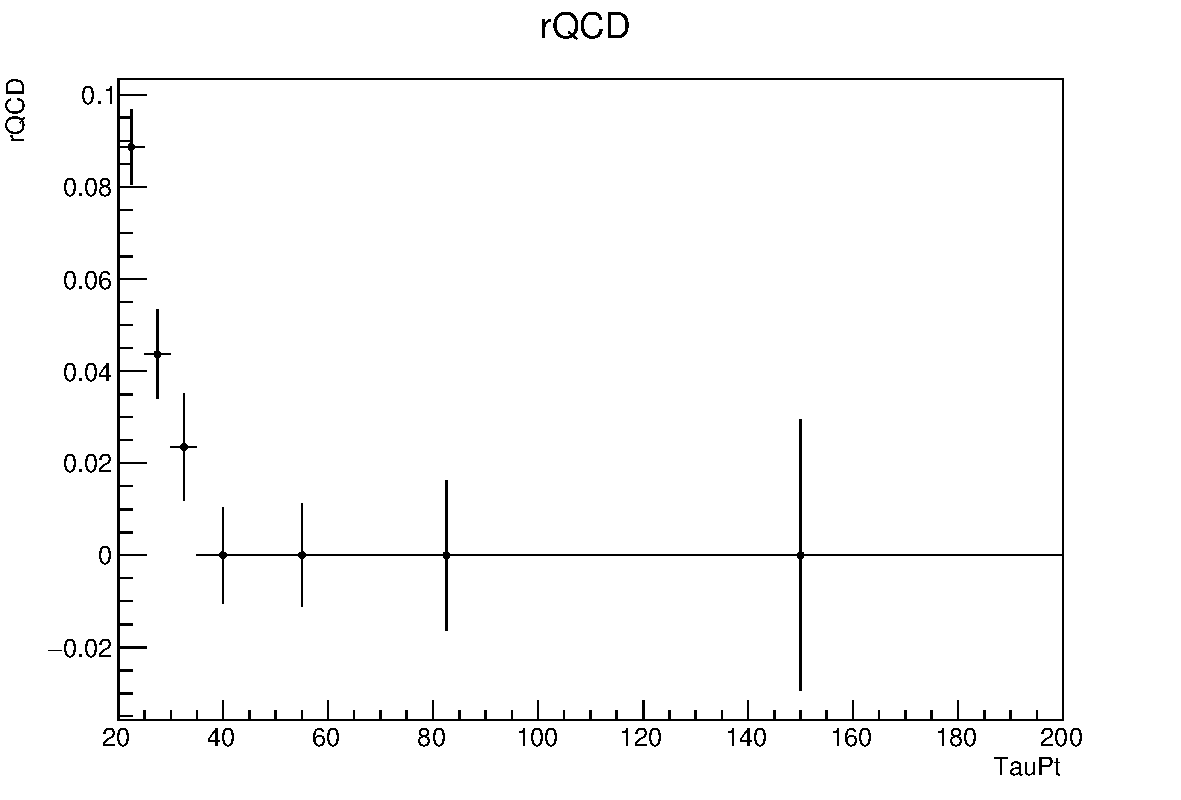
\includegraphics[width=.4\textwidth]{figures/lephadFF/SLT/rQCD_All_Preselection_Np1_Elec_CR_2tag_TauPt}
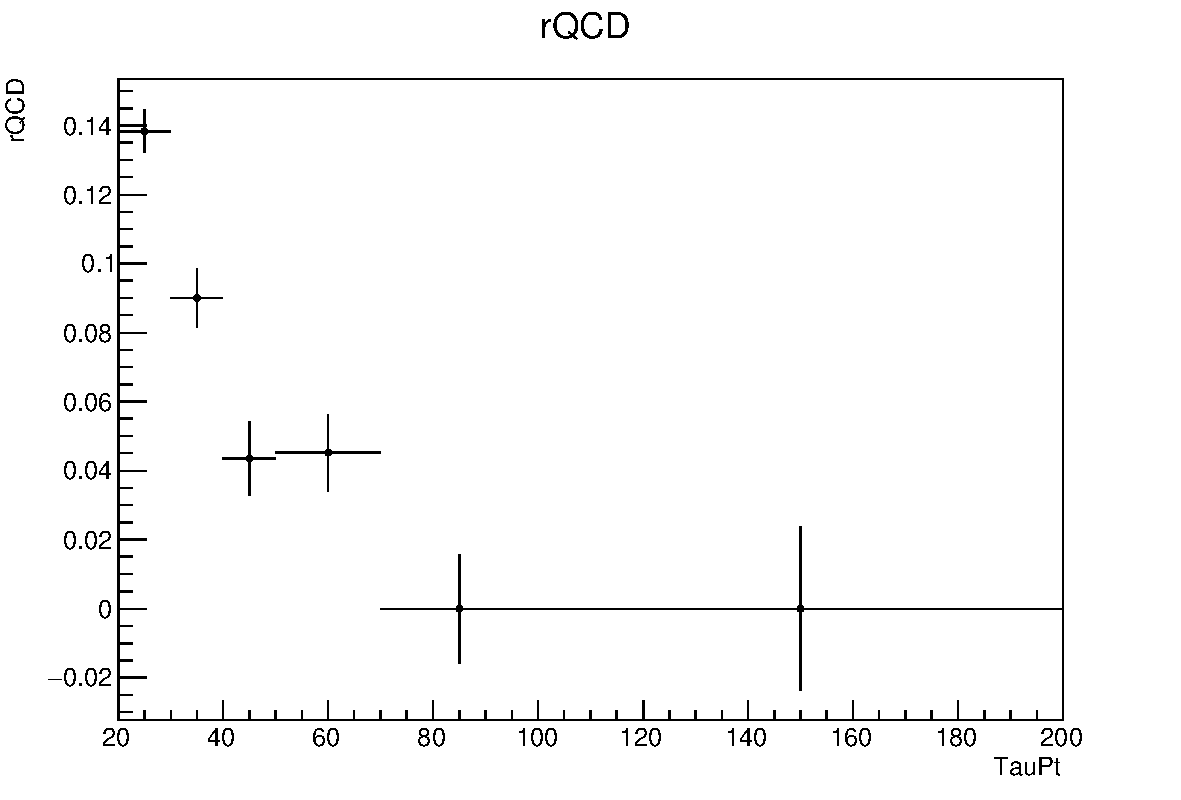
\includegraphics[width=.4\textwidth]{figures/lephadFF/SLT/rQCD_All_Preselection_Np3_Elec_CR_2tag_TauPt} \\
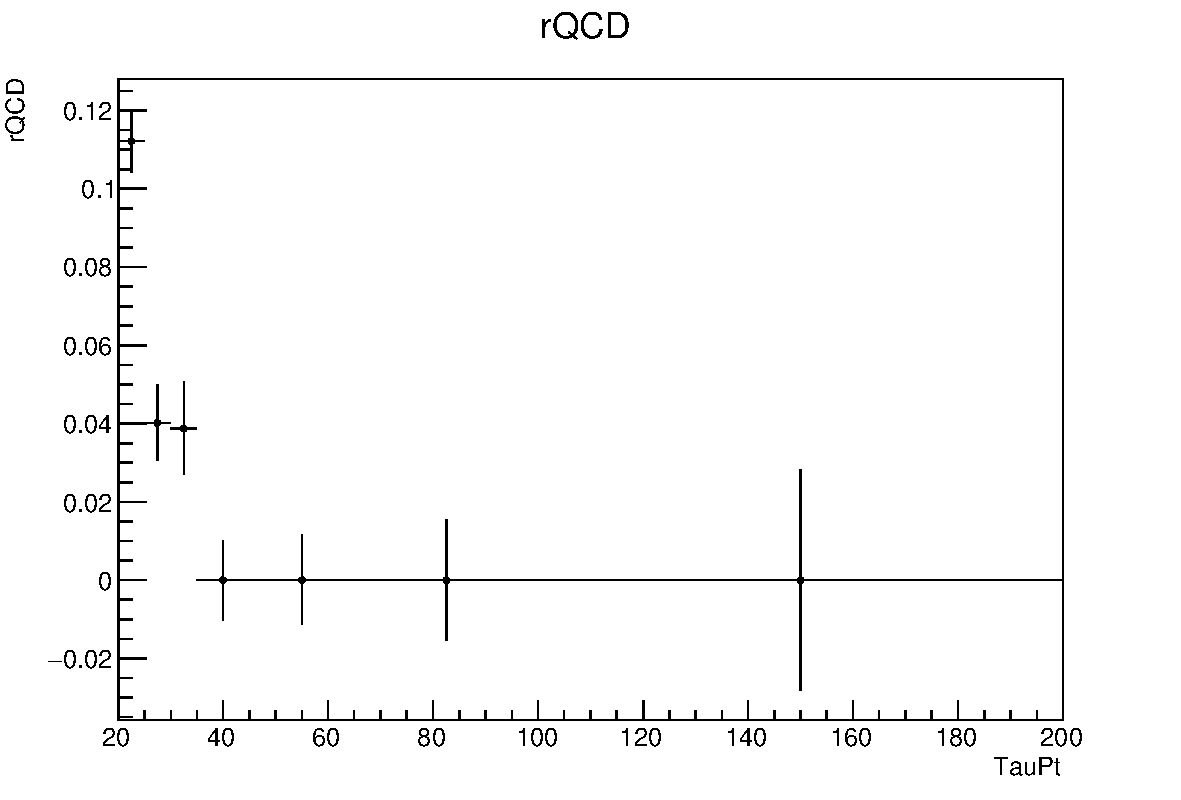
\includegraphics[width=.4\textwidth]{figures/lephadFF/SLT/rQCD_All_Preselection_Np1_Muon_CR_2tag_TauPt}
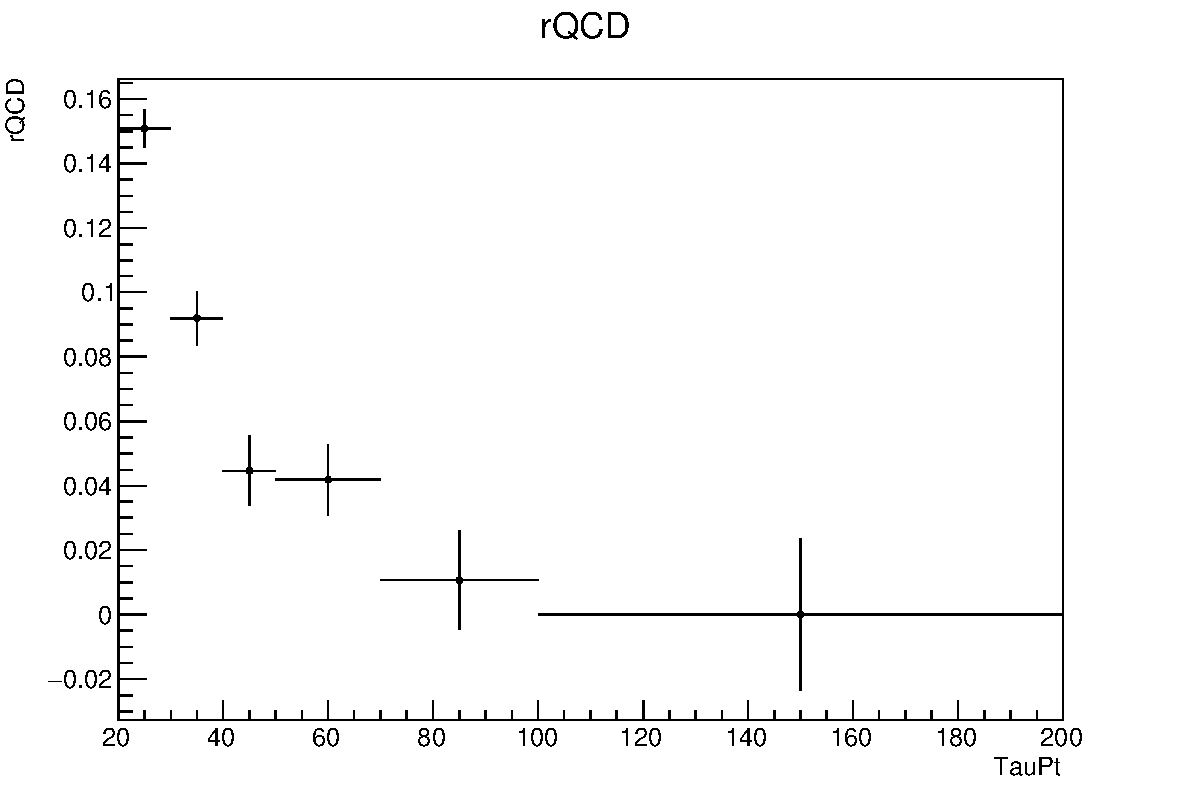
\includegraphics[width=.4\textwidth]{figures/lephadFF/SLT/rQCD_All_Preselection_Np3_Muon_CR_2tag_TauPt}\\
\caption{$\mathrm{r}_{\mathrm{QCD}}$ for 1-prong (left) and 3-prong (right) \tauhad candidates for $e\tauhad$ channel (top) and $\mu\tauhad$ (bottom) when requiring same-sign lepton-tau pairs for the \lephad SLT category.}
\label{fig:SLT_rQCD}
\end{figure}

\begin{figure}
\centering
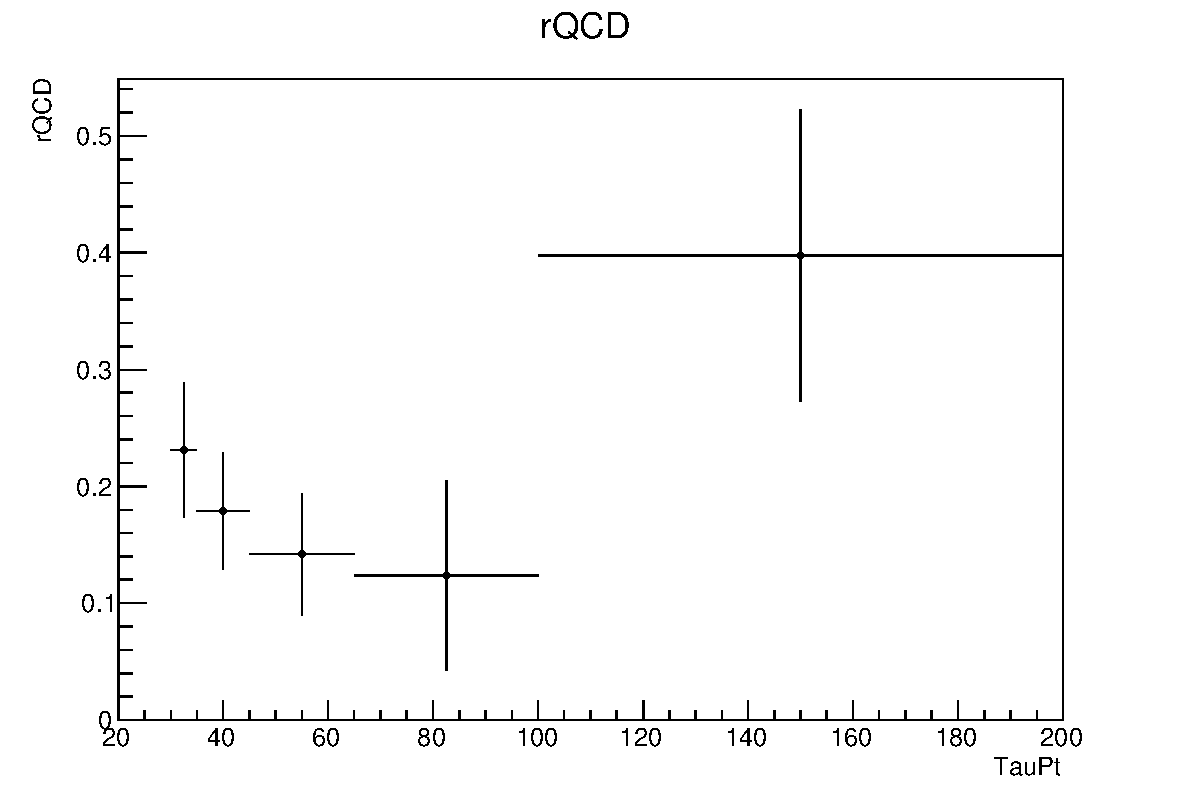
\includegraphics[width=.4\textwidth]{figures/lephadFF/LTT/rQCD_All_Preselection_Np1_Elec_CR_2tag_TauPt}
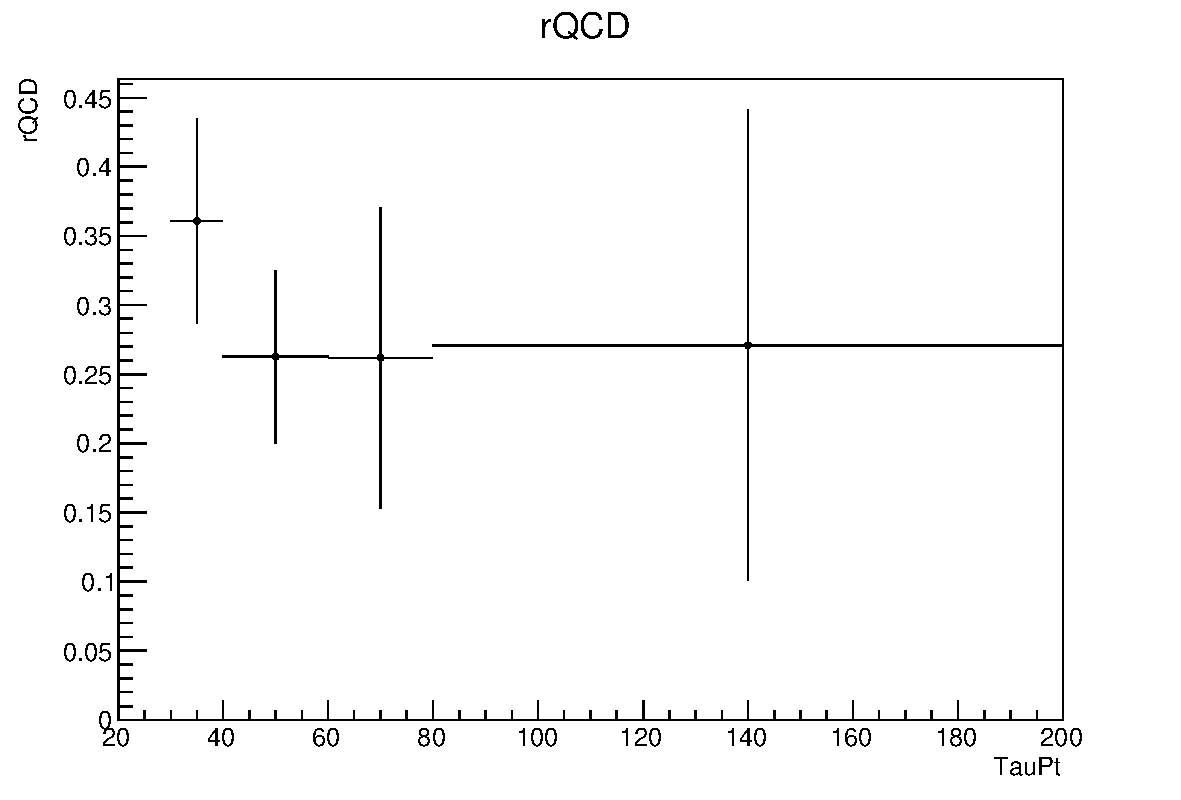
\includegraphics[width=.4\textwidth]{figures/lephadFF/LTT/rQCD_All_Preselection_Np3_Elec_CR_2tag_TauPt} \\
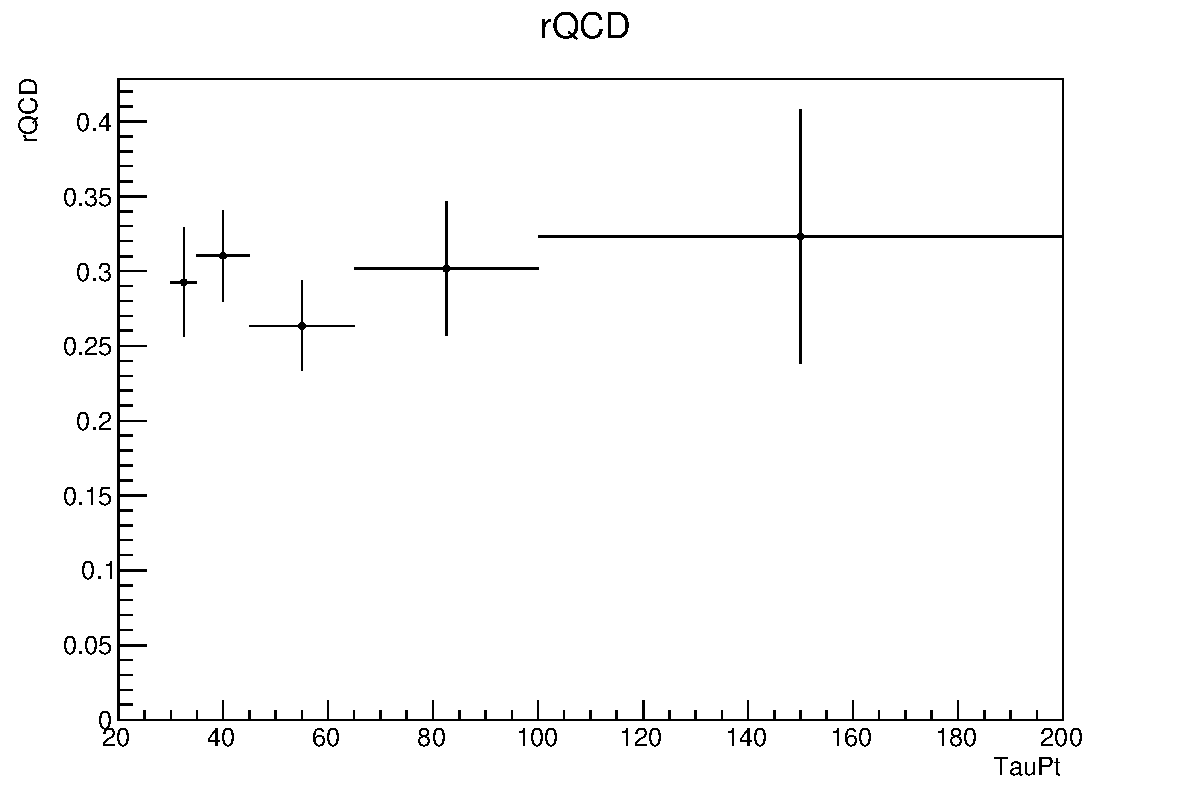
\includegraphics[width=.4\textwidth]{figures/lephadFF/LTT/rQCD_All_Preselection_Np1_Muon_CR_2tag_TauPt}
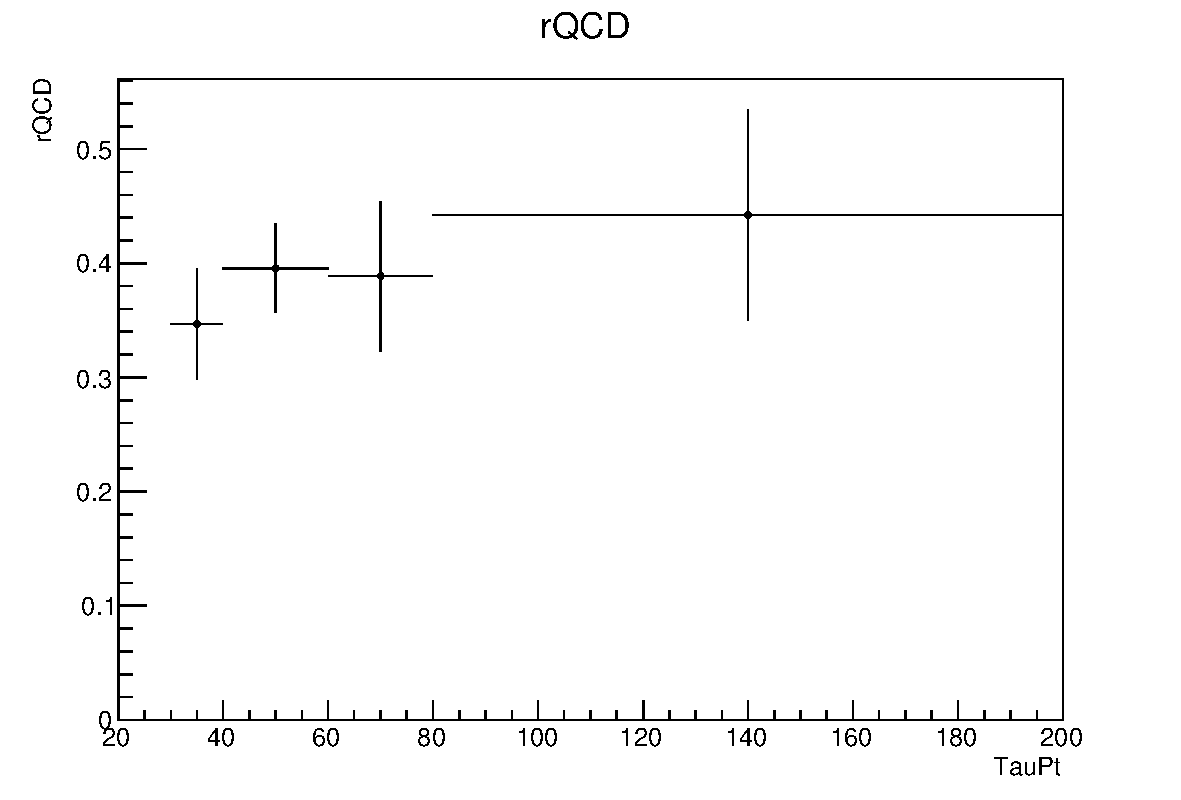
\includegraphics[width=.4\textwidth]{figures/lephadFF/LTT/rQCD_All_Preselection_Np3_Muon_CR_2tag_TauPt}\\
\caption{$\mathrm{r}_{\mathrm{QCD}}$ for 1-prong (left) and 3-prong (right) \tauhad candidates for $e\tauhad$ channel (top) and $\mu\tauhad$ (bottom) when requiring same-sign lepton-tau pairs for the \lephad LTT category.}
\label{fig:LTT_rQCD}
\end{figure}

Figure~\ref{fig:LH_MC_data_fakes} shows the comparison of the contribution of fakes as estimated using MC and using either the fake estimation or data with true $\tau$ backgrounds subtracted in the signal region and control region, respectively. As expected, the difference between MC and the data estimate is larger in the LTT channel, where the lower momentum events include more multi-jet events (for which MC is not available). This is shown with the analysis binning algorithm applied to the final discriminant for the non-resonant and several resonant mass points.

\begin{figure}
\centering
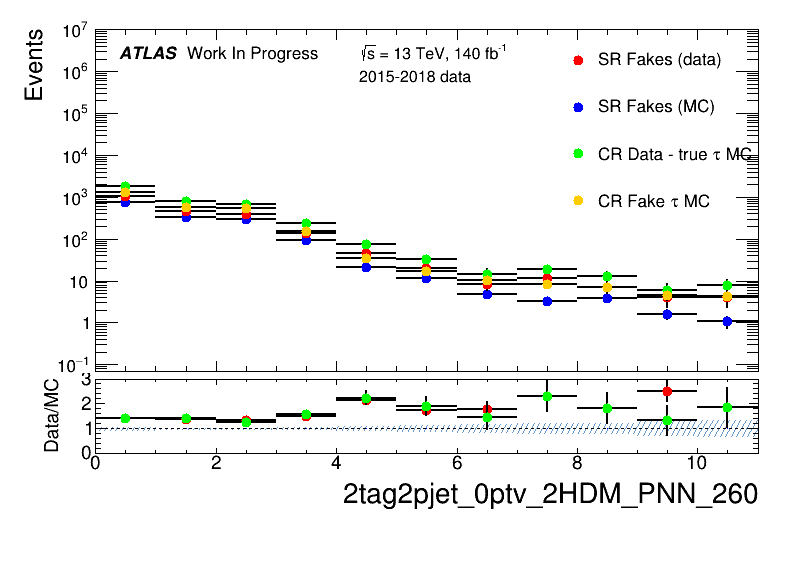
\includegraphics[width=.4\textwidth]{figures/lephadFF/LTT/2tag2pjet_0ptv_2HDM_PNN_260_LTT_CR_highPNN_fakes_log.png}
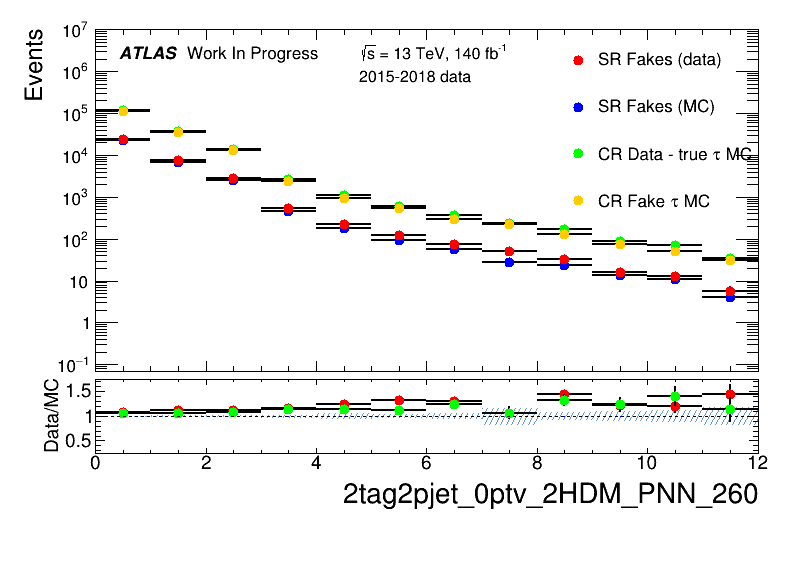
\includegraphics[width=.4\textwidth]{figures/lephadFF/SLT/2tag2pjet_0ptv_2HDM_PNN_260_SLT_CR_highPNN_fakes_log.png}\\
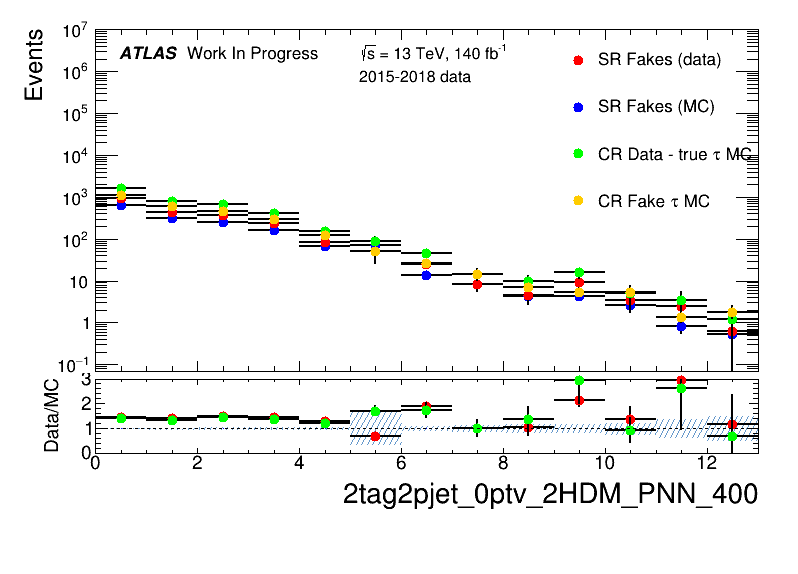
\includegraphics[width=.4\textwidth]{figures/lephadFF/LTT/2tag2pjet_0ptv_2HDM_PNN_400_LTT_CR_highPNN_fakes_log.png}
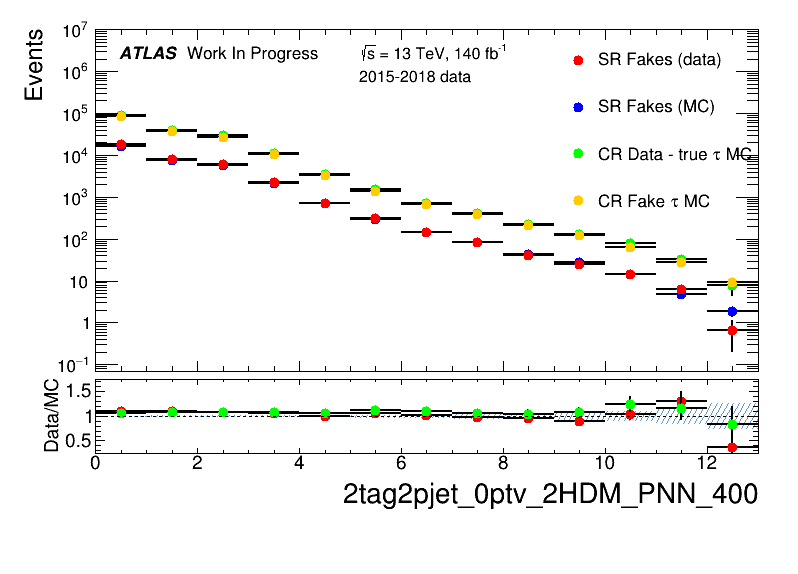
\includegraphics[width=.4\textwidth]{figures/lephadFF/SLT/2tag2pjet_0ptv_2HDM_PNN_400_SLT_CR_highPNN_fakes_log.png}\\
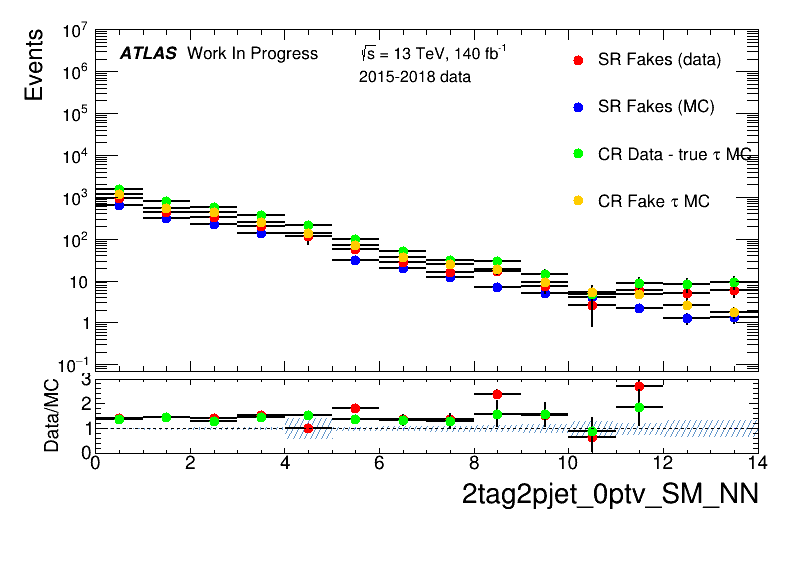
\includegraphics[width=.4\textwidth]{figures/lephadFF/LTT/2tag2pjet_0ptv_SM_NN_LTT_CR_highPNN_fakes_log.png}
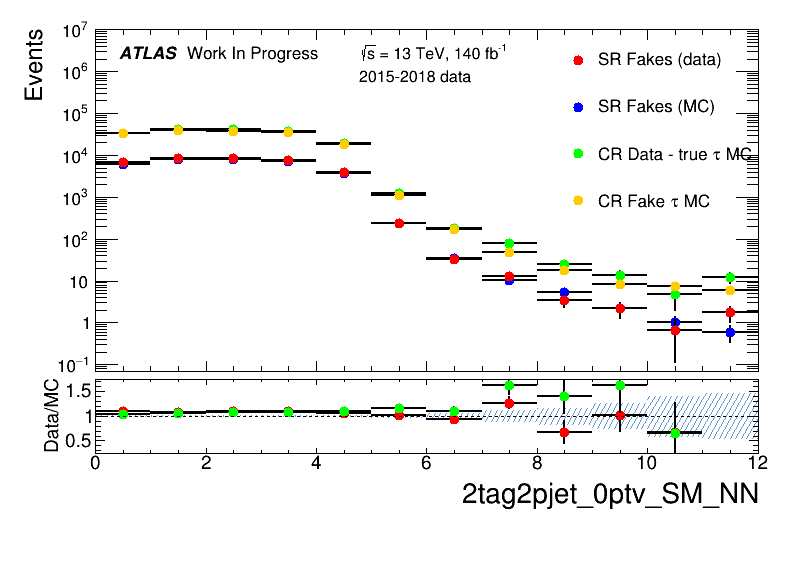
\includegraphics[width=.4\textwidth]{figures/lephadFF/SLT/2tag2pjet_0ptv_SM_NN_SLT_CR_highPNN_fakes_log.png}\\
\caption{A comparison of  the contribution of fakes as estimated using MC and using either the fake estimation or data with true $\tau$ backgrounds subtracted in the signal region and control region, respectively. Uncertainties are statistical only, and note that multi-jet contributions are included in the data estimates but not the MC. The distributions are the final discriminant for the 260 GeV (top) and 400 GeV (middle) resonant mass points, and the non-resonant discriminant (bottom) for the lepton-plus-tau trigger channel (left) and the single lepton trigger channel (right). }
\label{fig:LH_MC_data_fakes}
\end{figure} 

To validate the ability of the combined fake factor method to describe the PNN or NN shape, plots have been made using the fake factor method to estimate the combined multi-jet and $t\bar{t}/W$ contribution in validation regions. First, we have applied the combined fake factor method directly to the $\ttbar$ CR, as a closure test of the method, which can be seen in Fig.~\ref{fig:ttCR_val}. The next region is the high statistic and 
relatively background-enriched $0$-tag region, which is the same as the lephad signal region except for the requirement that there are 
no $b$-tagged jets.  This is shown in Fig.~\ref{fig:SLT_0tag} and Fig.~\ref{fig:LTT_0tag} for several mass hypotheses and for the single lepton and lepton-plus-tau trigger categories, respectively. In Fig.~\ref{fig:SLT_LTT_1tag} and Fig.~\ref{fig:SLT_LTT_1tag_NN}, a few distributions are also shown for a validation region closer to the signal region, the $1$-tag validation region, which requires the same selection as the signal region with the exception of requiring exactly one $b$-tagged jet. The background estimation appears to agree well with the observed distributions in these validation regions.

\begin{figure}
\centering
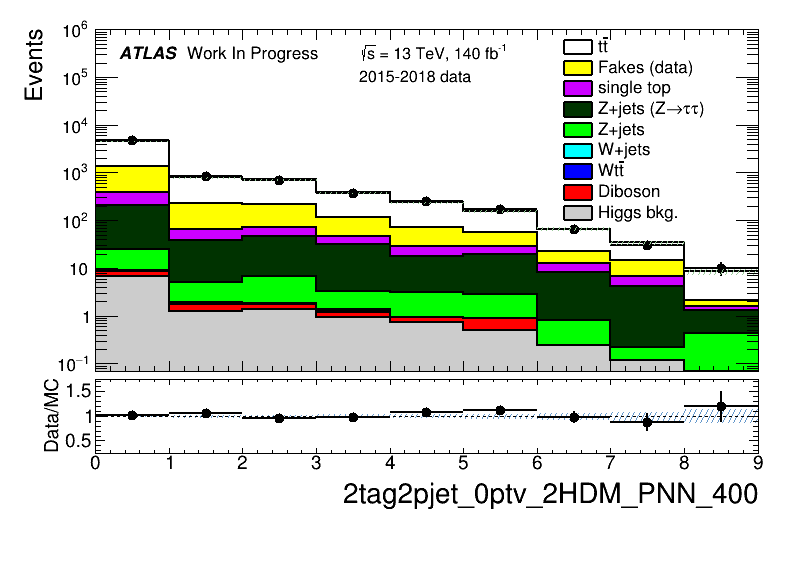
\includegraphics[width=.45\textwidth]{figures/lephadFF/LTT/2tag2pjet_0ptv_2HDM_PNN_400_SR_ALLFAKES_LTT_ttCR_noNeg_log.png}
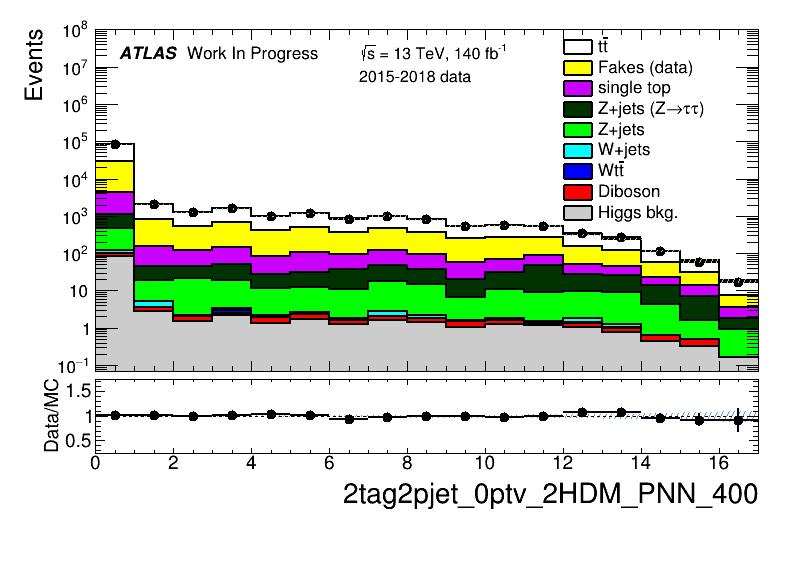
\includegraphics[width=.45\textwidth]{figures/lephadFF/SLT/2tag2pjet_0ptv_2HDM_PNN_400_SR_ALLFAKES_SLT_ttCR_noNeg_log.png}\\
\caption{The PNN distribution for the $m_{X} = 400$ GeV mass hypothesis in the signal-depleted $\ttbar$ CR where the $\ttbar$ FF are measured. This is a simple closure test.} 
\label{fig:ttCR_val}
\end{figure}



\begin{figure}
\centering
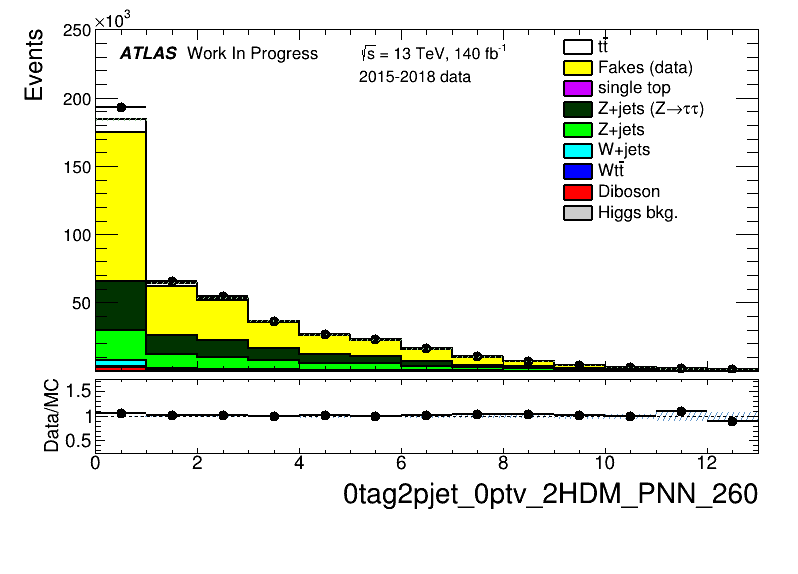
\includegraphics[width=.45\textwidth]{figures/lephadFF/SLT/0tag2pjet_0ptv_2HDM_PNN_260_SLT_ALLFAKES_Bulb_noNeg_lin.png}
\includegraphics[width=.45\textwidth]{figures/lephadFF/SLT/0tag2pjet_0ptv_2HDM_PNN_260_SLT_ALLFAKES_Bulb_noNeg_log.png}\\
\includegraphics[width=.45\textwidth]{figures/lephadFF/SLT/0tag2pjet_0ptv_2HDM_PNN_400_SLT_ALLFAKES_Bulb_noNeg_lin.png}
\includegraphics[width=.45\textwidth]{figures/lephadFF/SLT/0tag2pjet_0ptv_2HDM_PNN_400_SLT_ALLFAKES_Bulb_noNeg_log.png}\\
\includegraphics[width=.45\textwidth]{figures/lephadFF/SLT/0tag2pjet_0ptv_2HDM_PNN_1000_SLT_ALLFAKES_Bulb_noNeg_lin.png}
\includegraphics[width=.45\textwidth]{figures/lephadFF/SLT/0tag2pjet_0ptv_2HDM_PNN_1000_SLT_ALLFAKES_Bulb_noNeg_log.png}\\
\includegraphics[width=.45\textwidth]{figures/lephadFF/SLT/0tag2pjet_0ptv_SM_NN_SLT_ALLFAKES_Bulb_noNeg_lin.png}
\includegraphics[width=.45\textwidth]{figures/lephadFF/SLT/0tag2pjet_0ptv_SM_NN_SLT_ALLFAKES_Bulb_noNeg_log.png}
\caption{The PNN distribution for the $m_{X} = 260$, $400$, and $1000$ GeV mass hypotheses and the non-resonant NN distribution in the $0$-tag validation region of the single lepton trigger category in (left) linear and (right) log scale. The binning is defined using the same algorithm as is used for the signal region in the final fit, and normalization factors are used for $Z+HF$ (1.33) and $\ttbar$ (0.95).}
\label{fig:SLT_0tag}
\end{figure}    

\begin{figure}
\centering
\includegraphics[width=.45\textwidth]{figures/lephadFF/LTT/0tag2pjet_0ptv_2HDM_PNN_260_LTT_ALLFAKES_Bulb_noNeg_lin.png}
\includegraphics[width=.45\textwidth]{figures/lephadFF/LTT/0tag2pjet_0ptv_2HDM_PNN_260_LTT_ALLFAKES_Bulb_noNeg_log.png}\\
\includegraphics[width=.45\textwidth]{figures/lephadFF/LTT/0tag2pjet_0ptv_2HDM_PNN_400_LTT_ALLFAKES_Bulb_noNeg_lin.png}
\includegraphics[width=.45\textwidth]{figures/lephadFF/LTT/0tag2pjet_0ptv_2HDM_PNN_400_LTT_ALLFAKES_Bulb_noNeg_log.png}\\
\includegraphics[width=.45\textwidth]{figures/lephadFF/LTT/0tag2pjet_0ptv_2HDM_PNN_1000_LTT_ALLFAKES_Bulb_noNeg_lin.png}
\includegraphics[width=.45\textwidth]{figures/lephadFF/LTT/0tag2pjet_0ptv_2HDM_PNN_1000_LTT_ALLFAKES_Bulb_noNeg_log.png}\\
\includegraphics[width=.45\textwidth]{figures/lephadFF/LTT/0tag2pjet_0ptv_SM_NN_LTT_ALLFAKES_Bulb_noNeg_lin.png}
\includegraphics[width=.45\textwidth]{figures/lephadFF/LTT/0tag2pjet_0ptv_SM_NN_LTT_ALLFAKES_Bulb_noNeg_log.png}
\caption{The PNN distribution for the $m_{X} = 260$, $400$, and $1000$ GeV mass hypotheses and the non-resonant NN distribution in the $0$-tag validation region of the lepton-plus-tau trigger category in (left) linear and (right) log scale. The binning is defined using the same algorithm as is used for the signal region in the final fit, and normalization factors are used for $Z+HF$ (1.33) and $\ttbar$ (0.95).}
\label{fig:LTT_0tag}
\end{figure}    

\begin{figure}   
\centering
\includegraphics[width=.45\textwidth]{figures/lephadFF/SLT/1tag2pjet_0ptv_2HDM_PNN_260_SLT_ALLFAKES_Bulb_noNeg_lin.png}
\includegraphics[width=.45\textwidth]{figures/lephadFF/SLT/1tag2pjet_0ptv_2HDM_PNN_260_SLT_ALLFAKES_Bulb_noNeg_log.png}\\
\includegraphics[width=.45\textwidth]{figures/lephadFF/SLT/1tag2pjet_0ptv_2HDM_PNN_400_SLT_ALLFAKES_Bulb_noNeg_lin.png}
\includegraphics[width=.45\textwidth]{figures/lephadFF/SLT/1tag2pjet_0ptv_2HDM_PNN_400_SLT_ALLFAKES_Bulb_noNeg_log.png}\\
\includegraphics[width=.45\textwidth]{figures/lephadFF/LTT/1tag2pjet_0ptv_2HDM_PNN_260_LTT_ALLFAKES_Bulb_noNeg_lin.png}
\includegraphics[width=.45\textwidth]{figures/lephadFF/LTT/1tag2pjet_0ptv_2HDM_PNN_260_LTT_ALLFAKES_Bulb_noNeg_log.png}\\
\includegraphics[width=.45\textwidth]{figures/lephadFF/LTT/1tag2pjet_0ptv_2HDM_PNN_400_LTT_ALLFAKES_Bulb_noNeg_lin.png}
\includegraphics[width=.45\textwidth]{figures/lephadFF/LTT/1tag2pjet_0ptv_2HDM_PNN_400_LTT_ALLFAKES_Bulb_noNeg_log.png}\\
\caption{The PNN distribution for the $m_{X} = 260$ and $400$ GeV mass hypotheses in the $1$-tag validation region of the (top) single lepton trigger category and (bottom) lepton-plus-tau trigger category in (left) linear and (right) log scale. The binning is defined using the same algorithm as is used for the signal region in the final fit, and normalization factors are used for $Z+HF$ (1.33) and $\ttbar$ (0.95).}
\label{fig:SLT_LTT_1tag}
\end{figure}

\begin{figure}
\centering
\includegraphics[width=.45\textwidth]{figures/lephadFF/SLT/1tag2pjet_0ptv_SM_NN_SLT_ALLFAKES_Bulb_noNeg_lin.png}
\includegraphics[width=.45\textwidth]{figures/lephadFF/SLT/1tag2pjet_0ptv_SM_NN_SLT_ALLFAKES_Bulb_noNeg_log.png}\\
\includegraphics[width=.45\textwidth]{figures/lephadFF/LTT/1tag2pjet_0ptv_SM_NN_LTT_ALLFAKES_Bulb_noNeg_lin.png}
\includegraphics[width=.45\textwidth]{figures/lephadFF/LTT/1tag2pjet_0ptv_SM_NN_LTT_ALLFAKES_Bulb_noNeg_log.png}\\
\caption{The PNN distribution for the non-resonant signal hypothesis in the $1$-tag validation region of the (top) single lepton trigger category and (bottom) lepton-plus-tau trigger category in (left) linear and (right) log scale. The binning is defined using the same algorithm as is used for the signal region in the final fit, and normalization factors are used for $Z+HF$ (1.33) and $\ttbar$ (0.95).}
\label{fig:SLT_LTT_1tag_NN}
\end{figure}

It was also requested to see what the SM NN plots looked like in the 0-tag and 1-tag regions with the exact binning used in the signal region, rather than the a binning defined by the algorithm that is used in the signal region.  This binning is not derived from the distributions in the 0-tag and 1-tag region at all, but is instead an example of what a binning derived in a different region would look like in the validation regions.  This is shown in Fig.~\ref{fig:SLT_LTT_0tag_SR} and Fig.~\ref{fig:SLT_LTT_1tag_SR}.  

\begin{figure}
\centering
\includegraphics[width=.45\textwidth]{figures/lephadFF/SLT/0tag2pjet_0ptv_SM_NN_SLT_ALLFAKES_Bulb_SRbinning_lin.png}
\includegraphics[width=.45\textwidth]{figures/lephadFF/SLT/0tag2pjet_0ptv_SM_NN_SLT_ALLFAKES_Bulb_SRbinning_log.png}\\
\includegraphics[width=.45\textwidth]{figures/lephadFF/LTT/0tag2pjet_0ptv_SM_NN_LTT_ALLFAKES_Bulb_SRbinning_lin.png}
\includegraphics[width=.45\textwidth]{figures/lephadFF/LTT/0tag2pjet_0ptv_SM_NN_LTT_ALLFAKES_Bulb_SRbinning_log.png}\\
\caption{The NN distribution for the non-resonant signal hypothesis in the $0$-tag validation region of the (top) single lepton trigger category and (bottom) lepton-plus-tau trigger category in (left) linear and (right) log scale. The binning is exactly the same as is used for the signal region in the final fit, and normalization factors are used for $Z+HF$ (1.33) and $\ttbar$ (0.95).}
\label{fig:SLT_LTT_0tag_SR}
\end{figure}

\begin{figure}
\centering
\includegraphics[width=.45\textwidth]{figures/lephadFF/SLT/1tag2pjet_0ptv_SM_NN_SLT_ALLFAKES_Bulb_SRbinning_lin.png}
\includegraphics[width=.45\textwidth]{figures/lephadFF/SLT/1tag2pjet_0ptv_SM_NN_SLT_ALLFAKES_Bulb_SRbinning_log.png}\\
\includegraphics[width=.45\textwidth]{figures/lephadFF/LTT/1tag2pjet_0ptv_SM_NN_LTT_ALLFAKES_Bulb_SRbinning_lin.png}
\includegraphics[width=.45\textwidth]{figures/lephadFF/LTT/1tag2pjet_0ptv_SM_NN_LTT_ALLFAKES_Bulb_SRbinning_log.png}\\
\caption{The NN distribution for the non-resonant signal hypothesis in the $1$-tag validation region of the (top) single lepton trigger category and (bottom) lepton-plus-tau trigger category in (left) linear and (right) log scale. The binning is exactly the same as is used for the signal region in the final fit, and normalization factors are used for $Z+HF$ (1.33) and $\ttbar$ (0.95).}
\label{fig:SLT_LTT_1tag_SR}
\end{figure}


\FloatBarrier



\subsection{Multijet with fake-$\tau$ in the \hadhad channel}
\label{subsec:HadHadmultijet}

In the \hadhad\ channel, the multijet background is estimated using a data-driven fake-factor method, following the method used in the previous round of this analysis~\cite{HIGG-2016-16}. Fake-factors ($FF$s) are derived in a control region consisting of events with two \tauhadvis\ that have same-sign (SS) electric charges (SS CR), as ratios of the number of events with two loose \tauhad\ to the number of events with one loose and one anti-\tauhad\ candidate\footnote{Due to the skimming applied in the ``HIGG4D3'' derivations (where at least one loose \tauhad\ is required), the \tauhad-ID can be inverted only for one of the \tauhad.}. These $FF$s are applied to events with one loose and one anti-\tauhad\ candidate that have opposite-sign (OS) electric charges, in order to predict the number of OS multijet events with two loose \tauhad.

Fake-factors are derived separately for 1- and 3-prong \tauhad, separately for
the STT and DTT trigger categories, and separately for the 0-, 1- and 2-$b$-tag
regions. Moreover, the fake-factors are split by year of data-taking to account
for different \tauhad identification in the HLT and topologies being selected by
the changing trigger selection. However, due to low statistics in the SS
2-$b$-tag region, $FF$s derived in the 1-$b$-tag region are applied in the
2-$b$-tag region. For that reason, a set of transfer-factors ($TF$s) is used to
correct the multijet normalisation in the 2-$b$-tag region, as discussed below. 
The 0-$b$-tag regions are used only for validation purposes. 
The different regions used for the multijet estimation are schematically
depicted in Figure~\ref{fig:hadhadABCDMethod}. 


\begin{figure}[!h]
\centering
\captionsetup[subfigure]{justification=centering}
\subfloat[]{
\includegraphics[height=3.4cm]{figures/bkg/hadhad_multijet/FFABCD_note.pdf}
}
\subfloat[]{
\includegraphics[height=3.4cm]{figures/bkg/hadhad_multijet/FFdiagram_note.pdf}
}
        \caption{Schematic depiction of the application of the fake-factor method used to estimate the multijet background in the di-Higgs \hadhad\ channel. (\textbf{a}) Fake factors, $FF$s, are calculated in the SS region as $C/D$, after subtracting the number of simulated non-multijet events from the number of the data events in all regions. These fake-factors are then applied to the OS-region events that contain one anti-\tauhad\ candidate, region $B$, to obtain a multijet estimation in the OS region where 2 loose \tauhad\ are required, region $A$. (\textbf{b}) Fake-factors are measured separately in regions with 0, 1 and 2 $b$-tagged jets; however, fake-factors measured in the 1-$b$-tag region are applied in the 2-$b$-tag region. A set of transfer-factors, $TF$, between the 1- and 2-$b$-tag regions is derived and applied as a normalisation correction for the multijet background estimation in the 2-$b$-tag region. The 0-$b$-tag regions are used only for validation purposes.}
        \label{fig:hadhadABCDMethod}
    \end{figure}
    
    
The composition of these regions is shown in Appendix~\ref{subsec:appendix_bkg_multijetj_HadHad}. Table~\ref{tab:multijetSubtractionDTT} and Table~\ref{tab:multijetSubtractionSTT} show the relative subtraction of non-multijet-fake backgrounds in these regions.   

\begin{table}
\centering
\begin{tabular}{|c|c|c|c|}
\hline
 & 1 $b$-tag SS ID & 1 $b$-tag SS anti-ID & 2 $b$-tags OS anti-ID\\
\hline
1-prong & 12\% & 6.6\% & 54\%\\
3-prongs & 12\% & 6.8\% & 48\%\\
\hline
\end{tabular}
\caption{Relative subtraction of non-multijet-fake backgrounds in the DTT control regions used for the multijet estimation.}
\label{tab:multijetSubtractionDTT}
\end{table} 

\begin{table}
\centering
\begin{tabular}{|c|c|c|c|}
\hline
 & 1 $b$-tag SS ID & 1 $b$-tag SS anti-ID & 2 $b$-tags OS anti-ID\\
\hline
Leading \tauhad fails (1-prong) & 14\% & 3.8\% & 12\%\\
SubLeading \tauhad fails (1-prong) & 16\% & 10\% & 33\%\\
Leading \tauhad fails (3-prongs) & 20\% & 4.5\% & 18\%\\
SubLeading \tauhad fails (3-prongs) & 14\% & 12\% & 32\%\\
\hline
\end{tabular}
\caption{Relative subtraction of non-multijet-fake backgrounds in the STT control regions used for the multijet estimation.}
\label{tab:multijetSubtractionSTT}
\end{table} 
    
When only the \tauhad-ID of the $p_T$-sub-leading \tauhad\ candidate is inverted
for defining the anti-ID OS and SS CRs, a full multijet estimation is obtained.
Similarly, when only the \tauhad-ID of the $p_T$-leading \tauhad\ candidate is
inverted, another multijet estimation is obtained. To increase the number of
events that is used to model the multijet background, these two estimations are
averaged. The background templates that the fake-factors are applied to are
statistically-independent. In the STT category, due to low statistics, $FF$s are
measured inclusively in the \tauhad\ $p_T$ and $\eta$.

In the DTT category, it can be shown that the two sets of fake-factors, $FF_1$ (binned
in the $p_T$ of the sub-leading \tauhad, when only its ID is inverted) and
$FF_0$ (binned in the $p_T$ and $\eta$ of the leading \tauhad, when only its ID is
inverted), are statistically compatible (Appendix~\ref{subsec:appendix_bkg_multijetj_HadHad}: Figures~\ref{fig:app_bkg_HadHad_FFaveraging1P} and~\ref{fig:app_bkg_HadHad_FFaveraging3P}). For that reason, the fake-factors $FF_0$ and $FF_1$ are also
averaged, with taking into account the statistical significance they have in a
given $p_T$ bin\footnote{For example, $FF_0$ will not contribute to the
  inclusive fake-factor below 40~GeV, as there is a cut of 40~GeV applied to the
  leading \tauhad\ in the analysis.}. Thus, fake-factors in the DTT category,
are calculated as:

\begin{equation}
  FF_i(\pT \, \tauhad^i, \eta \, \tauhad^i, N_\text{prong} \, \tauhad^i, \dots)
  = \frac{ N_{\text{data}}(\text{loose} \, \tauhad^i)-N_{\text{non-multijet MC}}(\text{loose} \, \tauhad^i) }
  { N_{\text{data}}(\text{anti-}\tauhad^i) - N_{\text{non-multijet MC}}(\text{anti-}\tauhad^i) },
  \label{eq:HH:hadhad:multijet:FFi}
\end{equation}

where $\tauhad^i$ corresponds to the leading ($i = 0$) or subleading \tauhad ($i
= 1$) respectively. $N_{\text{data(non-multijet MC)}}$ is the number of \tauhad\
candidates in data (simulated non-multijet) events falling into the particular
$FF$ bin.

The two fake-factors, $FF_0$ and $FF_1$, are subsequently averaged using:

\begin{equation}  
  FF_\text{avg}(\pT \, \tauhad,\eta \, \tauhad, N_\text{prong} \, \tauhad, \dots) = \frac{N_{\text{data}}\text{(loose \tauhad)}-N_{\text{non-multijet MC}}\text{(loose \tauhad)}}{N_{\text{data}}\text{(anti-\tauhad)}-N_{\text{non-multijet MC}}\text{(anti-\tauhad)}},
  \label{eq:HH:hadhad:multijet:FFavg}
\end{equation}

where $N_{\text{data(non-multijet MC)}}$ in this case corresponds to the number
of \tauhad candidates in data (simulated non-multijet) events independently of
whether the \tauhadvis candidate is leading or subleading in \pT. There can be
up to two loose \tauhad\ per event in the numerator (if they are in the same
$FF$ bin), and up to one anti-\tauhad\ per event in the denominator. As already
mentioned, fake-factors defined in this way are equivalent to averaging $FF_0$
and $FF_1$, weighted by the relative number of events they contribute to a given
$p_T$ and $\eta$ bin. These fake-factors are applied to events with one anti-\tauhad, based
on its $p_T$ and $\eta$, regardless of whether this \tauhad\ is a $p_T$-leading or
sub-leading \tauhad\ in the event\footnote{The resulting multijet estimate is
  multiplied by $1/2$ effecively averaging the predictions from events where the
  leading \tauhad and the subleading \tauhad is failing identification.}. An
advantage of this approach compared to the previously-used approach with
2-dimensional fake-factor $p_T$-binning, used in the previous round of this analysis~\cite{HIGG-2016-16}, is that a finer binning can be used in
the new approach and it is easier to compare the compatibility of $FF$s between
the OS and SS regions when deriving systematic uncertainties. Nevertheless, the
two approaches give statistically compatible results, as shown in Appendix~\ref{subsec:appendix_bkg_multijetj_HadHad}: Figure~\ref{fig:app_bkg_HadHad_1Dvs2D}. Additionally, a very good agreement between the multijet estimate 
obtained when applying separately $FF_0$ and $FF_1$ to the corresponding 
events and the nominal estimate obtained when using $FF_{\mathrm{avg}}$ is 
shown in Appendix~\ref{subsec:appendix_bkg_multijetj_HadHad}: Figure~\ref{fig:app_bkg_HadHad_FFivsFFavg}.

As already mentioned, a set of transfer-factors is used to correct the
normalisation of the multijet prediction in the 2-$b$-tag region given that
fake-factors obtained in the 1-$b$-tag region are used. A transfer-factor is
defined as the ratio of the $p_T$/$\eta$-inclusive fake-factor in the 2-$b$-tag SS
region to the $p_T$/$\eta$-inclusive fake-factor in the 1-$b$-tag SS region,
inclusively derived for the STT and DTT trigger categories. Four
transfer-factors are defined, separately for 1- and 3-prong \tauhad, and
separately for the leading and the sub-leading \tauhad. The STT and DTT
fake-factors as well as the four transfer factors are given in
\Cref{fig:hadhad_fake_factors} and \Cref{fig:hadhad_transfer_factors} respectively.

\begin{figure}[h]
  \centering

  \includegraphics[width=.32\textwidth]{figures/bkg/hadhad_multijet/fake_factors/15_16/FF_1tag_TauPt_1P}
  \includegraphics[width=.32\textwidth]{figures/bkg/hadhad_multijet/fake_factors/17/FF_1tag_TauPt_1P}
  \includegraphics[width=.32\textwidth]{figures/bkg/hadhad_multijet/fake_factors/18/FF_1tag_TauPt_1P}

  \includegraphics[width=.32\textwidth]{figures/bkg/hadhad_multijet/fake_factors/15_16/FF_1tag_TauPt_3P}
  \includegraphics[width=.32\textwidth]{figures/bkg/hadhad_multijet/fake_factors/17/FF_1tag_TauPt_3P}
  \includegraphics[width=.32\textwidth]{figures/bkg/hadhad_multijet/fake_factors/18/FF_1tag_TauPt_3P}

  \includegraphics[width=.32\textwidth]{figures/bkg/hadhad_multijet/fake_factors/15_16/FF_STT_1tag}
  \includegraphics[width=.32\textwidth]{figures/bkg/hadhad_multijet/fake_factors/17/FF_STT_1tag}
  \includegraphics[width=.32\textwidth]{figures/bkg/hadhad_multijet/fake_factors/18/FF_STT_1tag}

  \caption{Fake factors for 1-prong DTT (top), 3-prong DTT (middle), and STT
    (bottom) for the data-taking periods 15-16 (left), 17 (center), and 18
    (right) for the di-Higgs \hadhad channel.}

  \label{fig:hadhad_fake_factors}
\end{figure}

\begin{figure}[h]
  \centering

  \includegraphics[width=.32\textwidth]{figures/bkg/hadhad_multijet/fake_factors/15_16/TF_1to2tag}
  \includegraphics[width=.32\textwidth]{figures/bkg/hadhad_multijet/fake_factors/17/TF_1to2tag}
  \includegraphics[width=.32\textwidth]{figures/bkg/hadhad_multijet/fake_factors/18/TF_1to2tag}

  \caption{Transfer factors for the data-taking periods 15-16 (left), 17
    (center), and 18 (right) for the di-Higgs \hadhad channel.}

  \label{fig:hadhad_transfer_factors}
\end{figure}

Validation plots are shown in Appendix~\ref{subsec:appendix_bkg_validation_hadhad}.

% Fake-factors used in the DTT category are binned in the \tahad\ \pT, while 

%\begin{itemize}
%\item “ID OS”: this is the SR, defined to contain events with two 'loose' RNN $\tau_{had}$ with opposite sign of the electric charge, as described in Section~\ref{subsec:selhh_hadhad};
%\item “ID SS”: control region where the two 'loose' RNN $\tau_{had}$ are required to have same sign electric charge instead of opposite sign;
%\item “anti-ID OS”: control region where instead of two 'loose' RNN $\tau_{had}$, one 'loose' $\tau$ and one anti-$\tau_{had}$ must be present, with anti$\tau$ defined as in Section~\ref{subsec:taus_antitaus}, and the two objects must have opposite sign electric charge;
%\item  “anti-ID SS”: control region defined as the previous region but the two objects are required to have same sign electric charge.
%\end{itemize}

%In each of the three control regions defined above the contributions from other background processes, corresponding to about 5\% of the number of data events in the region, are subtracted from the data using MC predictions. The fake-factors (FF) are then calculated from data in the ``SS'' regions as the ratio of the number of events in the ``ID SS'' region and the number of events in the ``anti-ID SS'' region:

%\begin{equation}
%FF = \frac{N^{ID}_{SS}}{N^{anti-ID}_{SS}}\,.
%\end{equation} 


%These FFs are then applied as event weights to the data events in the ``anti-ID OS'' region to obtain the estimation of QCD multi-jet events in the ``ID OS'' signal region:

%\begin{equation}
%N^{ID}_{OS}= N^{anti-ID}_{OS} \times FF\,,
%\end{equation}

%assuming that the ratio of events in the ``ID'' and ``anti-ID'' regions is the same for the ``SS'' and ``OS'' regions. In this way, multi-jet events in the opposite sign (OS) di-$\tau$ signal region are modelled with events from the anti-$\tau$ region, weighted by a fake-factor (FF). 
 
%The binning of the fake factors is dependent on the trigger that selected the
%event. For STT events the fake factor is binned in whether the anti-\tauhadvis
%is leading or subleading in \pT, and the decay mode of the \tauhadvis
%($N_\text{track}$). Due to low statistics in the STT category the fake factors
%are inclusive in \tauhadvis \pT. The \tauhadvis identification at the HLT is
%only applied to one of the two \tauhadvis candidates affecting the probability
%of jets faking \tauhadvis, motivating the binning in whether the leading /
%subleading \tauhadvis fails the identification.

%For DTT events, HLT \tauhadvis identification is applied to both \tauhadvis
%candidates. Therefore, the fake factors do not need to distinguish between cases
%where the leading and subleading \tauhadvis fails the loose identification. The
%fake factors for DTT events are parametrised in the \pT and decay mode of the
%the \tauhadvis candidate failing the identification requirement.

%Moreover, all fake factors are binned by data-taking period (${\text{2015-2016},
%  \text{2017}, \text{2018}}$) which takes into account the different triggers
%being used to select events used for the analysis.\todo{Chris: Might be changed soon}
% 
%The FFs are derived in the 1 $b$-tag region, which has larger data statistics compared to the 2 $b$-tags region.
%\textcolor{red}{To do: Chris will add info on transfer factor}


%\subsection{\ttbar with fake-\tauhad in the \hadhad channel with fake-rate method}
%\label{subsec:ttbarfake}

%In the \hadhad\ channel, the \ttbar\ background with one or two fake-\tauhad\ candidates can be estimated using a semi-data-driven fake-rate ($FR$) method, following the method used in the previous round of this analysis~\cite{HIGG-2016-16}.  

An alternative scale-factor method, described in Section~\ref{sec:ttbarfake_hadhad_sf_method}, has been developed in this round of the analysis and it is currently used for the estimation of the \ttbar\ background with one or two fake-\tauhad\ candidates.

The previously used fake-rate method is described in this appendix.

Fake-rates, per \tauhadvis, as a function of the \tauhadvis\ $p_T$, are measured in a dedicated fake-rate \ttbar\ control region ($FR$ \ttbar\ CR) defined on top of the \lephad\ SLT channel selection. These $FR$s represent probabilities for a quark- or gluon-initiated jet to fake a \tauhad\ candidate in \ttbar\ events and they are applied per selected fake-\tauhad\ to events in a specially-designed template in the \hadhad\ channel, as will be explained in the following.

Supporting material for this section can be found in Appendix~\ref{subsec:appendix_bkg_ttbarfakes}.

\subsubsection{Derivation of the fake-rates in the \lephad\ channel}

The $FR$ \ttbar\ CR is designed to select events passing a selection equivalent to the one applied to define the \lephad\ SLT channel, but without applying any \tauhad-ID requirements\footnote{In this case, there is no lower cut on the \tauhad-ID RNN score. Fake-rates are designed to model correctly the efficiency of the \tauhad-ID in simulated events. Any prior \tauhad-ID requirement when selecting the simulated events to which the $FR$s are applied would prevent the $FR$ method from fulfilling its purpose. As an example, requiring RNN score $ > 0.01$ already rejects around $3/4$ of fake-\tauhad\ candidates.}. Furthermore, events in the $FR$ \ttbar\ CR are required to have exactly two $b$-tagged jets, visible $\tau$-lepton decay products ($e/\mu$ and \tauhadvis) with opposite-sign (OS) electric charges, \mtw$ > 40$~GeV (to eliminate potential contribution from multijet events) and \mbb$ >150$~GeV (to make the $FR$ CR orthogonal to the \lephad\ SLT SR). Additionally, only events with more that 2 jets and \mtw$ < 135$~GeV are considered when measuring the fake-rates in order to increase the ratio of the number of \ttbar\ events with at least one fake-\tauhad\ to the number of \ttbar\ events with two true-\tauhad.

The defined control region has a very similar \tauhad\ origin composition as a function of the \tauhad\ \pT\ to the \hadhad\ \ttbar\ fake-\tauhad\ MC template to which the fake-rates are applied, as can be seen in Appendix~\ref{subsec:appendix_bkg_ttbarfakes}: Figure~\ref{fig:app:ttbarfake_LHvsHHcomposition}.

Given that \tauhad\ triggers are used to select events in the \hadhad\ channel, the online \tauhad-ID requirements are taken into account when deriving fake-rates\footnote{The online \tauhad-ID is usually fully efficient when applied on top of the offline \tauhad-ID for true-\tauhad; however, this is is not the case for fake-\tauhad.}. Hence, two sets of fake-rates are measured

\begin{equation}
FR        = \frac{N_{\text{data}}(\text{loose trigger-matched }\tauhad) - N_{\text{non-`\ttbar\ with fake-\tauhad' MC}}(\text{loose trigger-matched }\tauhad)}{N_{\text{data}}(\text{all }\tauhad) - N_{\text{non-`\ttbar\ with fake-\tauhad' MC}}(\text{all }\tauhad)}, \label{eq:FRDef}
\end{equation}

\begin{equation}
FR^\prime = \frac{N_{\text{data}}(\text{loose }\tauhad) - N_{\text{non-`\ttbar\ with fake-\tauhad' MC}}(\text{loose }\tauhad)}{                                N_{\text{data}}(\text{all }\tauhad) - N_{\text{non-`\ttbar\ with fake-\tauhad' MC}}(\text{all }\tauhad)}, \label{eq:FRPrimeDef}
\end{equation}

where $FR$ represents a probability for a quark- or gluon-initiated jet to pass \verb|HLT_tauXX|, where \verb|XX| is \verb|25| or \verb|35|, and to satisfy the loose offline RNN \tauhad-ID, while $FR^\prime$ represents a probability for a quark- or gluon-initiated jet to pass solely the loose offline RNN \tauhad-ID. The number ($N$) of simulated non-`\ttbar\ events with fake-\tauhad' are subtracted\footnote{There is no clear indication of the presence of multijet background in this \ttbar-enriched $FR$ CR and thus multijet is not taken into account in the subtraction. The potential missing multijet contribution was however taken into account by introducing a down-variation in the normalisation of the obtained distributions after the subtraction when estimating systematic uncertainties.} from the number of data events in both the numerator and the denominator when deriving the fake-rates. 

The fake-rates represented by Equation~\eqref{eq:FRDef} are measured separately for

\begin{itemize}
\item \verb|HLT_tauXX_medium1_tracktwo| (2015 - 2017 data-taking periods),
\item \verb|HLT_tauXX_medium1_tracktwoEF| (2018 data-taking period), and
\item a logical OR of \verb|HLT_tauXX_medium1_tracktwoEF| and \verb|HLT_tauXX_mediumRNN_tracktwoMVA| triggers (2018 data-taking, starting from Period K).
\end{itemize}

Although these triggers were pre-scaled during the data-taking\footnote{These pre-scaled single-\tauhad\ triggers are the two ``legs'' of the di-\tauhad\ trigger.}, the trigger decision is resurrected for all events in the $FR$ \ttbar\ CR when measuring the fake-rates. In all cases, fake-rates are measured as a function of the \tauhad\ $p_T$, separately for 1- and 3-prong candidates. The measured fake-rates are shown in Figure~\ref{fig:hadhadFRs}.

\begin{figure}[!h]
\centering
\captionsetup[subfigure]{justification=centering}
\subfloat[]{
\includegraphics[width=6.5cm]{figures/bkg/hadhad_ttbar_fakes/FakeRate_OS_1P_FRs_200923}
\includegraphics[width=6.5cm]{figures/bkg/hadhad_ttbar_fakes/FakeRate_OS_3P_FRs_200923}
}

\subfloat[]{
\includegraphics[width=6.5cm]{figures/bkg/hadhad_ttbar_fakes/FakeRate_OS_1P_TrigCompFRs_200923}
\includegraphics[width=6.5cm]{figures/bkg/hadhad_ttbar_fakes/FakeRate_OS_3P_TrigCompFRs_200923}
}
\caption{Fake-rates as a function of the \tauhad\ $p_T$ measured separately for 1-prong (left) and 3-prong (right) candidates. (\textbf{a}) Fake-rates accounting for the offline \tauhad-ID ($FR^\prime$, black) and fake-rates accounting for the trigger $+$ offline \tauhad-ID ($FR$), separately for HLT\_tau25 (darker blue) and HLT\_tau35 (lighter blue) triggers, in 2015 -- 2017 data. (\textbf{b}) Fake-rates corresponding to darker blue colour in the upper plots are compared to the \tauhad\ trigger configurations used to select events corresponding to the 2018 data-taking, as indicated in the legend.}
        \label{fig:hadhadFRs}
\end{figure}

Due to the large subtraction of \ttbar\ background with two true-\tauhad\ after applying the \tauhad-ID in the $FR$ \ttbar\ CR (affecting the fake-rate numerator), the fake-rates are sensitive to the modelling of the \ttbar\ background with true-\tauhad, which is taken from simulation\footnote{Mismodelling of the \ttbar\ processes has been reported by several analyses: \href{https://indico.cern.ch/event/938202/}{link}.}. For that reason, the total \ttbar\ background is re-weighted to data prior to applying the \tauhad\ trigger and the offline \tauhad-ID in order to disentangle the two effects: the mismodelling of the \ttbar\ background and the mismodelling of the \tauhad\ trigger and the offline \tauhad-ID efficiencies for simulated fake-\tauhad. This re-weighting is described in Appendix~\ref{subsec:appendix_bkg_ttbar_reweighting}.

\subsubsection{Event selection for obtaining the MC template}
In order to obtain a prediction of the \ttbar\ background with fake-\tauhad\ in the \hadhad\ channel, fake-rates are applied per fake-\tauhad\ candidate to the simulated \ttbar\ events passing a selection described in the following. The \tauhad\ trigger requirements are removed from the object and event selections given that they are modelled by the fake-rates themselves. As already discussed, the lower cut on the \tauhad-ID RNN score is omitted.

Only events with exactly one or two loose \tauhad\ candidates are selected due to the skimming applied in the ``HIGG4D3'' derivations (where at least one loose \tauhad\ is required). Events with more than two loose \tauhad\ are rejected, following the nominal selection. Events with two loose \tauhad\ are assigned to the STT category if one of the \tauhad\ has a $p_T$ greater than the corresponding offline STT $p_T$ threshold, listed in Section~\ref{subsec:selhh_hadhad}. Otherwise, the event is assigned to the DTT category if $p_T>40\text{ }(30)$~GeV for the leading (sub-leading) \tauhad. Events with one loose \tauhad\ are considered only if they have at least one additional reconstructed \tauhad. An event is assigned to the STT category if it contains a \tauhad\ candidate (no \tauhad-ID requirements taken into account) with a $p_T$ greater than the STT threshold. The event is further required to have two \tauhad\ with $p_T>\text{STT threshold }(20)$~GeV for the leading (sub-leading) candidate, where one has to pass the loose \tauhad-ID. If an event contains more \tauhad\ candidates, one such combination is chosen randomly. If the event does not contain a \tauhad\ with a $p_T$ greater than the STT threshold, it is considered for the DTT category, where two \tauhad\ with $p_T>40\text{ }(30)$~GeV for the leading (sub-leading) candidate are required and where one of these \tauhad\ is required to pass the loose offline \tauhad-ID. If an event contains more \tauhad\ candidates, one such combination is chosen randomly. After this categorisation, events are required to pass the nominal selection criteria applied in the \hadhad\ channel (for the opposite-sign 2-$b$-tag region), with the exception of the trigger and \tauhad-ID requirements, as explained above.

The selection described here is designed to mimic the nominal event selection in the \hadhad\ channel, but without taking into account the \tauhad\ trigger decision and the offline \tauhad-ID, which are modelled by the fake-rates. The problem with the ``HIGG4D3'' skim is circumvented by introducing simulation-to-data scale-factors for events where both \tauhad\ are fake, as will be explained in the following.

\subsubsection{Application of the fake-rates}
Fake-rates are applied per fake-\tauhad\ in the MC template, obtained as discussed above. Events with two true-\tauhad\ are not considered since the \ttbar\ background with true \tauhad\ is estimated separately by applying the trigger and the \tauhad-ID requirements directly to simulated events.

The remaining events in the template can be categorised into three groups:
\begin{itemize}
\item FT -- the leading (sub-leading) \tauhad\ is fake (true);
\item TF -- the leading (sub-leading) \tauhad\ is true (fake);
\item FF -- both \tauhad\ are fake.
\end{itemize}
In the first two categories, TF and FT, the true-\tauhad\ is required to pass the loose \tauhad-ID and to be trigger-matched to a resurrected \verb|HLT_tau35(25)|, if it is the leading (sub-leading) selected \tauhad. The corresponding fake-rate is applied to the fake-\tauhad. In the DTT category and for the leading \tauhad\ in the STT category, fake-rates obtained using Equation~\eqref{eq:FRDef} are used in order to model the efficiencies of the trigger and the offline \tauhad-ID. Fake-rates obtained using Equation~\eqref{eq:FRPrimeDef} are applied to the sub-leading \tauhad\ in the STT category, as they do not account for the \tauhad\ trigger, which is not required in that case.

Events in the FF category, i.e. events with two fake-\tauhad, cannot be estimated by directly applying the fake-rates to both \tauhad, since one of them is already required to pass the loose \tauhad-ID, as explained above. For that reason, a separate set of scale-factors ($SF$s) are derived as ratios of the fake-rates in data to the fake-rates in simulated events. These scale-factors, $SF=FR/FR_{\mathrm{MC}}$ ($SF^{\prime} =FR^{\prime} /FR^{\prime}_{\mathrm{MC}}$), are then applied to events containing a loose and trigger-matched (loose) \tauhad\ in the FF category. If both candidates pass the loose \tauhad-ID, a random choice is made to which one the scale-factor is applied. The corresponding fake-rate is in both cases applied to the other \tauhad\ candidate. 

The application of fake-rates is schematically depicted in Figure~\ref{fig:FRMethodDiagram}. The modelling of the $p_T$ of the leading and sub-leading \tauhad\ candidates, in a \ttbar-enriched validation region, is shown in Figure~\ref{fig:hadhadFRMethodTauPtModelling}. Additional modelling plots are shown in Appendix~\ref{subsec:appendix_bkg_ttbarfakes}.

\begin{figure}[!h]
\centering
\includegraphics[width=10.0cm]{figures/bkg/hadhad_ttbar_fakes/FR_application.pdf}
     \caption{Schematic depiction of the application of the fake-rate method in the di-Higgs \hadhad channel. Fake-rates are applied to fake-\tauhad\ based on their $p_T$, while taking into account if the selected \tauhad\ candidate would have been required to be trigger-matched in order to pass the \hadhad\ SR selection ($FR$), or not ($FR^\prime$). True-\tauhad\ corresponding to the DTT category and the leading \tauhad\ candidate in the STT category are required to be trigger-matched to HLT\_tau35(25) for the leading (sub-leading) candidate. All true-\tauhad\ are required to pass the offline loose \tauhad-ID. For the events in the FF category, the product of a fake-rate ($FR$ or $FR^\prime$) and a scale-factor ($SF$ or $SF^\prime$) is applied given that one of the fake-\tauhad\ is already required to pass the loose \tauhad-ID. Candidates to which $SF$s ($SF^{\prime}$s) are applied are required to pass the loose \tauhad-ID and to be trigger-matched (to pass the loose \tauhad-ID).}      
       \label{fig:FRMethodDiagram}
\end{figure}

\begin{figure}[!h]
\centering
\includegraphics[width=6.5cm]{figures/bkg/hadhad_ttbar_fakes/HadHad_TopVR/TopVR1_2tag2pjet_0ptv_LL_OS_Tau0Pt.pdf}
\includegraphics[width=6.5cm]{figures/bkg/hadhad_ttbar_fakes/HadHad_TopVR/TopVR1_2tag2pjet_0ptv_LL_OS_Tau1Pt.pdf}
\caption{Pre-fit modelling of the $p_T$ of the leading (left) and sub-leading (right) \tauhad\ candidates in the di-Higgs \hadhad-channel \ttbar-enriched validation region: OS 2-$b$-tag $+$ \mbb$ >150$~GeV and $\mMMC_{\tau\tau}>150$~GeV.}
        \label{fig:hadhadFRMethodTauPtModelling}
\end{figure}

\subsubsection{Uncertainties on \ttbar with fake-$\tau$ in the $\tauhad\tauhad$-channel}

The following sources of systematic uncertainties are considered when deriving
the fake rates for the estimation of \ttbar with fake \tauhad in the
$\tauhad\tauhad$ channel: \ttbar normalisation, \ttbar reweighting, non-closure
in \tauhad \pT in the FR measurement region without \tauhad-identification, fake
rate statistical uncertainty, single top and subtraction of other backgrounds. A
summary of the uncertainty sources and their impact on the overall normalisation
is shown in~\Cref{tab:ttbarfakes_hadhad_systnorms}. The full shape information
of these sources is considered in the fit. In the following, the sources of
uncertainties are discussed individually.

\begin{table}[htb]
  \centering
  \begin{tabular}[htb]{lrrr}
    \toprule
    Uncertainty source & ttbarTF & ttbarFT & ttbarFF \\
    \midrule
    \ttbar normalisation & $\substack{+4.0 \%\\-1.1 \%}$ & $\substack{+8.7 \%\\-2.4 \%}$ & $\substack{+12.3 \% \\-3.3 \%}$ \\[0.2em]
    \ttbar reweighting & $\pm 2 \%$ & $\pm 13.1 \%$ & $\substack{+13.2 \% \\ -12.6 \%\\}$\\[0.2em]
    \tauhad \pT non-closure & $\pm 2.4 \%$ &  $\pm 2.8 \%$ & $\pm 5.8 \%$ \\[0.2em]
    Statistical uncertainty & $\pm 5.6 \%$ & $\pm 8.9 \%$ & $\substack{+12.5 \% \\ -12.0 \%}$\\[0.2em]
    Single-top subtraction & $\pm 0.3 \%$ & $\pm 1.0 \%$ & $\pm 1.2 \%$\\[0.2em]
    Other subtraction & $\pm 0.5 \%$ & $\pm 1.3 \%$ & $\pm 1.6 \%$\\
    \midrule
    Total & $\substack{+7.5 \% \\ -6.5 \%}$ & $\substack{+18.4 \% \\ -16.4 \%}$ & $\substack{+22.8 \% \\ -18.7 \%}$ \\
    \bottomrule
  \end{tabular}
  \caption{Impact of fake rate uncertainties on the normalisation of \ttbar with
    fake \tauhad in the $\tauhad\tauhad$ signal region. The contributions are
    separated in fake \tauhad from \ttbar where the subleading \tauhad (TF), the
    leading tau (FT) and both \tauhad are faked by jets (FF).}
  \label{tab:ttbarfakes_hadhad_systnorms}
\end{table}

The \ttbar normalisation in the phase space considered by the analysis is
extracted during the profile likelihood fit extracting the signal. Therefore,
the nominal prefit \ttbar normalisation (1.0) might not accurately describe the
normalisation of the \ttbar background estimate. This will also affect the fake
rate estimation as a considerable amount of \ttbar with true \tauhad needs to be
subtracted when deriving the data-driven estimate of the contribution of fake
\tauhad in the ID and No-ID region used for the fake rate determination. An
estimate of the \ttbar normalisation for the fake rate measurement is derived in
the fake rate CR and conservative uncertainties are applied regarding the
subtraction of non-\ttbar backgrounds and possible missing multijet (up to 2
\%). The extraction of the \ttbar normalisation including the associated
uncertainties is described in~\Cref{subsec:appendix_bkg_ttbar_reweighting}.

\ttbar reweighting, described in~\Cref{subsec:appendix_bkg_ttbar_reweighting},
is applied to events used for the fake rate measurement to correct the modelling
of \ttbar and avoid the oversubtraction of \ttbar with true \tauhad at large
\tauhad transverse momenta leading to unphysical (negative) fake rates. The
reweighting is derived in a region without \tauhad-identification, as a result
no estimate of possible contamination of QCD \tauhad fakes is available. There
are no indications for missing QCD \tauhad fakes in this region. Nevertheless,
the differential contribution of QCD could be enhanced in some phase space
region used for the reweighting. Moreover, it is not clear that the mismodelling
observed in this region can be attributed to \ttbar modelling in isolation as it
could possibly be a combination of \ttbar modelling and other effects affecting
the modelling in this region (e.g.\ reconstruction effects for \tauhad
candidates). Therefore, a conservative approach is taken and the full shape
impact of the reweighting is used as an uncertainty (i.e.\ the up-variation of
the reweighting will recover the nominal, un-reweighted distributions).

After reweighting, the \tauhad \pT distribtions before \tauhad-identification in
the \ttbar fake rate CR still show some residual non-closure (especially 1-prong
\tauhad with \tauhad \pT in $[\SI{40}{\GeV}, \SI{55}{\GeV}]$). Closure plots
before and after reweighting are shown
in~\Cref{fig:ttbarReweighting_modelling_CR}. The full non-closure is applied as
an uncertainty during the fake rate estimation. The size of the non-closure is
depicted in~\Cref{fig:ttbarReweighting_tauPt_closure}.

The statistical uncertainty of the measured fake rates is coherently varied by
one standard deviation when estimating the contribution of fake \tauhad from
\ttbar in the $\tauhad\tauhad$ signal region.

Other backgrounds, primarily single top and V+jets, need to be subtracted for
the measurement of the data-driven fake rates. The subtraction of these
backgrounds is small compared to the subtraction of true \tauhad \ttbar
therefore only normalisation uncertainties are considered. The subtraction of
single top is varied by the single top cross section uncertainty (6\%). The
normalisations of all other backgrounds (predominantly V+jets) are varied by
25\%.

The treatment of uncertainties for the fake scale factor method is briefly
outlined in~\Cref{sec:ttbarfake_hadhad_sf_method}.


\subsection{\ttbar with fake-\tauhad in the \hadhad channel with scale-factor method}
\label{sec:ttbarfake_hadhad_sf_method}

A method to provide an estimate of the contribution of \ttbar with
fake \tauhad is provided by the so called scale factor (SF) method. Another method
explored by the analysis, the fake-rate method, is described in Appendix~\ref{subsec:ttbarfake}.
The general idea of the fake rate method and the scale factor method is similar. The main
difference is that the scale factor method aims to measure data-driven
corrections (i.e.\ the scale factor) for fake \tauhad passing identification in
\ttbar MC simulation, while the fake rate method aims to measure the efficiency
of tau identification directly. As a result, the scale factor method only
requires well-calibrated \tauhad candidates after passing loose identification,
wheras the fake rate method relies on \tauhad candidates without identification.
This allows to produce histograms for the SF measurement with full experimental
and modelling uncertainties\footnote{This is infeasible for the fake rate
  method, since the size of CxAODs becomes intractable when not requiring
  Tau-ID.} and therefore the SFs can be measured using a full profile likelihood
fit. Due to the additional degrees of freedom in the fit, including \ttbar
modelling uncertainties, the reweighting of the \ttbar MC is not applied for
this method.

The region used for the fake \tauhad scale factor measurement uses the
$\taulep\tauhad$-channel selection:
\begin{itemize}
\item \tauhad passing loose ID and 2 b-tags
\item Only events passing the single lepton triggers are considered
\item OS charge for $\ell$ \& \tauhad
\item $m_{bb} > \SI{150}{\GeV}$ ensuring orthogonality with the $\taulep\tauhad$
  signal region
\item $\tauhad \, \pT > \SI{25}{\GeV}$
\item \tauhad $\left|\eta\right| < 2.5$ instead of 2.3 to harmonize with the
  $\tauhad\tauhad$ selection
\end{itemize}

The scale factors need to be measured for multiple levels of \tauhad
identification due to different, trigger-dependent combinations of
offline and HLT \tauhad identification used in the
$\tauhad\tauhad$-channel. The following summarizes the four
combinations of offline and HLT \tauhad identification that are
considered and their relevance for the $\tauhad\tauhad$ event
selection:
\begin{itemize}
\item Loose offline \tauhad ID only:\\
  Subleading fake \tauhad in STT events
\item Loose offline \tauhad ID + \verb|HLT_tau25_medium1_tracktwo|:\\
  Fake \tauhad in DTT events (2015 - 2017)
\item Loose offline \tauhad ID + \verb|HLT_tau25_medium1_tracktwoEF|:\\
  Fake \tauhad in DTT events (2018 until period K)
\item Loose offline \tauhad ID + (\verb|HLT_tau25_medium1_tracktwoEF|
  \textbf{or} \verb|HLT_tau25_mediumRNN_tracktwoMVA|):\\
  Fake \tauhad in DTT events (2018 from period K)
\end{itemize}
These combinations resemble the triggers used in the
$\tauhad\tauhad$-channel which are described
in~\Cref{sec:hadhad_trigger_selection}. Scale factors for these
combinations are measured in fits of the SF-CR described above.

For the measurement of scale factors after HLT \tauhad-identification,
the loose \tauhad candidates entering the fit are also required to
match the corresponding single-\tauhad trigger leg. For data the
matching is performed to the corresponding resurrected trigger. Based
on the period-dependent availability of the triggers, different
datasets are used for fitting:
\begin{itemize}
\item \verb|HLT_tau25_medium1_tracktwo|: Available for the full Run 2
  dataset (ca.\ 139 fb$^{-1}$)
\item \verb|HLT_tau25_medium1_tracktwoEF|: Available only for 2018 data /
  MC16E (ca.\ 58 fb$^{-1}$)
\item \verb|HLT_tau25_mediumRNN_tracktwoMVA|: Available from 2018 period K (ca.\ 37 fb$^{-1}$)
\end{itemize}

In previous versions of this note, separate scale factors were
measured for single-\tauhad triggers with a HLT \tauhad \pT threshold
of \SI{35}{\GeV}, which corresponds to the trigger-leg for the leading
\tauhad in DTT events, in addition to the \SI{25}{\GeV} threshold
triggers. These triggers use the same \tauhad identification algorithm
and only differ in the \tauhad \pT threshold at the HLT.  Therefore,
after applying the offline threshold corresponding to the
\verb|HLT_tau35| triggers of \SI{40}{\GeV}, the events selected by
both triggers overlap significantly. The overlap is checked using
simulated \ttbar events with fake \tauhad in the scale factor
measurement region. After the offline threshold applied by the
analysis, about \SI{95}{\percent} (\SI{85}{\percent}) of 1-prong
(3-prong) fake \tauhad events in \ttbar are selected by both
triggers. The overlap further increases with increasing \tauhad
\pT. Moreover, comparing the measured scale factors for both HLT
thresholds shows no significant difference outside of the measurement
uncertainties. Therefore, the measurement is only performed for the
relevant \verb|HLT_tau25| triggers and the scale factors are also
applied to fake \tauhad matched to \verb|HLT_tau35| triggers. An
additional benefit of this approach is the proper treatment of the
large correlation originating from the overlap of both triggers.
Plots reinforcing this decision can be found
in~\Cref{subsec:appendix_bkg_ttbar_fake_sf} (i.e.\
\Cref{fig:ttbar_hadhad_sf_correlation_triggers,fig:ttbar_hadhad_sf_idfit_tau25_tau35}). An
uncertainty is assigned for \ttbar events where the leading \tauhad
candidate is faked by a jet to account for this approximation. This
uncertainty is applied for fake 1-prong \tauhad up to \SI{50}{\GeV}
and fake 3-prong \tauhad up to \SI{60}{\GeV}. Beyond these thresholds
the \tauhad candidates are sufficiently far away from the
trigger-thresholds such that the difference between the triggers is
negligible. The size of the uncertainty is derived by comparing the
nominal scale factor measurement with an alternative measurement where
events are required to match the equivalent HLT\_tau35
triggers. In~\Cref{tab:ttbarfake_hadhad_tau25tau35_uncertainty} the
approximate size of these uncertainties are summarized. The shape
impact of these uncertainties are propagated to the fit. The overall
normalization impact of these uncertainties on the estimate of \ttbar
with a leading fake \tauhad is small (less than 0.5 \%) after
integrating over the \tauhad \pT spectrum of the leading fake \tauhad
candidate in \ttbar.

\begin{table}[htb]
  \centering
  \begin{tabular}{lrr}
    \toprule
    & 1-prong \tauhad & 3-prong \tauhad \\
    & (40 - 50 GeV) & (40 - 60 GeV) \\
    \midrule
    HLT\_tauXX\_medium1\_tracktwo (ttbarFT) & $\pm 5.8 \%$ & $\pm 5.5 \%$ \\
    HLT\_tauXX\_medium1\_tracktwo (ttbarFF) & $\pm 5.9 \%$ & $\pm 5.2 \%$ \\[0.5em]

    HLT\_tauXX\_medium1\_tracktwoMVA (ttbarFT) & $\pm 6.4 \%$ & $\pm 8.1 \%$ \\
    HLT\_tauXX\_medium1\_tracktwoMVA (ttbarFF) & $\pm 6.4 \%$ & $\pm 8.0 \%$ \\[0.5em]

    HLT\_tauXX\_mediumRNN\_tracktwoMVA (ttbarFT) & $\pm 3.8 \%$ & $\pm 2.7 \%$ \\
    HLT\_tauXX\_mediumRNN\_tracktwoMVA (ttbarFF)& $\pm 4.0 \%$ & $\pm 2.6 \%$ \\
    \bottomrule
  \end{tabular}

  \caption{Uncertainty on \ttbar events with a leading fake \tauhad
    derived from comparing measured HLT\_tau25 and HLT\_tau35 scale
    factors close to the trigger threshold. The uncertainty is given
    relative to the leading \tauhad \pT bin where it is applied. The
    total uncertainty on the fake \ttbar estimate is small (less than
    0.5 \%) after integrating over the leading \tauhad \pT spectrum in
    \ttbar.}
  \label{tab:ttbarfake_hadhad_tau25tau35_uncertainty}
\end{table}

The scale factors are measured in regions described by the prongness and \pT of
the \tauhad candidate:
\begin{itemize}
\item 1-prong \tauhad \pT (GeV): $(25, 30)$, $(30, 35)$, $(35, 40)$, $(40, 45)$, $(45, 55)$, $(55,
    70)$, $(70, \infty)$
\item 3-prong \tauhad \pT (GeV): $(25, 30)$, $(30, 40)$, $(40, 50)$, $(50, 70)$,
  $(70, \infty)$
\end{itemize}
these regions are primarly determined by the available statistics and
the \tauhad \pT thresholds applied due to the \tauhad triggers. The
fit uses a dedicated floating parameter (the fake scale factor) in
every region scaling the yield of \ttbar with a fake \tauhad from MC
in that particular region. At the same time the inclusive \ttbar
normalisation is varied using another floating parameter (i.e.\ a
single free parameter for a given fit). To disentangle the effect of
the fake \tauhad SF and the \ttbar normalisation \mtw is used as a
discriminant between \ttbar with true and fake \tauhad\footnote{In a
  previous version of the note a pseudo-continuous binning in
  \tauhad-ID was used but this is not officially supported by the
  Tau-WG and therefore replace by the \mtw approach.}. Events with a
true \tauhad and a lepton originate from dileptonic \ttbar which
features a long tail towards high \mtw. In contrast, events containing
a fake \tauhad and a lepton show soft bound on \mtw at the W-mass
since fake \tauhad in \ttbar primarily originate from quarks of the
W-decay in semileptonic decays of the \ttbar system.

Exemplary pre-fit distributions illustrating the discriminant and two
\tauhad \pT / prong regions are shown
in~\Cref{fig:ttbarfake_hadhad_prefit}. A pre-fit summary of regions
entering the fit is shown in~\Cref{fig:ttbarfake_hadhad_prefit_summary}.

\begin{figure}[htb]
  \centering
  \subfloat[]{\includegraphics[width=0.42\textwidth]{figures/bkg/hadhad_ttbar_fakes/scale_factor_method/TauPt4045_1P}}
  \subfloat[]{\includegraphics[width=0.42\textwidth]{figures/bkg/hadhad_ttbar_fakes/scale_factor_method/TauPt4050_3P}}
  \caption{Pre-fit distribution in the 1-prong $\SI{40}{\GeV} \leq \tauhad \,
    \pT < \SI{45}{\GeV}$ region (a) and the 3-prong $\SI{40}{\GeV} \leq \tauhad
    \, \pT < \SI{50}{\GeV}$ (b) after requiring trigger matching to
    \texttt{HLT\_tau25\_medium1\_tracktwo}.}
  \label{fig:ttbarfake_hadhad_prefit}
\end{figure}

\begin{figure}[htbp]
  \centering
  \subfloat[]{\includegraphics[width=0.45\textwidth]{figures/bkg/hadhad_ttbar_fakes/scale_factor_method/Summary_offl}}
  \subfloat[]{\includegraphics[width=0.45\textwidth]{figures/bkg/hadhad_ttbar_fakes/scale_factor_method/Summary_tau25}}
  \caption{Pre-fit summary of regions entering the \ttbar fake scale factor measurement for loose offline \tauhad identification (a) and loose + HLT\_tau25\_medium1\_tracktwo (b).}
  \label{fig:ttbarfake_hadhad_prefit_summary}
\end{figure}

The following experimental uncertainties are considered in the fake scale factor fit:
\begin{itemize}
\item Electrons: Scale, resolution, identification \& trigger efficiency
\item Muons: Scale, sagitta, and identification / isolation efficiencies
\item Taus: TES \& identification efficiencies
\item Jets: JES and JER (FullJER scheme)
\item MET: Scale, resolution
\item Flavour tagging (medium reduction scheme)
\item Pileup reweighting
\item Luminosity
\end{itemize}
and the following theoretical uncertainties
\begin{itemize}
\item Single-top cross section uncertainty: very small contribution in SF-CR
\item V+jets uncertainty: very small contribution in SF-CR therefore
  assigning flat \SI{30}{\percent} uncertainty
\item \ttbar (true \tauhad and fake \tauhad) modelling: Considering
  variations of ME (aMCAtNLO), PS (Herwig7), scale variations, ISR /
  FSR / $h_\text{damp}$ variations following the PMG recommendations
\end{itemize}

The two-point \ttbar modelling uncertainties (ME, PS \&
$h_\text{damp}$) are parametrized in \tauhad \pT and \mtw using
polynomial interpolation separately in bins of \tauhad prong and
whether the $\tauhad$ is truth-matched. For this, the variation is
first compared to the nominal prediction differentially in \tauhad \pT
and a polynomial is fit to describe the ratio of the variation to the
nominal. In a subsequent step the nominal prediction is reweighted
using the fitted polynomial (in \tauhad \pT) and compared to the
variation in \mtw. The residual difference is also parametrized using
polynomial interpolation. Most of the differences between the nominal
prediction and ME / PS variations are described by the differences in
\tauhad \pT. Therefore, after accounting for the differences in
\tauhad \pT, little shape variations are remaining in \mtw. The
$h_\text{damp}$ variations show no significant difference to the
nominal prediction. An example of this approach for the ME variation
of true 1-prong \tauhad is shown
in~\Cref{fig:ttbarfake_hadhad_ttbar_modelling}. The full set of
parametrizations is shown in~\Cref{subsec:appendix_bkg_ttbar_fake_sf}
(\Cref{fig:ttbar_hadhad_sf_ttbar_param_me,fig:ttbar_hadhad_sf_ttbar_param_ps,fig:ttbar_hadhad_sf_ttbar_param_hdamp}).

\begin{figure}[htbp]
  \centering
    \subfloat[]{\includegraphics[width=0.49\textwidth]{figures/bkg/hadhad_ttbar_fakes/scale_factor_method/TTBAR_ACC_FIT_ME_TRUE_1P_PT}}
  \subfloat[]{\includegraphics[width=0.49\textwidth]{figures/bkg/hadhad_ttbar_fakes/scale_factor_method/TTBAR_ACC_FIT_ME_TRUE_1P_MTW}}
  \caption{Parametrization of ME (comparing to aMCAtNLO) \ttbar
    modelling uncertainties for true 1-prong \tauhad in \tauhad \pT
    (a) and in \mtw after accounting for \tauhad \pT differences (b).}
  \label{fig:ttbarfake_hadhad_ttbar_modelling}
\end{figure}

The post-fit nuisance parameters of the SF fit for both offline loose
\tauhad identification only, and offline +
\verb|HLT_tau25_medium1_tracktwo| are shown
in~\Cref{fig:ttbarfake_hadhad_nps}. Most nuisance parameters are
compatible with their nominal value. Some pulls are observed for
\ttbar acceptance uncertainties showing consistency with the
previously observed mismodelling of \ttbar in the $b\bar{b}\tau\tau$
final state (e.g.\ in the fake rate method). Slight pulls and
constraints are observed for the \tauhad energy scale. This is
expected due to the binning of the SF measurement in \tauhad \pT and
\tauhad prong combined with the large accessible momentum range in
\ttbar as compared to the Z tag-and-probe TES measurement.

\begin{figure}[htbp]
  \centering
  \subfloat[]{\includegraphics[width=0.42\textwidth]{figures/bkg/hadhad_ttbar_fakes/scale_factor_method/NuisPar_offl}}
  \subfloat[]{\includegraphics[width=0.42\textwidth]{figures/bkg/hadhad_ttbar_fakes/scale_factor_method/NuisPar_tau25}}
  \caption{Nuisance parameters of the offline loose (a) and loose +
    \texttt{HLT\_tau25\_medium1\_tracktwo} fake \tauhad \ttbar scale
    factor fit (b).}
  \label{fig:ttbarfake_hadhad_nps}
\end{figure}

More diagnostic plots concerning the SF measurement can be found
in~\Cref{subsec:appendix_bkg_ttbar_fake_sf}.

The measured fake \tauhad SFs are summarized
in~\Cref{fig:ttbarfake_hadhad_sf_scale_factors}. A comparison of the
scale factor approach to the fake rate approach is shown
in~\Cref{subsec:appendix_bkg_ttbar_fake_sf}
(\Cref{fig:ttbar_hadhad_sf_comparison_fr}).

\begin{figure}[htbp]
  \centering
  \subfloat[]{\includegraphics[width=0.45\textwidth]{figures/bkg/hadhad_ttbar_fakes/scale_factor_method/sf_1prong}}
  \subfloat[]{\includegraphics[width=0.45\textwidth]{figures/bkg/hadhad_ttbar_fakes/scale_factor_method/sf_3prong}}

  \subfloat[]{\includegraphics[width=0.45\textwidth]{figures/bkg/hadhad_ttbar_fakes/scale_factor_method/sf_1prong_trigger_tau25}}
  \subfloat[]{\includegraphics[width=0.45\textwidth]{figures/bkg/hadhad_ttbar_fakes/scale_factor_method/sf_3prong_trigger_tau25}}

  \caption{Comparison of fake \tauhad scale factors measured using the
    SF-method for 1-prong \tauhad (a,c) and 3-prong \tauhad (b,d) for
    all trigger setups used by the $\tauhad\tauhad$-channel.}
  \label{fig:ttbarfake_hadhad_sf_scale_factors}
\end{figure}

A summary of post-fit agreement in the regions used for the scale
factor measurement is shown
in~\Cref{fig:ttbarfake_hadhad_sf_postfit_summary}. 

\begin{figure}[htbp]
  \centering
  \subfloat[]{\includegraphics[width=0.45\textwidth]{figures/appendix/bkg/HadHad/ttbarSF/postfit/offl/Summary_postFit}}
  \subfloat[]{\includegraphics[width=0.45\textwidth]{figures/appendix/bkg/HadHad/ttbarSF/postfit/tau25/Summary_postFit}}

  \subfloat[]{\includegraphics[width=0.45\textwidth]{figures/appendix/bkg/HadHad/ttbarSF/postfit/tau25ef/Summary_postFit}}
  \subfloat[]{\includegraphics[width=0.45\textwidth]{figures/appendix/bkg/HadHad/ttbarSF/postfit/tau25rnn/Summary_postFit}}
  \caption{Summary of post-fit yields per region used for the fake
    \tauhad scale factor measurement. (a) Offline \tauhad
    identification only, (b) Offline + HLT\_tau25\_medium1\_tracktwo,
    (c) Offline + HLT\_tau25\_medium1\_tracktwoEF, (d) Offline +
    HLT\_tau25\_mediumRNN\_tracktwoMVA.}
  \label{fig:ttbarfake_hadhad_sf_postfit_summary}
\end{figure}

The presence of systematic uncertainties and a floating \ttbar
normalisation as well as the limited discrimination power between
\ttbar with true and fake \tauhad introduces large correlations
between the fitted scale factors
(c.f.~\Cref{fig:ttbarfake_hadhad_sf_correlation}). To not
underestimate the uncertainties, it is important that these
correlations are propagated to the final background estimate in the
$\tauhad\tauhad$-channel. This is done by performing a decomposition
of the covariance matrix returned by the fit into eigenvalues and unit
eigenvectors in SF-space. The eigenvectors describe a rotated frame in
which the scale factors\footnote{In the rotated frame the scale
  factors are represented by linear combinations of the original scale
  factors.}  have vanishing covariance with respect to any other scale
factor. The unit eigenvectors are multiplied by the standard
deviation, as given by the covariance matrix in the rotated frame, to
define (eigen-)variations of the measured scale factors that can be
treated as independent nuisance parameters in the $\tauhad\tauhad$ SR
fit. Three exemplary eigenvariations are shown
in~\Cref{fig:ttbar_hadhad_sf_eigenvariations}. The eigenvariations are
ordered in descending explained variance, i.e.\ the first variation
\texttt{EIGEN0} explains most of the variance in the SF measurement. A
total of 42 nuisance parameters\footnote{A total 12 nuisance
  parameters for the offline ID only scale factors (7 bins for 1-prong
  \tauhad and 5 bins for 3-prong \tauhad) and 10 nuisance parameters
  each for the three combinations of offline and trigger-level \tauhad
  identification (the lowest \pT bins are removed becauase they fall
  below the offline \pT-thresholds). The nuisance parameters
  (eigenvariations) are treated as independent in the final signal
  extraction fit.}  are provided for the final fit most of which have
negligible impact and will be pruned during the statistical
analysis. An example of the decomposition is shown
in~\Cref{fig:ttbar_hadhad_sf_eigenvariations}.

\begin{figure}[htbp]
  \centering
  \includegraphics[width=0.5\textwidth]{figures/bkg/hadhad_ttbar_fakes/scale_factor_method/CorrMatrixSlice}
  \caption{Correlation between measured scale factors and the \ttbar
    normalisation for the offline \tauhad-ID only fit.}
  \label{fig:ttbarfake_hadhad_sf_correlation}
\end{figure}

\begin{figure}[htbp]
  \centering
  \subfloat[]{\includegraphics[width=0.49\textwidth]{figures/bkg/hadhad_ttbar_fakes/scale_factor_method/sf_variations_1p}}
  \subfloat[]{\includegraphics[width=0.49\textwidth]{figures/bkg/hadhad_ttbar_fakes/scale_factor_method/sf_variations_3p}}
  \caption{Eigenvariations of the measurement of fake \tauhad scale
    factors for loose offline \tauhad-ID and
    HLT\_tau25\_medium1\_tracktwo for 1-prong (a) and 3-prong
    (b). Three varations are shown: \texttt{EIGEN0} \& \texttt{EIGEN1}
    explaining the majority and \texttt{EIGEN9} explaining the least
    amount of variance.}
  \label{fig:ttbar_hadhad_sf_eigenvariations}
\end{figure}

To estimate the \ttbar background with fake \tauhad in the
$\tauhad\tauhad$-channel, scale factors are applied to fake \tauhad
(i.e.\ \tauhad not truth-matched to leptons) from \ttbar MC passing
loose identification and, if applicable, trigger-matching. The set of
scale factors is picked according to the trigger-channel and random
run number of the event mirroring the trigger selection described
in~\Cref{sec:hadhad_trigger_selection}. For single \tauhad trigger
events, the scale factors corresponding to HLT\_tau25 are applied to a
leading fake \tauhad and the offline ID only scale factors to
subleading fake \tauhad. For di-\tauhad trigger events, the HLT\_tau25
scale factors to leading and subleading fake \tauhad. A comparison of
uncorrected fakes and scale factor corrected fakes from \ttbar MC can
be found in~\Cref{fig:ttbar_hadhad_sf_background_estimate}
in~\Cref{subsec:appendix_bkg_ttbar_fake_sf}. Considering statistical
and systematic uncertainties, no large differences are observed
between the scale factor corrected and uncorrect \tauhad fakes from
simulation. However, the scale factor estimate will still be used as
it provides a measurement-driven estimate of uncertainties on the fake
\tauhad modelling in \ttbar.

When applying the scale factors to events in the
$\tauhad\tauhad$-channel, an approach similar to the application of
true \tauhad calibrations (e.g.\ trigger and offline \tauhad), where
it is assumed that the calibrations factorize in a multi-\tauhad final
state, is taken. In this analysis this assumption only affects the
\ttbar final state with two fake \tauhad (FF events). This
contribution is a subleading source of fake \tauhad making up only
15\,\% of the total \ttbar+fake \tauhad contribution (the dominant
contributions are events where only one \tauhad is fake -- i.e.\ TF
and FT events). The uncertainties related to the fake scale factor
measurement are assumed to be fully correlated between both \tauhad in
DTT FF events\footnote{For the negligible contribution of FF STT
  events the scale factors for the leading and the subleading \tauhad
  are assumed to be uncorrelated.} and are propagated as such to the
final background estimate in the \hadhad-channel. Compared to the size
of the uncertainties affecting FF events (e.g.\ 40 \% for the
$\lephad \ra \hadhad$ extrapolation uncertainties, c.f.\
\Cref{tab:ttbar_fake_sf_extrapol_ff}), deviations from this assumption
are thought to be negligible.

Additional plots relating to the scale factor measurement and
application can be found in~\Cref{subsec:appendix_bkg_ttbar_fake_sf}.

To account for the differences between the SF measurement region and
the application region, extrapolation uncertainties are derived
accounting for the differences in acceptance between these regions.
The approach closely follows the extrapolation uncertainies derived
for the \ttbar with true \tauhad described
in~\Cref{sec:systematics_backgroundmodelling}.  Since the scale
factors are measured in bins of \tauhad \pT and prong, the acceptance
differences are checked dependent on these quantities.

The fake \tauhad \pT and prong dependency is checked for events
containing exactly one \tauhad being faked by a jet. Except for the
variation of the parton shower, no significant \pT dependency was
found. Uncertainties only affecting the normalization are summarized
in~\Cref{tab:ttbar_fake_sf_extrapol_uncertainties}. The impact of the
parton shower variations, shown
in~\Cref{fig:ttbar_fake_sf_extrapol_psshape}, is parametrized using
polynomial interpolation in \tauhad \pT separately for 1- and 3-prong
\tauhad.

\begin{table}[htb]
  \centering

  \begin{tabular}{lrr}
    \toprule
    Source & Uncertainty (1-prong) & Uncertainty (3-prong)\\
    \midrule
    ME & $\pm 1.7 \%$ & $\pm 6.0 \%$ \\
    PS & -- & -- \\
    $h_\text{damp}$ & $\pm 1.6 \%$ & $\pm 8.2 \%$ \\
    $\mu_\text{F}$ & $\pm  0.2 \%$ & $\pm 0.3 \%$ \\
    $\mu_\text{R}$ & $\pm 0.04 \%$ &  $\pm 0.5 \%$ \\
    ISR & $\pm 0.3 \%$ & $\pm 0.8 \%$ \\
    FSR & $\pm 4.0 \%$ & $\pm 8.5 \%$ \\
    \midrule
    Total & $\pm 4.7 \%$ & $\pm 13.3 \%$\\
    \bottomrule
  \end{tabular}
  \caption{Extrapolation uncertainties derived by comparing the impact
    of variations in \ttbar modelling on the acceptance times
    efficiency ($\mathcal{A} \times \varepsilon$) ratio between the
    \hadhad SR and the \lephad Top/SF-CR. The parton shower variation
    has non-negligible effect on the \tauhad \pT shape and is
    therefore treated separately.}
  \label{tab:ttbar_fake_sf_extrapol_uncertainties}
\end{table}

\begin{figure}[htbp]
  \centering

  \subfloat[]{\includegraphics[width=0.33\textwidth]{figures/bkg/hadhad_ttbar_fakes/scale_factor_method/extrapolation_tf_ft/fit_me_1p}}
  \subfloat[]{\includegraphics[width=0.33\textwidth]{figures/bkg/hadhad_ttbar_fakes/scale_factor_method/extrapolation_tf_ft/fit_ps_1p}}
  \subfloat[]{\includegraphics[width=0.33\textwidth]{figures/bkg/hadhad_ttbar_fakes/scale_factor_method/extrapolation_tf_ft/fit_hdamp_1p}}

  \subfloat[]{\includegraphics[width=0.33\textwidth]{figures/bkg/hadhad_ttbar_fakes/scale_factor_method/extrapolation_tf_ft/fit_me_3p}}
  \subfloat[]{\includegraphics[width=0.33\textwidth]{figures/bkg/hadhad_ttbar_fakes/scale_factor_method/extrapolation_tf_ft/fit_ps_3p}}
  \subfloat[]{\includegraphics[width=0.33\textwidth]{figures/bkg/hadhad_ttbar_fakes/scale_factor_method/extrapolation_tf_ft/fit_hdamp_3p}}
  \caption{Dependence of fake \tauhad extrapolation uncertainties on
    \tauhad \pT and prong for the variation of the matrix element (a,
    d), the parton shower (b, e) and the damping parameter
    $h_\text{damp}$ (c,f) for 1-prong \tauhad (top row) and 3-prong
    \tauhad (bottom row). The variation of the matrix element and
    damping parameter is consistent with a normalization
    difference. The variation of the parton shower leads to shape
    effects in \tauhad \pT which are parametrized using polynomial
    interpolation.}
  \label{fig:ttbar_fake_sf_extrapol_psshape}
\end{figure}

The extrapolation uncertainty for \ttbar with two fake \tauhad, making
up less than 14 \% of the total \ttbar background with at least one
fake \tauhad and less than 4 \% of the total background, cannot be
related between the measurement and signal region based on fake
\tauhad properties without introducing ambiguities due to the
different final states (i.e.\ comparison of a single fake \tauhad
final state to a two fake \tauhad final state). Given the small
contribution of this background to the total fake \tauhad from \ttbar
background, any shape effects will be heavily dilluted. Therefore, the
extrapolation uncertainties for this minor contribution is treated
inclusively in the properties of the fake \tauhad. The uncertainty is
summarized in~\Cref{tab:ttbar_fake_sf_extrapol_ff}. Additionally, the
impact of the \ttbar modelling uncertainties on the MVA input
variables are checked. Shape differences in these variables are only
observed for the variation of the parton shower but they remain
negligible when considering the small contribution of the two fake
\tauhad background and the large extrapolation uncertainty of
\SI{35}{\percent} already being assigned due to the parton shower
(c.f.~\Cref{tab:ttbar_fake_sf_extrapol_ff}). Additional information
can be found in~\Cref{fig:ttbar_fake_sf_ff_ps_shapes}.

\begin{table}[htbp]
  \centering
  \begin{tabular}{lr}
    \toprule
    Source & Uncertainty \\
    \midrule
    ME & $\pm 9.2 \%$ \\[0.2em]
    PS & $\pm 35 \%$ \\[0.2em]
    $h_\text{damp}$ & $\pm 4.6 \%$ \\[0.2em]
    $\mu_\text{R}$ & $\substack{+0.43 \% \\ -0.34 \%}$ \\[0.2em]
    $\mu_\text{F}$ & $\substack{+0.06 \% \\ -0.09 \%}$ \\[0.2em]
    ISR & $\substack{+0.05 \% \\ -0.45 \%}$ \\[0.2em]
    FSR & $\substack{+18 \% \\ -6.8 \%}$ \\[0.2em]
    \midrule
    Total & $\substack{+41 \% \\ -38 \%}$ \\[0.2em]
    \bottomrule
  \end{tabular}
  \caption{Extrapolation uncertainties, inclusive in fake \tauhad \pT
    and prong, for \ttbar where both \tauhad are faked by jets. The
    uncertainty is derived by comparing the acceptance times
    efficiency ratio between the \hadhad application region and the
    \lephad SF measurement region for different variations in \ttbar
    modelling.}
  \label{tab:ttbar_fake_sf_extrapol_ff}
\end{table}


\FloatBarrier
\subsubsection{Anti-ID Region Scale Factors}
\label{sssec:ttbar_fake_sf_antiid}

When estimating the multi-jet fakes using the fake factor method
(cf.~\Cref{subsec:HadHadmultijet}), a large fraction of \ttbar
containing at least one fake \tauhad needs to be subtracted in the
2-tag OS Anti-ID region when estimating the multi-jet contribution in
the $\tauhad\tauhad$ SR. To estimate an uncertainty on this
subtraction, which makes up the majority of the non-multi-jet
background subtraction, an additional set of fake \tauhad SFs is
measured for the Anti-ID region.

The Anti-ID SF measurement uses the same CR definition except for
inverting the offline \tauhad identification requirement by requiring
the \tauhad to fail the loose \tauhad identification working point but
fulfilling the $\text{RNN} > 0.01$ requirement of the Anti-ID region.
The requirements on trigger-matching for the SF measurement remain
unchanged. The scale factor measurement for the Anti-ID region closely
follows the approach taken for the ID-region measurement. The
differences from the ID-region fit are outlined in the following.

The inversion of the \tauhad identification requirement rejects most
\ttbar with a true \tauhad while being efficient at selecting \ttbar
with a \tauhad originating from jets. A summary of the yields per
region is shown in~\Cref{fig:ttbar_hadhad_sf_antitau_region_summary}
with offline identification requirements only as well as offline + HLT
identification requirements. Due to the small fraction of \ttbar with
true \tauhad, no strong constraint on the \ttbar normalization can be
extracted in the fit. This further increases the correlations between
the measured scale factors as compared to the ID-region SF
measurement.

\begin{figure}[htbp]
  \centering

  \subfloat[]{\includegraphics[width=0.45\textwidth]{figures/bkg/hadhad_ttbar_fakes/scale_factor_method/anti_tau/offl/Summary}}
  \subfloat[]{\includegraphics[width=0.45\textwidth]{figures/bkg/hadhad_ttbar_fakes/scale_factor_method/anti_tau/tau25/Summary}}

  \caption{Pre-fit summary of regions entering the \ttbar fake scale
    factor measurement for Anti-ID (a) and Anti-ID +
    HLT\_tau25\_medium1\_tracktwo (b).}
  \label{fig:ttbar_hadhad_sf_antitau_region_summary}
\end{figure}

A reduced set of experimental systematics is used for the measurement
due to size limitations of the CxAODs with the Anti-ID selection. As a
result, only weight systematics and variations of the tau energy scale
are considered in this measurement. Variations affecting the
4-momentum of other reconstructed objects are neglected. The
difference of the measured SFs to 1 is introduced as an additional
uncertainty to account for the lack of 4-momentum uncertainties when
applying the Anti-ID SFs for the subtraction in the fake factor
estimation of the multi-jet background. The theoretical and two-point
modelling uncertainties from the ID region are also used for the
Anti-ID region fits\footnote{The two-point modelling uncertainties are
  not expected to depend on the identification level of the \tauhad
  aside from a shaping of the \tauhad \pT distribution with different
  identification requirements. The parametrizations of two-point
  systematics are provided differentially in \tauhad \pT and can
  therefore be also used in the Anti-ID region.}. The post-fit
nuisance parameters for all four fits are depicted
in~\Cref{fig:ttbarfake_hadhad_nps_antitau}.

\begin{figure}[htbp]
  \centering
  \subfloat[]{\includegraphics[width=0.4\textwidth]{figures/bkg/hadhad_ttbar_fakes/scale_factor_method/anti_tau/offl/NuisPar}}
  \subfloat[]{\includegraphics[width=0.4\textwidth]{figures/bkg/hadhad_ttbar_fakes/scale_factor_method/anti_tau/tau25/NuisPar}}

  \subfloat[]{\includegraphics[width=0.4\textwidth]{figures/bkg/hadhad_ttbar_fakes/scale_factor_method/anti_tau/tau25ef/NuisPar}}
  \subfloat[]{\includegraphics[width=0.4\textwidth]{figures/bkg/hadhad_ttbar_fakes/scale_factor_method/anti_tau/tau25rnn/NuisPar}}

  \caption{Nuisance parameters of the Anti-ID (a), Anti-ID +
    \texttt{HLT\_tau25\_medium1\_tracktwo} (b), Anti-ID +
    \texttt{HLT\_tau25\_medium1\_tracktwoEF} (c), and Anti-ID +
    \texttt{HLT\_tau25\_medium1\_tracktwoEF} \textbf{or}
    \texttt{HLT\_tau25\_mediumRNN\_tracktwoMVA} fake \tauhad \ttbar
    scale factor fit (d).}
  \label{fig:ttbarfake_hadhad_nps_antitau}
\end{figure}

The measured Anti-ID scale factors are shown
in~\Cref{fig:ttbar_hadhad_sf_antitau}. With the looser \tauhad
identification requirement, the measured fake \ttbar scale factors are
close to unity with the same trend of a decreasing SF with increasing
\tauhad \pT that is also observed in the ID-region.

\begin{figure}[htbp]
  \centering

  \subfloat[]{\includegraphics[width=0.45\textwidth]{figures/bkg/hadhad_ttbar_fakes/scale_factor_method/anti_tau/sf_1prong}}
  \subfloat[]{\includegraphics[width=0.45\textwidth]{figures/bkg/hadhad_ttbar_fakes/scale_factor_method/anti_tau/sf_3prong}}

  \subfloat[]{\includegraphics[width=0.45\textwidth]{figures/bkg/hadhad_ttbar_fakes/scale_factor_method/anti_tau/sf_1prong_trigger_tau25}}
  \subfloat[]{\includegraphics[width=0.45\textwidth]{figures/bkg/hadhad_ttbar_fakes/scale_factor_method/anti_tau/sf_3prong_trigger_tau25}}

  \caption{Comparison of fake \tauhad scale factors measured using the
    SF-method for 1-prong \tauhad (a,c) and 3-prong \tauhad (b,d) for
    all trigger setups used by the $\tauhad\tauhad$-channel in the
    Anti-ID region.}
  \label{fig:ttbar_hadhad_sf_antitau}
\end{figure}

Additional plots can be found
in~\Cref{app:sssec:antiid_ttbar_fake_scale_factors}.

The scale factors are applied when subtracting \ttbar with fake
\tauhad in the 2-tag OS Anti-ID region to estimate the multi-jet
contribution in the $\tauhad\tauhad$ SR. Correlations between scale
factors are propagated using the eigendecomposition approach. The
variance of the scale factor measurement is dominated by the leading
eigenvariation due to the very large correlations (85 to 95 \%)
between scale factor bins. Therefore, only the leading variations are
kept to define the uncertainty on the fake \tauhad \ttbar subtraction
for the multi-jet estimate in the $\tauhad\tauhad$ SR. Additionally,
the full difference of the scale factors to one is assigned. The
impact on the fake estimate in the $\tauhad\tauhad$ SR is explained in
more detail in~\Cref{subsec:uncertainties_hadhamultijetfakes}.

\FloatBarrier

